\documentclass[a4paper]{article}

\usepackage{a4wide}
\usepackage[utf8x]{inputenc}
\usepackage[english]{babel}
\usepackage{amsmath,amsfonts,amssymb,amsthm}
\usepackage[T1]{fontenc}
\usepackage{hyperref}
\usepackage{cite}
\usepackage{paralist}
\usepackage{multicol}
\usepackage{stmaryrd}
\usepackage{subfig}
\usepackage{multirow}
\usepackage{tikz}
\usepackage{tikz-cd}
\usetikzlibrary{fit}
\usetikzlibrary{arrows.meta}

% Draft inclusions.
\usepackage{todonotes}
%\usepackage[inline]{showlabels}

% Colors.
\usepackage{xcolor}

\DeclareMathOperator{\id}{id}
\DeclareMathOperator{\inv}{inv}
\DeclareMathOperator{\cano}{cano}
\DeclareMathOperator{\m}{\mathcal{M}}
\DeclareMathOperator{\op}{\mathcal{O}}


\theoremstyle{definition}
\newtheorem{definition}{Definition}
\newtheorem{proposition}[definition]{Proposition}
\newtheorem{example}[definition]{Example}
\newtheorem{lemma}[definition]{Lemma}
\newtheorem{theorem}[definition]{Theorem}
\newtheorem{corollary}[definition]{Corollary}
\newtheorem{remark}[definition]{Remark}

\definecolor{ColBlack}{RGB}{0,0,0} % Black.
\definecolor{ColWhite}{RGB}{255,255,255} % White.
\definecolor{ColA}{RGB}{171,57,39} % Red.
\definecolor{ColB}{RGB}{44,171,70} % Green.

% Tools.
\tikzstyle{Centering}=[{baseline={([yshift=-0.5ex]current
    bounding box.center)}}]

% Graphs drawings.
\tikzstyle{NodeGraph}=[circle,draw=ColA!90,fill=ColA!10,inner sep=1pt,minimum size=4mm,
thick,font=\scriptsize]
\tikzstyle{RootGraph}=[NodeGraph,rectangle]
\tikzstyle{EdgeGraph}=[ColB!70,cap=round,very thick]
\tikzstyle{ArcGraph}=[EdgeGraph,->]


\newcommand{\Todo}[1]{{\tt TODO: $[$#1$]$}}
\newcommand{\Hide}[1]{\tt HIDEN}
\newcommand{\Def}[1]{\textcolor{ColBlack!70}{\em #1}}
\newcommand{\Par}[1]{\left(#1\right)}
\newcommand{\Bra}[1]{\left\{#1\right\}}
\newcommand{\Brr}[1]{\left|#1\right|}
\newcommand{\Han}[1]{\left[#1\right]}
\newcommand{\OEIS}[1]{\href{http://oeis.org/#1}{{\bf #1}}}
\newcommand{\Arxiv}[1]{\href{https://arxiv.org/abs/#1}{\tt arXiv:#1}}

% Usual sets.
\newcommand{\N}{\mathbb{N}}
\newcommand{\Z}{\mathbb{Z}}
\newcommand{\R}{\mathbb{R}}
\newcommand{\K}{\mathbb{K}}

% Other macros.
\newcommand{\Identity}{\mathcal{I}}
\newcommand{\Operad}{\mathcal{O}}
\newcommand{\Pol}{\mathrm{Pol}}
\newcommand{\Ope}{\mathrm{Ope}}
\newcommand{\FreeOp}{\mathbf{Free}}

\newcommand{\MultiSets}{\mathcal{M}}
\newcommand{\p}{\mathcal{P}}

\newcommand{\As}{\mathbf{As}}
\newcommand{\PLie}{\mathbf{PLie}}
\newcommand{\NAP}{\mathbf{NAP}}
\newcommand{\ComMag}{\mathbf{ComMag}}
\newcommand{\MHG}{\mathbf{MHG}}
\newcommand{\HG}{\mathbf{HG}}
\newcommand{\MG}{\mathbf{MG}}
\newcommand{\G}{\mathbf{G}}
\newcommand{\F}{\mathbf{F}}
\newcommand{\T}{\mathbf{T}}
\newcommand{\ST}{\mathbf{ST}}
\newcommand{\SP}{\mathbf{SP}}
\newcommand{\LP}{\mathbf{LP}}

\newcommand{\Points}[2]{
    \begin{tikzpicture}[Centering,scale=.6]
        \node[NodeGraph](a)at(0,0){$#1$};
        \node[NodeGraph](b)at(1,0){$#2$};
    \end{tikzpicture}}

\newcommand{\Segment}[2]{
    \begin{tikzpicture}[Centering,scale=.6]
        \node[NodeGraph](a)at(0,0){$#1$};
        \node[NodeGraph](b)at(1,0){$#2$};
        \draw[EdgeGraph](a)--(b);
    \end{tikzpicture}}



\begin{document}
%\maketitle
\section*{Introduction}
Operads are mathematical structures which have been intensively studied in the context of
topology, algebra \cite{LV12} but also of combinatorics~\cite{CSLC} ---see for
example~\cite{Men15, Gir18} for general references on symmetric and non-symmetric operads,
set-operads through species, {\em etc.} In the last decades, several interesting operads on
trees have been defined. Amongst these tree operads, maybe the most studied are the pre-Lie
operad $\PLie$~\cite{CL01} and the nonassociative permutative operad $\NAP$~\cite{Liv06}.

However, it seems to us that a natural question to ask is what kind of operads can be
defined on graphs and what are their properties ? The need for defining appropriate graph
operads comes from combinatorics, where graphs are, just like trees, natural objects to
study, but also from physics, where it was recently proposed to use graph operads in order
to encode the combinatorics of the renormalization of Feyman graphs in quantum field
theory~\cite{Kreimer:2000ja}.

Other graph operads have been defined for example in~\cite{Kon99,Wil05,Men15,Gir17,MV19}.
In this paper, we go further in this direction and we define, using the combinatorial
species~\cite{BLL98} setting, new graph operads. Moreover, we investigate several properties
of these operads: we describe an explicit link with the pre-Lie tree operad mentioned above,
and we study interesting (finitely generated) suboperads.

This paper is organized as follows. Section~\ref{sec:preliminaries} contains definitions of 
species, operads and graphs as well as classical results on these objects and introduction of
different notations used in this paper. In Section~\ref{sec:constructions} we give new ways to
construct species and operads. We use the results of Section~\ref{sec:constructions} in 
Section~\ref{sec:graph_operads} to define and study the main operads of interest of this paper. 
Section~\ref{sec:suboperads} is devoted to the study of finitely generated suboperads.

%%%%%%%%%%%%%%%%%%%%%%%%%%%%%%%%%%%%%%%%%%%%%%%%%%%%%%%%%%%%%%%%%%%%%%%%%%%%%%%%%%%%%%%%%%%%
%%%%%%%%%%%%%%%%%%%%%%%%%%%%%%%%%Definitions and reminders%%%%%%%%%%%%%%%%%%%%%%%%%%%%%%%%%
%%%%%%%%%%%%%%%%%%%%%%%%%%%%%%%%%%%%%%%%%%%%%%%%%%%%%%%%%%%%%%%%%%%%%%%%%%%%%%%%%%%%%%%%%%%%


\section{Definitions and reminders} \label{sec:preliminaries}

Most definitions, results and proofs of this section can be found with more details in \cite{Men15}.
The presentation of rewriting systems follows from \cite{VP}. We refer the reader to~\cite{BLL98}
for the theory of species and to~\cite{LV12} for the theory of operads. In all the following,
$\K$ is a field of characteristic zero. For any positive integer $n$, $[n]$ stands for the set $\{1,\dots,n\}$.
For $V$ a vector space and $A$ a non empty finite set, we denote by $V\times A$ the vector space
$\bigoplus_{a\in A}V$. In order to be coherent with our notation and differentiate in which copy of
$V$ it belongs, we denote by $(v,a)$ elements of $V\times A$. We hence have $(k_1 v_1+k_2v_2,a) =
k_1(v_1,a) + k_2(v_2,a)$.

%%%%%%%%%%%%%%%%%%%%%%%%%%%%%%%%%%%%%% Species %%%%%%%%%%%%%%%%%%%%%%%%%%%%%%%%%%%%%%%%

\subsection{Species}

\begin{definition}
A \textit{(positive) set species} $S$ consists of the following data.
\begin{itemize}
	\item For each finite set $V$, a set $S[V]$, such that $S[\emptyset] =\emptyset$.
	\item For each bijection of finite sets $\sigma: V\rightarrow V'$, a map $S[\sigma]:S[V]\rightarrow S[V']$.
	These maps should be such that $S[\sigma\circ\tau] = S[\sigma]\circ S[\tau]$ and $S[\id] = \id$.
\end{itemize}

A \textit{morphism of set species} $f: R\rightarrow S$ is a collection of map
$f_V : R[V] \rightarrow S[V]$ such that for each bijection $\sigma: V\rightarrow V'$,
$f_{V'}\circ R[\sigma] = S[\sigma]\circ f_V$.

A set species $S$ is \textit{connected} if $|S[\{v\}]| = 1$ for any singleton $\{v\}$.
\end{definition}

By switching sets with vector spaces, maps with linear maps and cardinality with dimension
in the previous definition, we obtain the definition of \textit{(positive) linear species, 
morphism of linear species} and \textit{connected linear species}.

We denote by $\mathcal{L}$ the functor from set species to linear species defined by
$L(S)[V] = \K S[V]$, where $\K S[V]$ is the free $\K$-vector space on $S[V]$,
and $L(f)_V$ the linear extension of $f$. We also denote by $\K S$ for $\mathcal{L}(S)$.
For any set species $S$, $\K S[V]$ is naturally equipped with a scalar product
$\langle ., .\rangle_{S[V]}$ by considering $S[V]$ as an orthonormal basis. For $x\in\K S[V]$
we denote by $\text{Supp}(x) = \{y\in S[V]\,|\, \langle x, y\rangle_{S[V]} > 0\}$ the
\textit{support of $x$}. The \textit{Hilbert series} of a linear species $S$ is
the formal series $\mathcal{H}_S(t) = \sum_{n>0} \text{dim}(S[[n]])\frac{x^n}{n!}$.

\begin{example}
\label{notpol}
\begin{itemize}
	\item We denote by $X$ the set species defined by $X[V] = \{v\}$ if $V=\{v\}$ and $X[V] = \emptyset$ else.
	\item For $V$ a non empty finite set, let $\text{Pol}[V]$ be the set (and not the module)
	of polynomials on $\mathbb{Z}$ with variables in $V$.
	Then $\text{Pol}$ is the set species of polynomials on $\mathbb{Z}$. Now when looking at $\K \text{Pol}$
	we must take care to differentiate the plus of polynomials and the addition of vectors.
	We will thus denote by $\oplus$ the former and keep $+$ for the latter and we will denote by
	$0_V\in\text{Pol}[V]$ the polynomial constant to 0 and keep $0$ for the null vector.
	For example $ab\oplus c$ is an element of $\text{Pol}[\{a,b,c\}]$ but $a\oplus b+c$
	is a vector in $\K \text{Pol}[\{a,b,c\}]$ with support $\{a\oplus b, c\}$.

	% Note that here we allow an element of $\text{Pol}[V]$ to not make appear every element
	% of $V$ which is not the usual way when working with species i.e we consider that
	% $\text{Pol}[W]\subset \text{Pol}[V]$ for $W\subset V$.
	\item For any linear species $S$ we denote by $S^{\vee}$ the linear species defined by
	$S^{\vee}[V] = S[V]^*$ and $S^{\vee}[\sigma]x = \text{sign}(\sigma)x\circ S[\sigma^{-1}]$.
	If $S$ is a set species such that $S[V]=\{b_1,\dots,b_n\}$, we denote by $b_i^{\vee}$, 
	for $1\leq i\leq n$, the element of $\K S^{\vee}[V]$ defined by $b_i^{\vee}(b_j) = 1$ if
	$i=j$ and $b_i^{\vee}(b_j) = 0$ else.
\end{itemize}
\end{example}

In all the following $V$ always denotes a non empty finite set.

\begin{definition}
From two species $R$ and $S$ we can construct new set species which are defined as follows:
$$Sum\quad (R+S)[V] = R[V]\oplus S[V]\qquad Product\quad R\cdot S[V] = \bigoplus_{V_1\sqcup V_2 = V} R[V_1]\otimes S[V_2]$$

$$Hadamard\, product \quad (R\times S)[V] = R[V]\otimes S[V]\qquad Derivative\quad R'[V] = R[V+\{\ast\}] \text{ where $\ast\not\in V$}$$ 

$$\text{\textit{$n$-th derivative}}\quad R^{(n)} = R[V+\{\ast_1,\dots,\ast_n\}] \text{ where $\ast_1,\dots,\ast_n\not \in V$}\qquad Pointing\quad R^{\bullet}[V] = R[V]\times V$$

$$Assembly\quad E(R)[V]= \bigoplus_{\cong}\bigotimes_{W\in V/\cong} R[W]\text{ where $\cong$ run over the set of equivalence relations on V}$$ 
\\We have the same definitions on set species by replacing sums by direct unions and
tensor products by Cartesian products.
\end{definition}

Remark that these definitions are compatible with $\mathcal{L}$ i.e $\mathcal{L}(R+S) =
\mathcal{L}(R)+\mathcal{L}(S)$, $\mathcal{L}(R\cdot S) = \mathcal{L}(R)\cdot \mathcal{L}(S)$ etc.


%%%%%%%%%%%%%%%%%%%%%%%%%%%%%%%%%%%%%% Operads %%%%%%%%%%%%%%%%%%%%%%%%%%%%%%%%%%%%%%%%


\subsection{Operads}

\begin{definition}
\label{op}
A \textit{(symmetric) set} (resp \textit{linear}) \textit{operad} is a set
(resp linear) species $\op$ together with a \textit{unity} $e: \text{(resp $\K$)}X\rightarrow \op$
and a set (resp linear) species morphism $\circ_{\ast}:\op'\cdot\op\rightarrow \op$ called
\textit{partial composition} such that the following diagrams commute.
\begin{center}
	\begin{tikzcd}
		\op''\cdot\op^2 \arrow[r, "\circ_{\ast_1}"] \arrow[d, "\circ_{\ast_2}\circ\id\cdot\tau"] & \op'\cdot\op \arrow[d, "\circ_{\ast_2}"] & &
		\op'\cdot \op'\cdot\op \arrow[r, "\circ_{\ast_1}\cdot\id"] \arrow[d, "\id\cdot\circ_{\ast_2}"] & \op'\cdot\op \arrow[d, "\circ_{\ast_2}"] \\
		\op'\cdot \op \arrow[r, "\circ_{\ast_1}"] & \op & & 
		\op'\cdot \op \arrow[r, "\circ_{\ast_1}"] & \op
	\end{tikzcd}
\end{center}
\begin{center}
	\begin{tikzcd}
		\op'\cdot \K X \arrow[r, "\op'\cdot e"] \arrow[rd, "p"] & \op'\cdot\op \arrow[d, "\circ_{\ast}"] & \K X'\cdot \op \arrow[l, "e'\cdot \op" swap]\arrow[dl, "\cong" swap]\\
		& \op 
	\end{tikzcd}
\end{center}
where $\tau_V:x\otimes y\in \op^2[V] \mapsto y\otimes x\in \op^2[V]$ and
$p_V: x\otimes v \mapsto \op[\ast\mapsto v](x)$ with $\ast\mapsto v$ the
bijection that sends $\ast$ on $v$ and is the identity on $V\setminus\{v\}$.

An \textit{operad morphism} is a species morphism compatible with unities and 
partial compositions.
\end{definition}

Remark that if $(S,e,\circ_{\ast)}$ is a set operad then extending $e$ and
$\circ_{\ast}$ linearly makes $(\K S,e,\circ_{\ast})$ a linear operad. In all
the following, $e$ will often be trivial and we will not mention it.

From now on we will use species and operad for linear species 
and linear operad and only specify when we work with their set
counterparts.

\begin{example}
\label{exop}
\begin{itemize}
	\item The {\em singleton set species} $E$ defined by $E[V] = \{V\}$ naturally has
	a set operad structure given by $\{V_1+\{\ast\}\}\circ_{\ast}\{V_2\} = \{V_1+V_2\}$.
	\item The {\em identity set species} $Id$ given by $Id[V] = V$ has a set operad
	structure given by $v\circ_{\ast} w = v|_{\ast \leftarrow w}$ which is equal
	to $v$ if $v\not = \ast$ and  equal to $w$ else.
	%\item The list set species $L$ defined by $L[V]= \{\text{set of orders on $V$}\}$ has a set operad structure given by $l(1)\dots l(i-1)\ast l(i+1)\dots l(k)\circ_{\ast} l(1)\dots l'(k')= l(1)\dots l(i-1)l'(1)\dots l'(k') l(i+1)\dots l(k)$.
	\item We can define an operad structure on rooted trees: the units are the one
	vertex trees and for a rooted tree $t_1$ with vertex set $V_1+\{\ast\}$ and a 
	rooted tree $t_2$ with vertex set $V_2$ the partial composition $t_1\circ_{\ast} t_2$
	is the sum over all tree obtained as follows.
	\begin{enumerate}
		\item Consider the forest obtained by removing $\ast$ from $t_1$ and take
		the union with $t_2$.

		\item Add an edge between the parent of $\ast$ in $t_1$ and the root of $t_2$.

		\item For each child of $\ast$ in $t_1$, add an edge between this vertex
		and any vertex of $t_2$.
	\end{enumerate}
	This operad is called the PreLie operad~\cite{CL01} and we will denote it by $\PLie$.
	\item The set species of polynomials $\text{Pol}$ has a natural partial 
	composition given by the composition of polynomials: for $V_1=\{v_1,\dots,v_k\}$ 
	and $V_2=\{v_1',\dots,v_l'\}$ disjoint sets and $p_1(v_1,\dots,v_k,\ast)\in \text{Pol}'[V_1]$ 
	and $p_2(v_1',\dots,v_l')\in \text{Pol}[V_2]$ define
	\begin{equation}
		(p_1\circ_{\ast} p_2)(v_1,\dots,v_k,v_1',\dots,v_l') = p_1|_{\ast \leftarrow p_2}
		= p_1(v_1,\dots, v_{k},p_2(v_1',\dots,v_l'))\in \text{Pol}[V_1+V_2].
	\end{equation}
	It is clear that this partial composition satisfies the commutative diagrams on 
	Definition \ref{op} and hence makes $\text{Pol}$ a set operad with units being 
	the singletons polynomials $v\in\text{Pol}[\{v\}]$. As remarked previously, 
	the linear extension of $\circ_{\ast}$ then makes $\K\text{Pol}$ a linear operad.

	Both the set operads $E$ and $Id$ can be seen as set sub-operads of $\text{Pol}$ 
	respectively by the monomorphisms $\{V\}\mapsto \oplus_{v\in V}v$ and $v\mapsto v$. 
	The operad $\K E$ can also be seen as a sub-operad of $\K\text{Pol}$ by the monomorphism 
	$\{V\}\mapsto \sum_{v\in V}v$ (which is not the linear extension of the previous monomorphism).
\end{itemize}
\end{example}

% Given a vector space $A$ we denote by $\text{Hom}(A)$ the species defined by 
% $\text{Hom}(A)[V] = \bigoplus_{b:[n]\rightarrow V}
% \text{Hom}(A_{b(1)}\otimes\dots\otimes A_{b(n)},A)$ where the sum is over 
% the bijection from $[n]$ to $V$ and $A_v = A$ for every $v\in V$. 
% If $\sigma$ is a bijection with domain $V$, $b$ is a bijection from $[n]$ 
% to $V$ and $f\in \text{Hom}(A_{b(1)}\otimes\dots\otimes A_{b(n)},A)$ then 
% $\text{Hom}(A)[\sigma](f)= f^{\sigma}$ where $f^\sigma\in\text{Hom}
% (A_{\sigma\circ b(1)}\otimes\dots\otimes A_{\sigma\circ b(n)},A)$ is 
% defined by $f^{\sigma}(x_1,\dots, x_n) = f(x_{b^{-1}\circ\sigma^{-1}
% \circ b(1)},\dots, x_{b^{-1}\circ\sigma^{-1}\circ b(n)})$.

% This species has an operad structure given by, for $f\in \text{Hom}(A_{b(1)}
% \otimes\dots\otimes A_{b(n)},A)$, $g\in\text{Hom}(A_{b'(1)}\otimes\dots
% \otimes A_{b'(n)},A)$ and $i$ the integer such that $b(i) = \ast$, 
% $$f\circ_{\ast} g(x_1,\dots x_k) = f(x_1,\dots,x_{i-1},g(x_i\dots, x_j),\dots x_k).$$

% \begin{definition}
% Let $\op$ be an operad. A \text{$\op$-algebra} is a vector space $A$ 
% along with an operad morphism from $\op$ to $\text{Hom}(A)$.
% \end{definition}

An \textit{ideal} of an operad $\Operad$ is a subspecies $S$ such that the image of the
products $\Operad'\cdot S$ and $S'\cdot\Operad$ by the partial composition maps are in $S$.
The \textit{quotient species} $\Operad/ S$ defined by $(\Operad/S)[V] = \Operad[V]/S[V]$ is
then an operad with the natural partial composition and unit.

We now need to recall the notion of free operad~\cite{Men15}. For $S$ a set species define the 
{\em free set operad} $\FreeOp_S$ over $S$ by $\FreeOp_S[V]$ being the set of 
trees on $V$ enriched with elements in $S$. A such tree $\mathcal{T}\in \FreeOp_S[V]$ 
is defined as follows.
\begin{itemize}
	\item The leaves of $\mathcal{T}$ are the elements of $V$.
	\item Each internal vertex $u$ of $\mathcal{T}$ is labelled with the set $B_u$
	of leaves that are descendants of $u$ in $\mathcal{T}$.
	\item There is an element of $S[\pi_u]$ attached to each fiber (set of sons) of each
	internal vertex $u$.
\end{itemize}
\noindent The set $\pi_u$ in the third item is defined as follows. To each leaf $v$ associate 
the set $B_v=\{v\}$. Then $\pi_u$ is the set $\{B_w\,,\,w\in c(u)\}$ with $c(u)$ is the set
of children of $u$.

The partial composition of $\FreeOp_G$, which we denote by $\circ^{\xi}_{\ast}$ in order to 
not confuse it with an already existing operad structure on $G$,
is the grafting of trees: for any disjoint sets  $V_1$ and $V_2$ with $\ast\in V_1$,
 and $\mathcal{T}_1 \in\FreeOp_G[V_1]$ and $\mathcal{T}_2 \in \FreeOp_G[V_2]$, 
 $\mathcal{T}_1\circ^{\xi}{\ast} \mathcal{T}_2$ is the tree obtained by grafting 
 $\mathcal{T}_2$ on the leaf $\ast$ of $\mathcal{T}_1$ and updating the labels 
 accordingly, i.e for each vertex $u$ of $\mathcal{T}_1$ with $\ast$ as descendant,
update $B_u$ to $B_u-\{\ast\}+V_2$.

For $S$ a species, define the {\em free operad} $\FreeOp_S$ over $S$ by $\FreeOp_S$
being linear span of the set of trees on $V$ enriched with elements in $S$. Such trees 
are defined in the same way that in the set species case and the partial composition
$\circ^{\xi}{\ast}$ is also the grafting of trees.
Remark that for $S$ a set species we have that $\K\FreeOp_{S} = \FreeOp_{\K S}$.


% We now need to recall the notion of free operad. For this we first introduce some notations.
% Let $\mathcal{T}$ be the set species of trees defined as follows.
% \begin{itemize}
%     \item if $V=\{v\}$ is a singleton, then the sole element of $\mathcal{T}[V]$ is the tree
%     reduced to a leaf labelled by $\{v\}$.
%     \item Otherwise, let $\pi =(\pi_1,\dots,\pi_k)$ be a partition of $V$ and
%     $t_1,\dots,t_k$ be respectively elements of $\mathcal{T}[\pi_1]$, \dots,
%     $\mathcal{T}[\pi_k]$. Then the tree consisting in an internal node having from left to
%     right $t_1$, \dots, $t_k$ as sub-trees is an element of $\mathcal{T}[V]$.
% \end{itemize}

% Let now $S$ be a (set) species. The \textit{free operad} $\FreeOp_S$ over $S$ is defined
% as follows. As a (set) species, $\FreeOp_S$ is such that for any set $V$, $\FreeOp_S[V]$ is the
% set of labeled versions of the trees of $\mathcal{T}[V]$: any internal nodes having $k$
% children of a tree is labeled by an element of $G[[k]]$.  The partial composition of
% $\FreeOp_G$ is the grafting of trees: for any disjoint sets $V_1$ and $V_2$ with $\ast\in V_1$, and $t_1 \in
% \FreeOp_G[V_1]$ and $t_2 \in \FreeOp_G[V_2]$, $t_1\circ_{\ast} t_2$ is the tree obtained by
% grafting $t_2$ on the leaf $\ast$ of $t_1$. Moreover, 
For any $k \geq 0$, we denote by $\FreeOp_S^{(k)}$ the subspecies of $\FreeOp_S$ of trees 
with $k$ exactly internal nodes.

If $R$ is a subspecies of $\FreeOp_S$, we denote by $(R)$ the smallest ideal
containing $R$ and write that $(R)$ is \textit{generated by $R$}.
%A relation in $\FreeOp_G$ is then an ideal $(R)$ generated by a sub-species $R$ of $\FreeOp_G$.

% We denote by $\FreeOp_S^{\underline{k}}$ the sub-species of 
% $\FreeOp_G$ of trees with $k$ internal nodes.

\begin{definition}
Let $G$ be a species and $R$ be a subspecies of $\FreeOp_G$. Let
$\Ope(G,R) = \FreeOp_G/(R)$. The operad $\Ope(G,R)$ is \textit{binary} if the species $G$
of generators is concentrated in cardinality $2$ ({\em i.e.}, for all $n \ne 2$, $G[[n]] =
\{0\}$). This operad is \textit{quadratic} if $R$ is a subspecies of
$\FreeOp_G^{(2)}$.
\end{definition}

We will need to introduce some notions on rewriting systems to give 
our last definitions on operads.


% \begin{definition}
% Let $G$ be a connected set species. A \textit{rewriting system in $G$} is a triplet 
% $(S,T,\phi)$ of a subspecies $S$ of $\FreeOp_G$, a set sub-species $T$ of 
% $U(\K \FreeOp_G)$ (where $U$ is the forgetful functor from linear species to set 
% species) and an isomorphism of set species $\phi : S\rightarrow T$. A couple 
% $(s,\phi_V(s))$ for $s\in S[V]$ is called a \textit{rewriting rule}.

% We say that a tree $t\in \FreeOp_G[V]$ \textit{rewrites} into an element 
% $p \in \K\FreeOp_G[V]$ by a system and we write $t\rightarrow p$ if there 
% exists a rewriting rule $(s,\phi_{\{\ast_1,\dots,\ast_k\}}(s))$, an element 
% $x\in \FreeOp_G[V']$ and $y_1\in \FreeOp_G[V_1],\dots, y_k\in\FreeOp_G[V_k]$ 
% such that 
% $$
% 	t = u\circ_{\ast}(\dots((s\circ_{\ast_1}y_1)\circ_{\ast_2}y_2)\dots\circ_{\ast_k}y_k)\text{ and }
% 	p = u\circ_{\ast}(\dots((\phi_{\{\ast_1,\dots,\ast_k\}}(s)\circ_{\ast_1}y_1)\circ_{\ast_2}y_2)\dots\circ_{\ast_k}y_k)
% $$

% The rewriting relation $\rightarrow$ linearly extends to a relation from 
% $\K\FreeOp_G$ to $\K\FreeOp_G$ and we will denote by $\rightarrow^*$ its 
% reflexive and transitive closure.
% \end{definition}
\begin{definition}
Let $G$ be a connected species. A \textit{rewriting system in $G$} is a triplet 
$(S,T,\phi)$ of two subspecies $S$ and $T$ of $\FreeOp_G$ and a morphism of species 
$\phi : S\rightarrow T$. A couple $(s,\phi_V(s))$ for $s\in S[V]$ is called a \textit{rewriting rule}.

We say that a tree $t\in \FreeOp_G[V]$ \textit{rewrites} into an element 
$p \in \FreeOp_G[V]$ by a rewitting system and, we write $t\rightarrow p$, if there 
exists a rewriting rule $(s,\phi_{\{\ast_1,\dots,\ast_k\}}(s))$, an element 
$x\in \FreeOp_G[V']$ and $y_1\in \FreeOp_G[V_1],\dots, y_k\in\FreeOp_G[V_k]$ 
such that 
$$
	t = x\circ_{\ast}(\dots((s\circ_{\ast_1}y_1)\circ_{\ast_2}y_2)\dots\circ_{\ast_k}y_k)\text{ and }
	p = x\circ_{\ast}(\dots((\phi_{\{\ast_1,\dots,\ast_k\}}(s)\circ_{\ast_1}y_1)\circ_{\ast_2}y_2)\dots\circ_{\ast_k}y_k)
$$

We denote by $\rightarrow^*$ the reflexive and transitive closure of $\rightarrow$.
\end{definition}

\begin{definition}
A rewriting system is:
\begin{itemize}
	\item \textit{terminating} if there is no infinite rewriting sequence,
	\item \textit{confluent} if for any tree $t\in\FreeOp_G[V]$ and $p$ and 
	$q$ in $\FreeOp_G[V]$ such that $t\rightarrow p$ and $t\rightarrow q$ 
	there exists $r\in\FreeOp_G[V]$ such that $p\rightarrow^* r$ and $q\rightarrow^* r$,
	%\item \textit{locally confluent} if for any tree $t\in\FreeOp_G[V]$ and $p$ and $q$ in $\K\FreeOp_G[V]$ such that $t\rightarrow p$ and $t\rightarrow q$ there exists $r\in\K\FreeOp_G[V]$ such that $p\rightarrow r$ and $q\rightarrow r$,
	\item \textit{convergent} if it is terminating and confluent.
\end{itemize}
\end{definition}

To any rewriting system $r=(S,T,\phi)$ in $G$ we can associate an operad 
$\op_r=\text{Ope}(G,R)$ where $R$ is the species defined by $R[V]=\{s-\phi_V(s)\,|\, s\in S[V]\}$.

We can now finish this section with two last definitions and a proposition about Koszulity.


\begin{definition}
An operad $\op$ is $\textit{Koszul}$ if there exists a connected species $G$ and 
a convergent rewriting system $r$ in $G$ such that $\op = \op_r$ and $\op$ is quadratic.
\end{definition}

\begin{definition}
Let $\Operad =\Ope(G,R)$ be a binary quadratic operad. Define the linear form
$\langle -, -\rangle$ on $\FreeOp_{G^{\vee}}^{(2)}\times\FreeOp_{G}^{(2)}$ by
%$V=\{a,b,c\}, f_1\in {G^{\vee}}'[\{a\}], f_2\in G[\{b,c\}], x_1\in G'[\{a\}]$, and $x_2\in
%G[\{b,c\}]$:
\begin{equation}
    \langle f_1\circ_{\ast} f_2 , x_1\circ_{\ast} x_2 \rangle = f_1(x_1)f_2(x_2).
\end{equation}
The \textit{Koszul dual} of $\Operad$ is then the operad $\Operad^!=\Ope(G^{\vee},R^{\bot})$
where $R^{\bot}$ is the orthogonal of $R$ for $\langle -,-\rangle$.
\end{definition}

When $\Operad$ is quadratic and its Koszul complex is acyclic~\cite{LV12}, $\Operad$ is
a \textit{Koszul operad}. In this case, the Hilbert series of $\Operad$ and of its Koszul
dual are related by the identity
\begin{equation} \label{hdual}
    \mathcal{H}_{\Operad}(-\mathcal{H}_{\Operad^!}(-t)) = t.
\end{equation}

%%%%%%%%%%%%%%%%%%%%%%%%%%%%%%%%%%%%%% Graphs %%%%%%%%%%%%%%%%%%%%%%%%%%%%%%%%%%%%%%%%


\subsection{Graphs and hypergraphs}
\label{graph}
In this subsection we will present some formalism to define graphs and hypergraphs and 
their ``multi'' variants.

A \textit{multiset} $m$ over $V$ is a set of couples $\{(v,m(v))\,|\, v\in V\}$ in 
$V\times\mathbb{N}^*$. We denote by $D(m)=V$ the {\em domain} of $m$. We say that 
$v$ is in $m$ and denote by $v\in m$ if $v\in D(m)$. For any element $v$ not in 
the domain of $m$, we denote by $m(v) = 0$.

We denote by $\m(V)$ the set of multisets with domain in $\p(V)$, $\m_k(V)$ the set 
of elements of $\m(V)$ of cardinality $k$ (the cardinality of a multiset $m$ over 
$V$ being $\sum_{v\in V} m(v)$) and $\m(V)^*$ the set of multisets with domain in 
$\p(V)^* = \p(V)\setminus\{\emptyset\}$. We identify non empty sets with multisets 
constant equal to 1.

For $m$ a multiset and $V$ a set, we denote by $m\cap V = m\cap V\times\mathbb{N}^*$. 
If $m'$ is an other multiset, we call the union of $m$ and $m'$ the multiset 
$\{(v,m(v)+m'(v))\,|\, v\in D(m)\cup D(m')\}$.
%A \textit{decomposition} of a multiset 
%$m$ is a tuple of multisets $(m_1,\dots, m_k)$ such that $\bigcup D(m_i) = D(m)$
% and $m(v) = m_i(v)$ for all $v\in D(m)$.

\begin{definition}
Let $V$ be a set. A \textit{multi-hypergraph} over $V$ is a multiset with domain 
in $\m(V)^*$. In this context the elements of $V$ are called \textit{vertices}, 
the elements of a multi-hypergraph are called \textit{edges} and the elements of 
an edge are called its \textit{ends}. A vertex contained in the domain of no edge 
is called \textit{isolated vertex}. We denote by $\MHG$ the set species of multi-hypergraphs.

A \textit{hypergraph} is a multi-hypergraph whose edges are sets. A \textit{multigraph} 
is a multi-hypergraph whose edges have cardinality 2. A \textit{graph} is a 
multi-hypergraph which is a hypergraph and a multigraph at the same time as 
well as a set. Denote $\HG$, $\MG$ and $\G$ the set species corresponding to these structures.

We will also denote by $\F$ the species of \textit{forests}, which is the subspecies 
of $\G$ such that for every $f\in \F[V]$ there are no sequences $e_1,\dots, e_k$ 
of distinct edges such that $e_i\cap e_{i+1} \not = \emptyset$ for $1\leq i< k$ 
and $e_k\cap e_1 \not = \emptyset$.

Finally, for a sub-species $S$ of $\MHG$ we will denote by $S_c$ its sub-species 
of connected components that is to say elements such that for every pair of 
vertices $v,v'$, there is a sequence of edge $e_1,\dots, e_k$ such that 
$v\in e_1$, $v'\in e_k$ and $e_i\cup e_{i+1}\not = \emptyset$. We denote 
by $\T=\F_c$ the species of \textit{trees}.
\end{definition}

Remark that for any sub-species $S$ of $\MHG$ we have that $E(S_c) = S$.

\begin{figure}[htbp]
\begin{center}
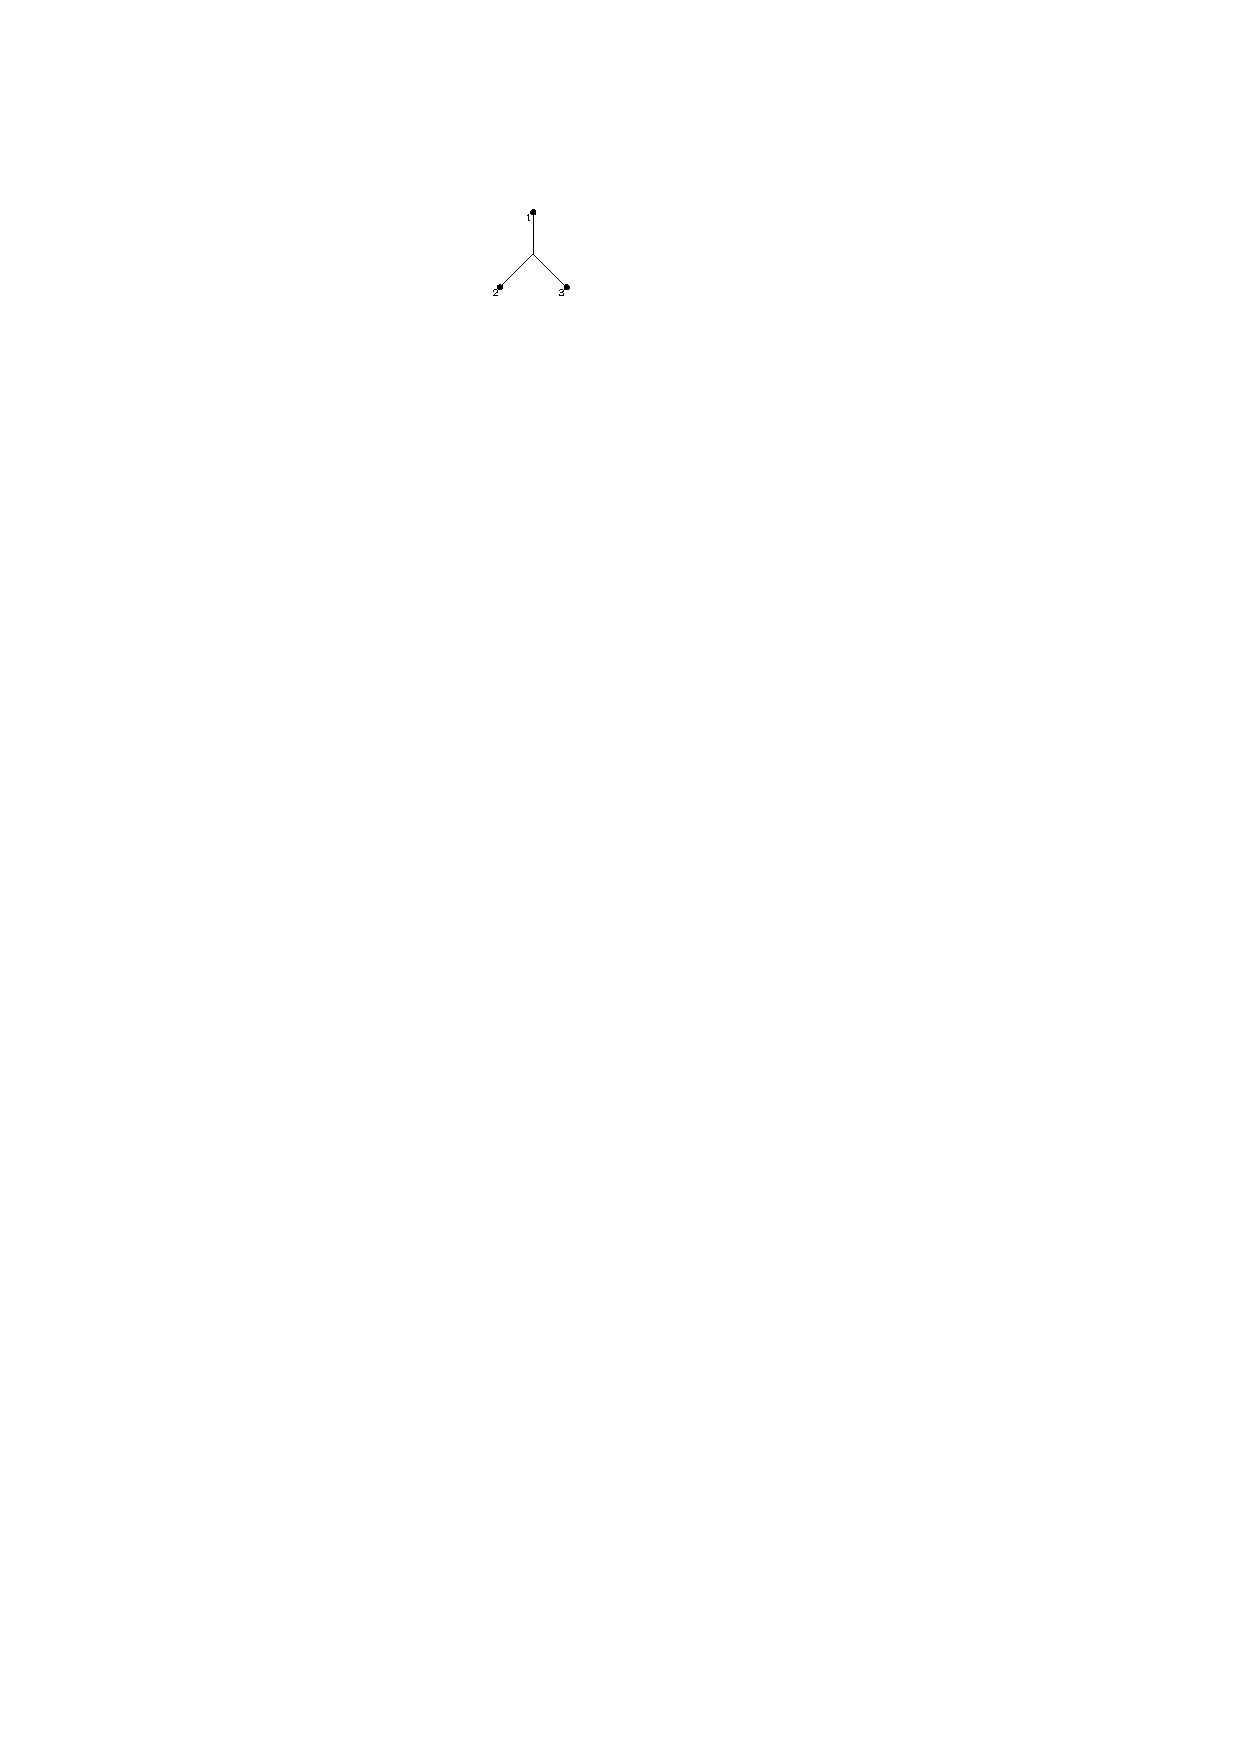
\includegraphics[scale=1.5]{fig/he1}
\hspace{2cm}
{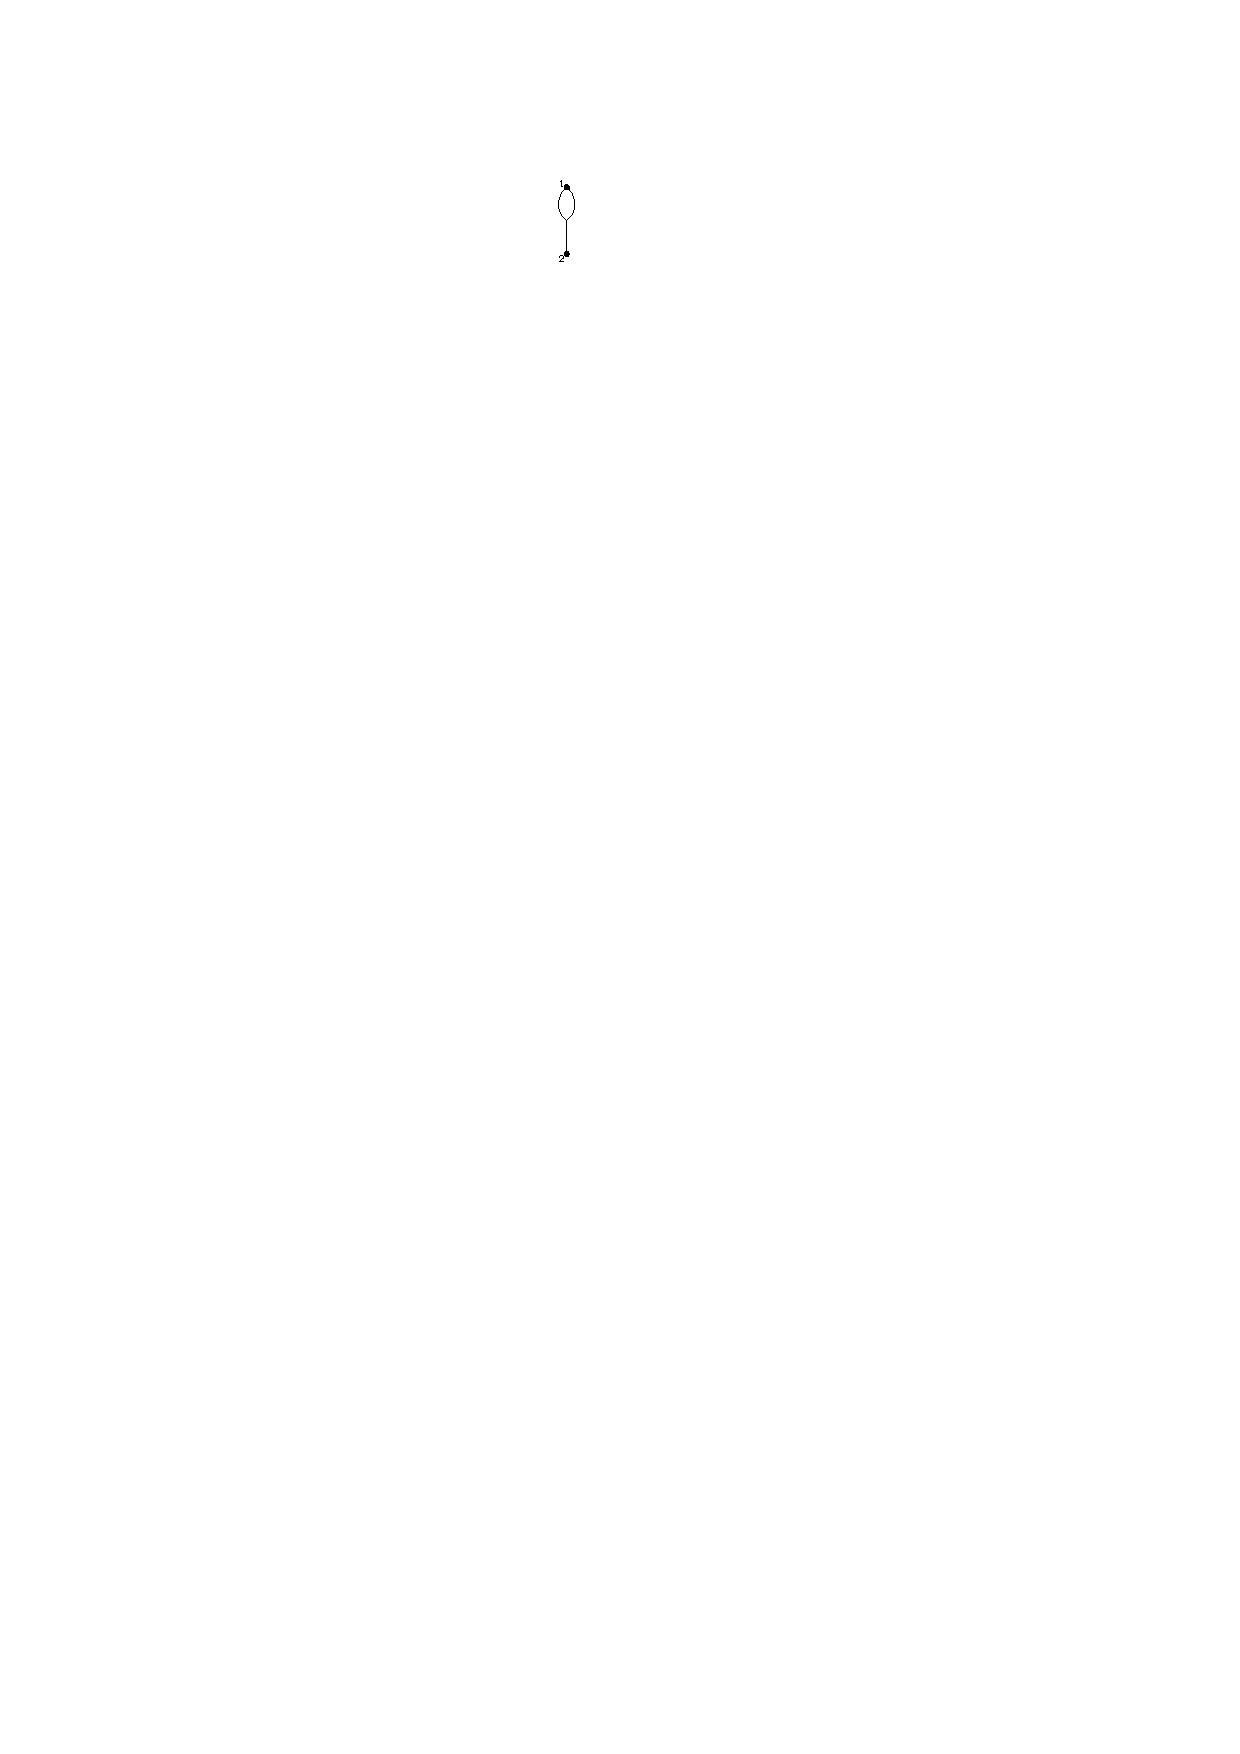
\includegraphics[scale=1.5]{fig/he2}}
\hspace{2cm}
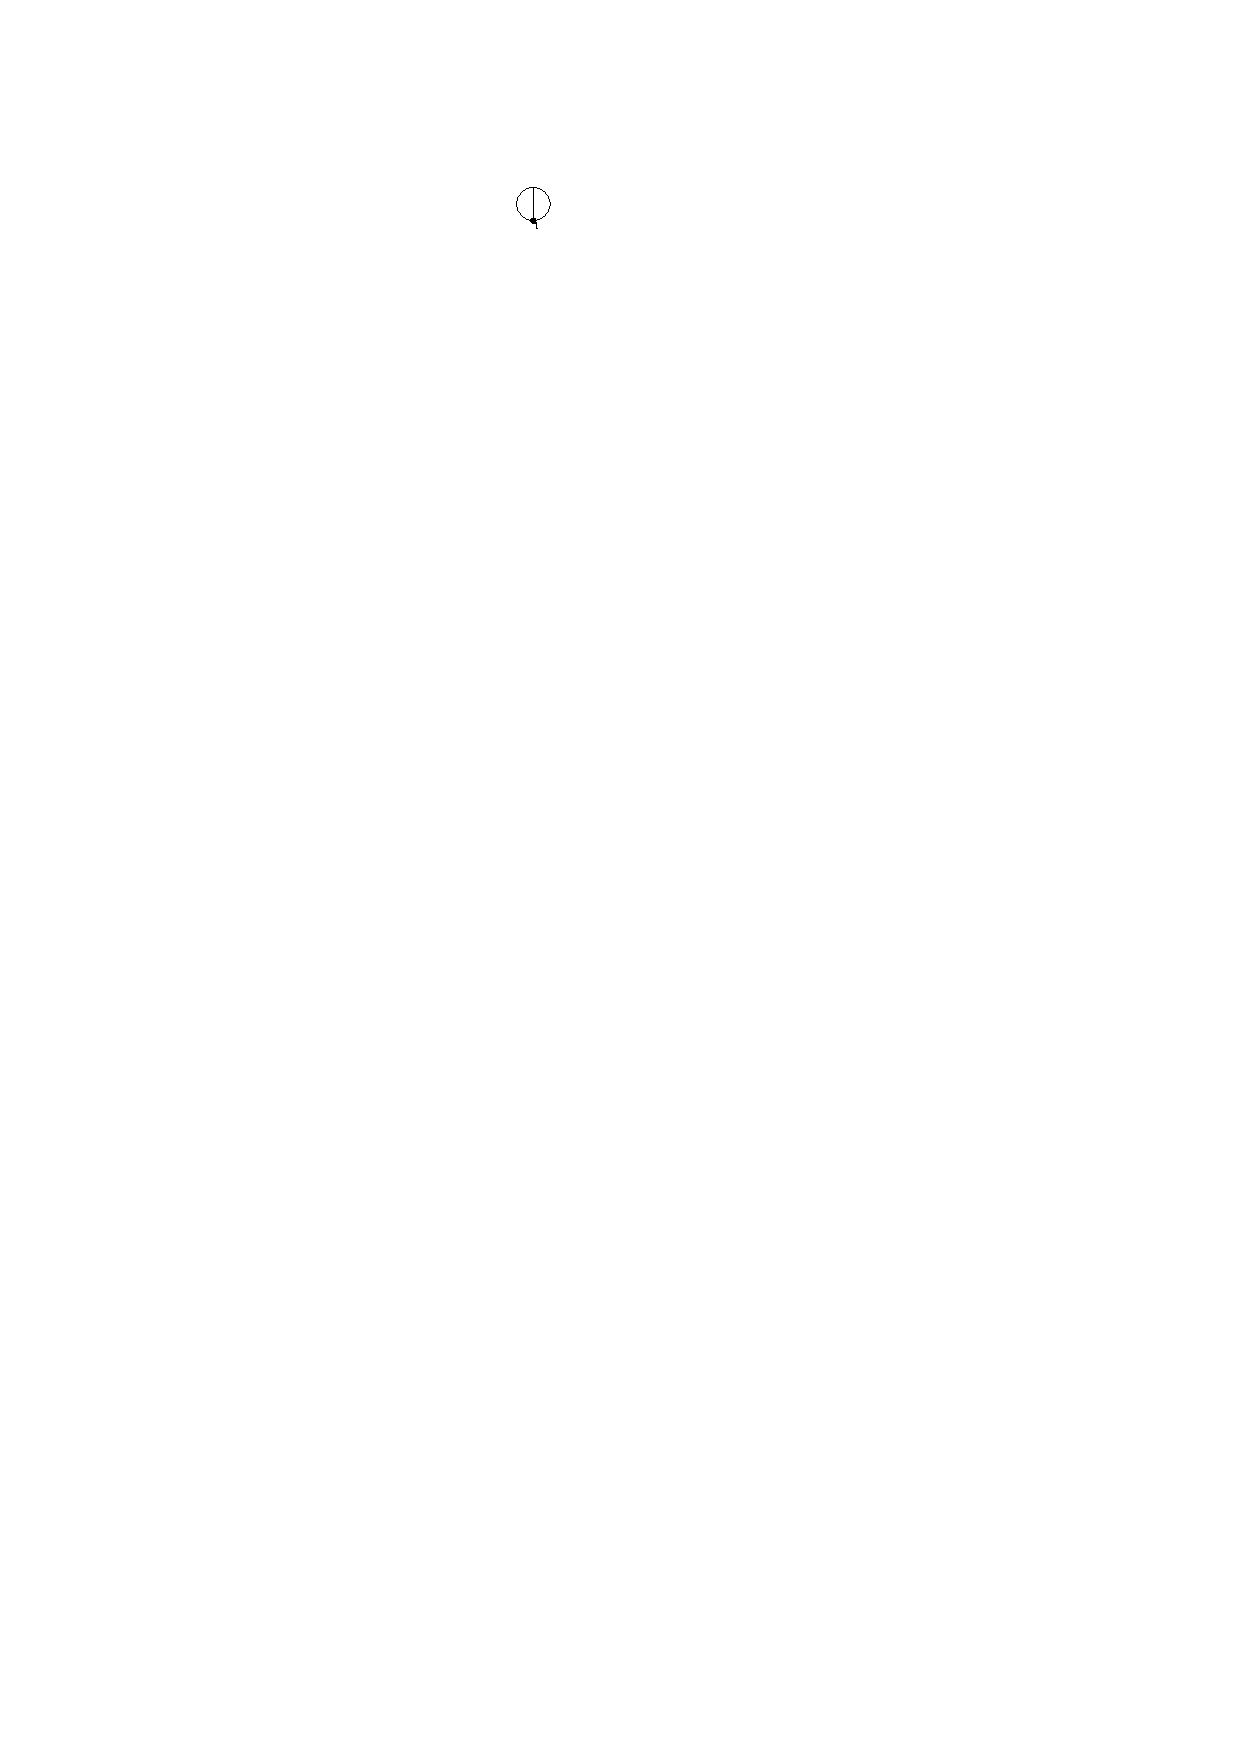
\includegraphics[scale=1.5]{fig/he3}
\caption{Three edges of cardinality 3.}
\label{e3}

\end{center}
\end{figure}
\begin{figure}[htbp]
\begin{center}
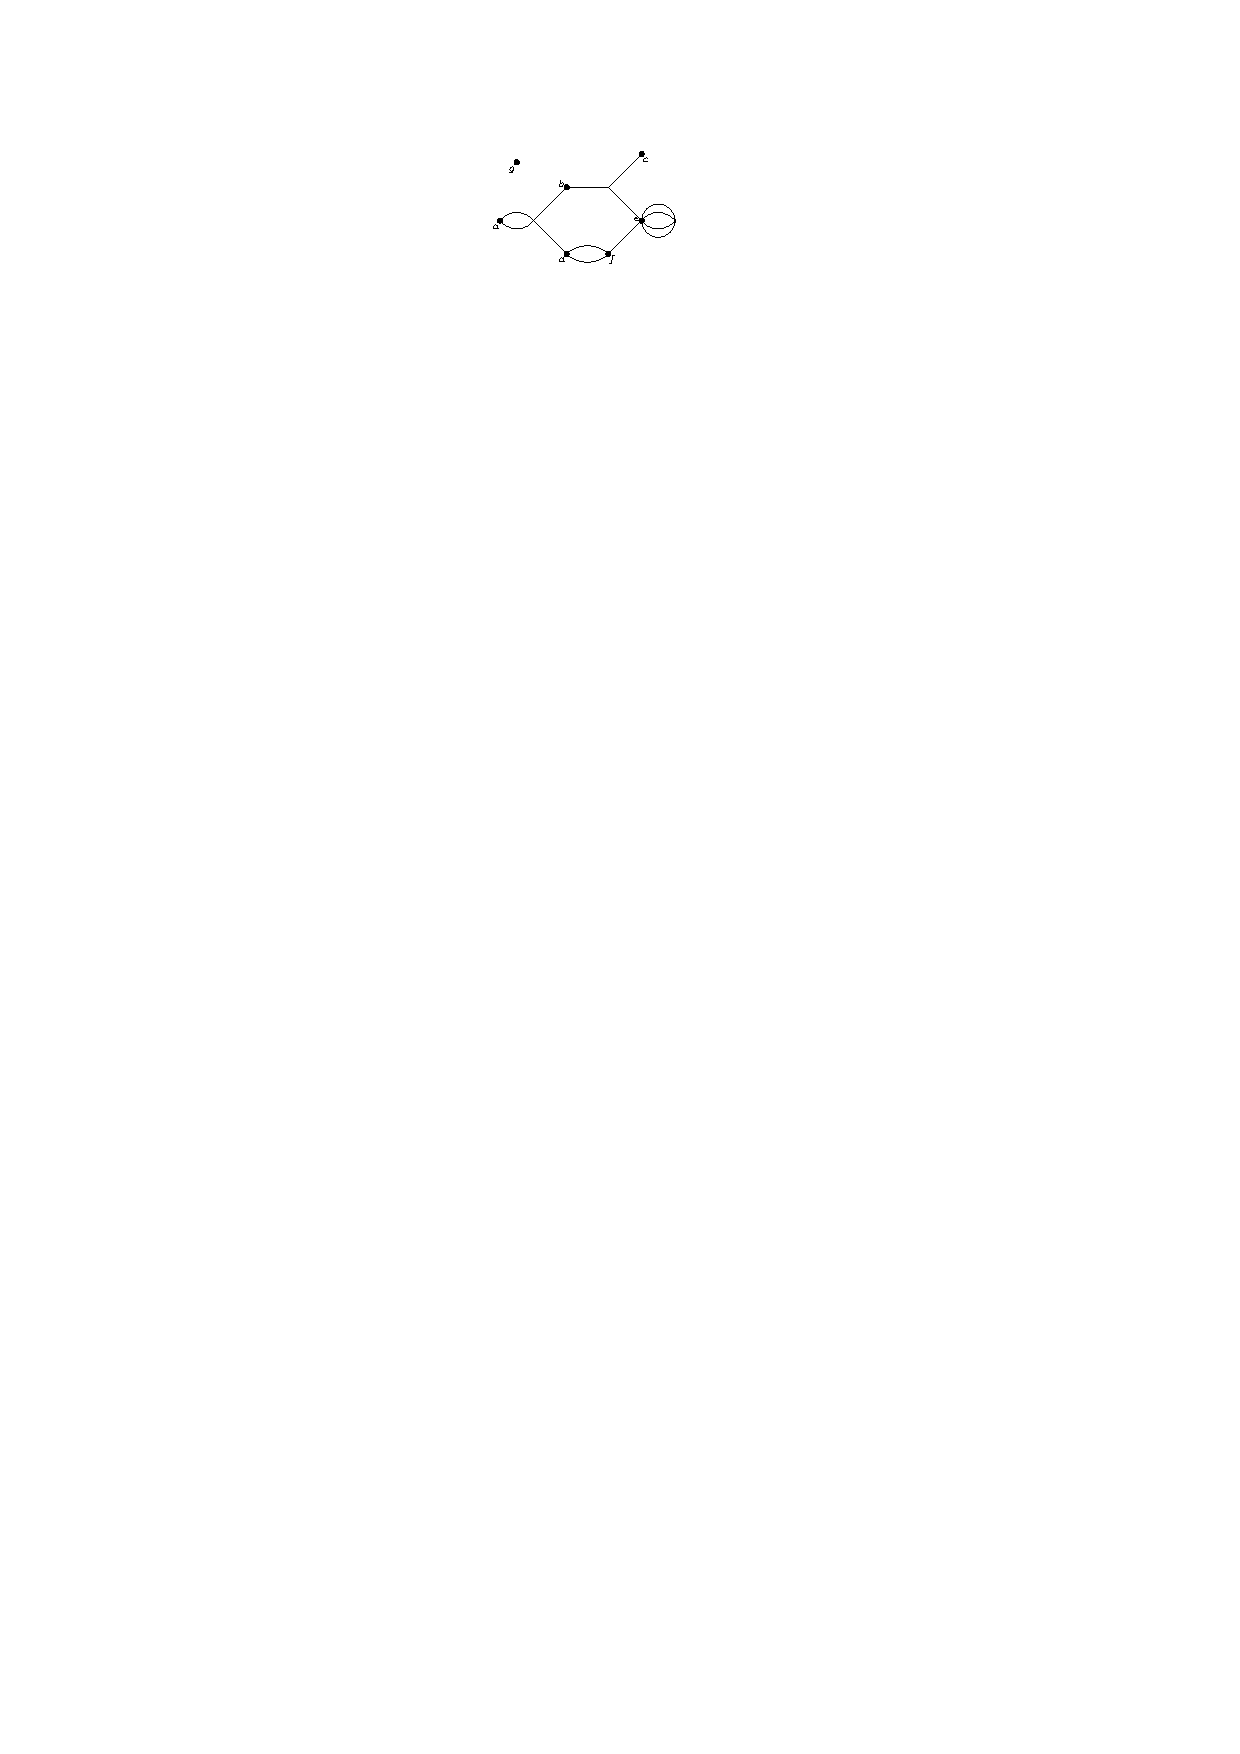
\includegraphics[scale=1.5]{fig/mhg1}
\caption{A multi-hypergraph over $\{a,b,c,d,e,f,g\}$.}
\label{mhg}
\end{center}
\end{figure}


\begin{example}
We represented the three edges $\{(1,1),(2,1),(3,1)\}$, $\{(1,2),(2,1)\}$ 
and $\{(1,3)\}$ in Figure \ref{e3} and the multi-hypergraph 
\begin{equation}
	\{(\{(a,2),(b,1),(d,1)\},1),(\{(b,1),(c,1),(e,1)\},1),(\{e,4\},1),(\{(e,1),(f,1)\},1),(\{(d,1),(f,1)\},2)\}
\end{equation}
over $\{a,b,c,d,e,f,g\}$ in Figure \ref{mhg}.
\end{example}

The set species $\MHG$ is isomorphic to the sub-species of $\text{Pol}$ 
of polynomials with constant term equal to 0. The isomorphism is defined 
as follows: for $V$ a finite set:
\begin{itemize}
\item the empty graph $\emptyset_V\in \MHG[V]$ is sent on the null polynomial $0_V$,
\item an edge $e$ is sent on the monomial $\prod_{v\in e} v^{e(v)}$,
\item an element $h\in \MHG[V]$ is sent on the polynomial $\bigoplus_{e\in h} e$.
\end{itemize}

We will often identify $\MHG$ with this sub-species. This identification 
will be very useful in the following to do computations since it is easier 
to formally write operations on polynomials than on graphs. With this 
identification, hypergraphs can be seen as polynomials where each variable 
appears at most once in each monomial and multigraphs as homogeneous polynomials of degree 2.

\begin{example}
With this identification, the multi-hypergraph in Example \ref{mhg} will be 
written as $a^2bd\oplus bce\oplus e^4\oplus ef\oplus df\oplus df$.
\end{example}


%%%%%%%%%%%%%%%%%%%%%%%%%%%%%%%%%%%%%%%%%%%%%%%%%%%%%%%%%%%%%%%%%%%%%%%%%%%%%%%%%%%
%%%%%%%%%%%%%%%%%%%%%%%%%%%%%%%%%%Constructions%%%%%%%%%%%%%%%%%%%%%%%%%%%%%%%%%%%%%%
%%%%%%%%%%%%%%%%%%%%%%%%%%%%%%%%%%%%%%%%%%%%%%%%%%%%%%%%%%%%%%%%%%%%%%%%%%%%%%%%%%%

\section{Species and operad construction}\label{sec:constructions}
To study the operads we are interested in, we will need to provide new ways 
of constructing species and operads from already existing ones. This is done in this section.

\begin{definition}
Let $A$ be a set and $S$ be a (resp set) species. A \textit{$A$-augmentation} 
of $S$ is a (resp set) species $A\text{-}S$ such that $A\text{-}S[V] \cong S[V\times A]$ for every finite set $V$.
\end{definition}


\begin{example}
Let $A$ be a set. Instead of considering an $A$-augmented multi-hypergraph on 
$V$ as a multi-hypergraph on $V\times A$, we see them as multi-hypergraphs on 
$V$ where the ends of the edges are labelled with elements of $A$. This is 
illustrated in Figure \ref{augm}. In particular, the set species of oriented 
graphs $G_{or}$ is the set sub-species of $\{(\_\text{(empty space)},>\}-G$ 
of graphs where each edge has exactly one non labelled end (i.e labeled by a empty space) and one end $>$.

Instead of seeing the variables of a polynomial in $A\text{-Pol}[V]$ as couples 
$(v,a)\in V\times A$, we see them as elements of $V$ indexed by elements of $A$: $v_a$.
\end{example}

\begin{equation}\label{augm}
	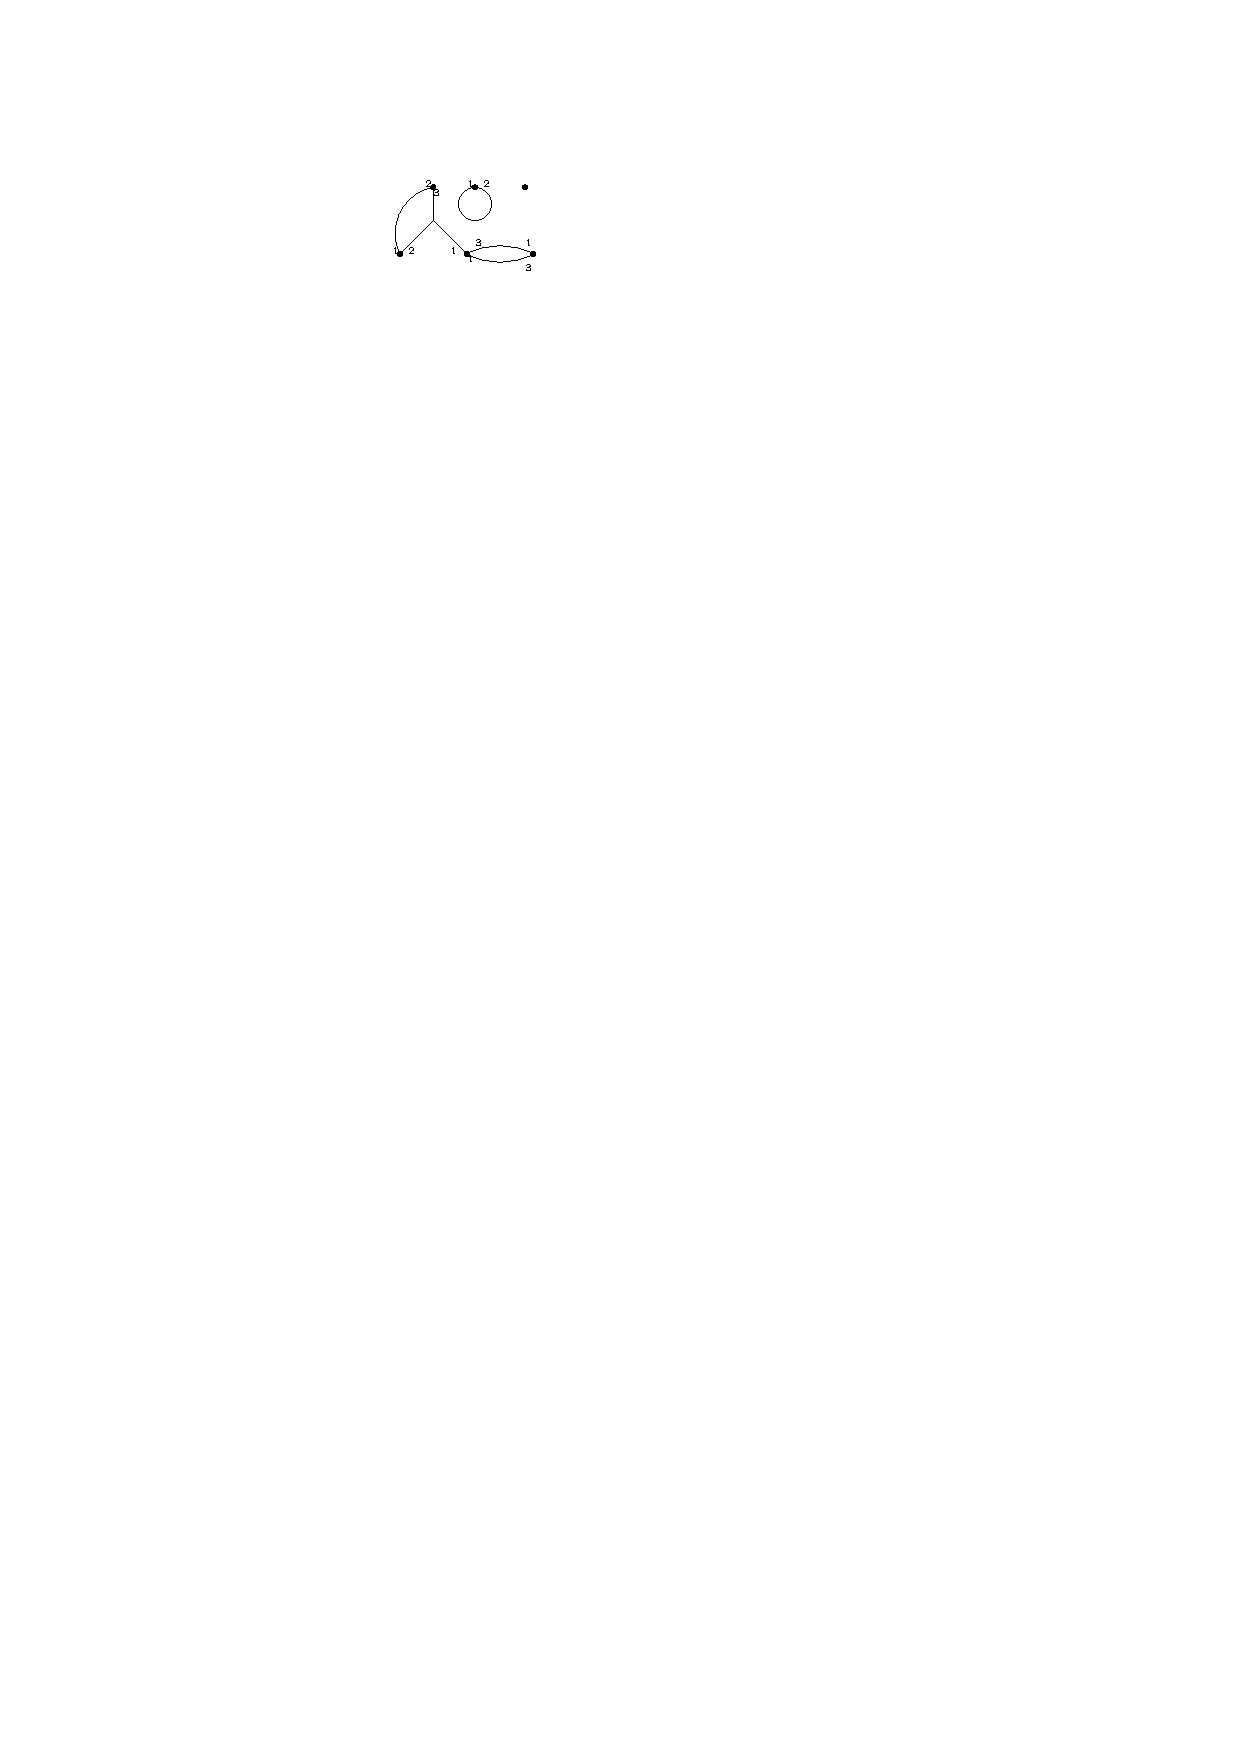
\includegraphics[scale=1.5]{fig/augm}
\end{equation}

\begin{proposition}
\label{semiprod}
	Let $S$ be a (resp set) species and $\op$ a set operad. Let $\varphi$ be a
 	collection of linear maps (resp maps) $\varphi_{V_1+\{\ast\},V_2}: 
 	(S[V_1+\{\ast\}]\otimes S[V_2]) \times \op[V_2] \rightarrow S[V_1+V_2]$ (resp
 	$S[V_1+\{\ast\}]\times S[V_2]$),
 	 where $V_1$ and $V_2$ are disjoint, such that: 
	\begin{itemize}
		\item for $x\in S[V_1+\{\ast_1\}]$, $(y,f)\in S\times\op[V_2+\{\ast_2\}]$ 
		and $(z,g)\in S\times\op[V_3]$:
		\begin{equation}
			\varphi_{V_1+\{\ast_1\},V_2+V_3}(x,\varphi_{V_2+\{\ast_2\},V_3}(y,z,g),f\circ_{\ast_2}g) = 
			\varphi_{V_1+V_2+\{\ast_2\},V_3}(\varphi_{V_1+\{\ast_1\},V_2+\{\ast_2\}}(x,y,f),z,g)
		\end{equation}
		\item for $x\in S[V_1+\{\ast_1,\ast_2\}]$, $(y,f)\in S\times\op[V_2]$ 
		and $(z,g)\in S\times\op[V_3]$:
		\begin{equation}
			\varphi_{V_1+V_2+\{\ast_2\},V_3}(\varphi_{V_1+\{\ast_1,\ast2\},V_2}(x,y,f),z,g) = 
			\varphi_{V_1+V_3+\{\ast_1\},V_2}(\varphi_{V_1+\{\ast_1,\ast2\},V_3}(x,z,g),y,f)
		\end{equation}
		\item there exists a map $e:X\rightarrow S$ such that for $(x,f)\in S\times\op[V]$ 
		and $(y,g)\in S\times\op[V+\{\ast\}]$ we have $\varphi_{\{\ast\},V}(e(\ast),x,f) = x$ 
		and $\varphi_{V+\{\ast\}, \{v\}}(x,e(v),e_{\op}(v)) = S[\tau_{\ast,v}](x)$ where 
		$e_{\op}$ is the unit of $\op$ and $\tau_{\ast,v}$ is the permutation which switches $\ast$ and $v$.
	\end{itemize}
	Then the partial composition $\circ^{\varphi}_{\ast}$ defined by:
	\begin{equation}\begin{split}
		\circ^{\varphi}_{\ast}: S\times\op[V_1+\{\ast\}]\otimes S\times\op[V_2] &\rightarrow S\times\op[V_1+V_2] \\
		(x,f)\otimes(y,g) &\mapsto (\varphi(x,y,g),f\circ_{\ast}g)
	\end{split}\end{equation}
	makes $S\times\op$ an (resp set) operad with unit $e$. We call this operad the 
	\textit{semidirect product of $S$ and $\op$ over $\varphi$} and we denote it by $S\ltimes_{\varphi}\op$.
\end{proposition}

\begin{proof}
This a rewritting a rewriting of the axioms of Definition \ref{op}.
\end{proof}

When clear in the context we will not mention $\varphi$ and just write 
semidirect product of $S$ and $\op$ and denote by $S\ltimes \op$. The 
goal of this construction is to give an operad structure to $S$ using 
the already known set operad structure on $\op$.

\begin{example}
{\color{red} Un peu plus compliqué qu'avant car il faut gérer les unités. peut être traiter se problème un mentionnant plus tôt que pour des opérades connexe (i.e $\op = X+\op_{2+}$) le produit partiel est trivial avec les éléments dans $\op[\{v\}]$}
Let $C$ be a finite set and denote by $C_{2+}$ the set species defined by 
$C_{2+}[V] = C$ if $|V|>1$ and $C_{2+}[V] = \emptyset$ else. The species 
$\mathcal{C}=X+C_{2+}$ has a set operad structure with partial composition 
defined by, for $x\in \mathcal{C}'[V_1]$ and $y\in C[V_2]$: $x\circ_{\ast} y = x$ 
if $V_1\not = \emptyset$ and $x\circ_{\ast} y = y$ else. Let $\mathcal{F}^C = X + 
\mathcal{F}_{2+}^C$ be the set species of maps with codomain $C$: 
$\mathcal{F}^C[V]=\{f:V\rightarrow C\}$ for $|V| > 1$. Then we have the 
semidirect product $\K\mathcal{F}^C\ltimes_{\varphi} \mathcal{C}$ given by, 
for $V_1\not = \emptyset$, $|V_2|>1$ and $f\in \mathcal{F}^C[V_1+\{\ast\}]$
 and $(g,x)\in \mathcal{F}^C\times \mathcal{C}[V_2]$: $\varphi(f,g,c) = 0$ 
 if $f(\ast) \not = c$ and $\varphi(f,g,c)(v) = \left\{\begin{array}{rl}
f(v)  & \text{if $v\in V_1$}    \\ 
g(v)  & \text{if $v\in V_2$}\end{array}\right.$ else. When $V_1=\emptyset$ 
or $|V_2|=1$ the partial composition is implied by definition of the unit. 
We call this operad the \textit{$C$-coloration} operad. Alone, one can see 
an element of $(f,c)\mathcal{F}^C\ltimes C[V]$ (with $|V|>1$) as a corolla 
on $V$ with its root colored by $c$ and its leaves $v\in V$ colored by $f(v)$. 
The partial composition consists then in grafting two corollas if the root and 
the leaf on which it must be grafted share the same colors. However this operad is 
more frequently in a Hadamard product with an other operad as a way to color it. 
\end{example}

% \begin{definition}
% Let $S$ be a (resp set) species. We call \textit{completion} of $S$ the (rest set) species $\overline{S}$ defined by $\overline{S}[V] = \bigoplus_{W\subseteq V}S[W]$ (resp union). If $\op$ is a (resp set) operad then $\overline{\op}$ also has an operad structure given by the following partial composition: for $x\in\overline{\op}'[V_1]$ and $y\in\overline{\op}[V_2]$ we have $x\circ_{\ast} y = \left\{\begin{array}{cl}
% x\circ_{\ast} y  & \text{if $x\in \op[W]$ and $\ast\in W$}    \\ 
% x & \text{else.}\end{array}\right.$
% \end{definition}

% Completed species are not usual in species theory or operad theory. The polynomial species $\text{Pol}$ given in Example \ref{notpol} is an example of a completed species.

\begin{definition}
Let $A$ be a set and $\op$ be an (resp set) operad with unit $e$. 
The set species of \textit{functions from $A$ to $\op$} is defined by 
$\mathcal{F}_A^{\op}[V] = \{f:A\rightarrow \op[V]\}$. This set species has 
a set operad structure with the elements $f:A \rightarrow \{e(v)\}$ in 
$\mathcal{F}_A^{\op}[\{v\}]$ as units and partial composition defined by 
$f_1\circ_{\ast} f_2(a) = f_1(a)\circ_{\ast} f_2(a)$.
\end{definition}

Remark that if $A$ is a singleton then $\mathcal{F}_A^{\op} \cong \op$.

Let $A,B,C,D$ four sets such that $A$ and $B$ are disjoint and $f:A\rightarrow C$ 
and $g:B\rightarrow D$ two maps. We denote by $f\uplus g$ the map from $A\sqcup B$ 
to $C\cup D$ defined by $f\uplus g(a) = f(a)$ for $a\in A$ and $f\uplus g(b) = g(b)$ 
for $b\in B$. 

\begin{proposition}
	Let $A$ and $B$ be two disjoint sets and $\op_1$ and $\op_2$ be two operads. 
	Then the set species $\mathcal{F}_A^{\op_1}\uplus\mathcal{F}_B^{\op_2}$ defined by 
	$\mathcal{F}_A^{\op_1}\uplus\mathcal{F}_B^{\op_2}[V] = \{f\uplus g\,|\, f\in\mathcal{F}_A^{\op_1}, g\in\mathcal{F}_B^{\op_2}\}$ 
	is a sub-operad of $\mathcal{F}_{A\sqcup B}^{\op_1+\op_2}$.
\end{proposition}

\begin{proof}
Since $A$ and $B$ are disjoint the partial composition is well defined and 
stable on $\mathcal{F}_A^{\op_1}\uplus\mathcal{F}_B^{\op_2}$.
\end{proof}

%%%%%%%%%%%%%%%%%%%%%%%%%%%%%%%%%%%%%%%%%%%%%%%%%%%%%%%%%%%%%%%%%%%%%%%%%%%%%%%%%%%%%%%%%%%%
%%%%%%%%%%%%%%%%%%%%%%%%%%%%%%%%%Graph operads%%%%%%%%%%%%%%%%%%%%%%%%%%%%%%%%%%%%%%%%%%%%
%%%%%%%%%%%%%%%%%%%%%%%%%%%%%%%%%%%%%%%%%%%%%%%%%%%%%%%%%%%%%%%%%%%%%%%%%%%%%%%%%%%%%%%%%%%%

\section{Graph operads}\label{sec:graph_operads}
In this section we will use the construction of the previous section to define operad 
structures on $\K \MHG$ and its sub-species.

\subsection{Graph insertion operads}
% The graph operads which are of interest to us are the operads where the partial composition works by "graph insertion"

% \subsection{The augmented multi-hypergraph operad}
% We give here a general method to construct graph insertion operads. This methods consists in giving a family of big operads such that most graph insertion operads (but not all) are isomorphic to a sub-operad or a quotient from one of these. The idea to construct these operads is to label the ends of the edges with a fixed set of labels and considering graphs (or hypergaphs or multigraphs) along with a function which associate to each label the vertices where the ends with label should go.

% %We present here a very general operad on graphs and their variants which includes many operads found in the literature such as the \PLie operad or hypergraphs operads presented in \cite{BV}. We then focus on a specific sub-operad and show a link with $\PLie$.

% Let us first introduce some terminology on multi-hypergraphs with labelled ends.

% \begin{definition}
% Let $A$ be a set and $V$ a finite set. An \textit{$A$-augmented end over $V$} is an element $(v,a)$ in $V\times A$, we call $v$ the vertex of the end and $a$ the augmentation of the end. An \textit{$A$-augmented edge over $V$} is multiset of $A$-augmented end over $V$ and an \textit{$A$-augmented multi-hypergraph over $V$} is a multiset of $A$-augmented edges. Note $A\text{-}\MHG$ the set species of $A$-augmented multi-hypergraphs.
% \end{definition}

% %For $A$ a set denote by $E_A$ the species of $A$-augemented ends, i.e $E_A[V] = V\times A$ and $EE_A$ the species of $A$-augmented edges i.e $EE_A[V] = \m(E_A[V])$.
% The forgetful functor $U:A\text{-}\MHG \rightarrow \MHG$ is defined by sending any $A$-augmented end $(v,a)$ of a $A$-augmented edges of a $A$-augmented multi-hypergraph on the end $v$. Given an edge $e$ over $V$, an $A$-augmentation of this edge is an $A$-augmented edge $e'$ over $V$ such that $U_V(e') = e$. Given a multi-hypergraph $h$, an $A$-augmentation of this multi-hypergraph is then a $A$-augmented multi-hypergraph $g'$ over $V$ such that $U_V(h') = h$.

% \begin{example}
% ...
% \end{example}


% Let $A$ be a set and $V$ a finite set. For $a\in A$ and $V\in v$, we will denote by:
% \begin{itemize}
% \item $v_a = (a,v)$ for $v\in V$ and $a\in A$,
% \item $\prod_{(v,a)\in e} v_a^{e((v,a))}$ for an $A$-augmented edge $e$ over $V$,
% \item $\emptyset_V$ the empty $A$-augmented multi-hypergraph over $V$,
% \item $\bigoplus_{e_i\in h}h(e_i)e_i$ for an $A$-augmented multi-hypergraph $h$.
% \end{itemize}
% These notations, along with $\emptyset_V\mapsto 0_V$, define a morphism from $A\text{-}\MHG[V]$ to $\text{Pol}[A\times V]$ which naturally extends to a morphism from $\K A\text{-}\MHG[V]$ to $\K\text{Pol}[A\times V]$. More precisely $A\text{-}\MHG$ is isomorphic to the sub-species of $V\mapsto \text{Pol}[A\times V]$ of polynomials with variables indexed by $A$ and with constant term equal to 0. 

% Frow now on we will identify $A\text{-}\MHG$ with this sub-species. This identification will be very useful in the following to do calculations since its easier to formally write operations on polynomials than on graphs. 


% \begin{definition}
% {\color{red} ou proposition ?}

% Let $\op$ be an operad with unit $e$ and $A$ a set.

% Note $\overline{\op}$ the operad defined by $\overline{\op}[V] = \bigcup_{W\subseteq V} \op[W]$, the partial composition being the same as in $\op$ except that $x\circ_{\ast}y = x$ if $x\in\op[V]$ and $\ast\not\in V$.

% Define the species of functions from $A$ to $\op$ by $\mathcal{F}_A^{\op}[V] = \{f:A\rightarrow \overline{\op}[V]\}$. Then $\mathcal{F}_A^{\op}$ has a set operad structure with the elements $f(A) = \{e(v)\}$ in $\mathcal{F}_A^{\op}[\{v\}]$ as units and partial composition defined by $f_1\circ_{\ast} f_2(a) = f_1(a)\circ_{\ast} f_2(a)$
% \end{definition}

% \begin{proposition}
% Let $A$ and $B$ be two disjoint sets and $\op_1$ and $\op_2$ be two operads. Then the set species $\mathcal{F}_A^{\op_1}\uplus\mathcal{F}_B^{\op_2}$ defined by $\mathcal{F}_A^{\op_1}\uplus\mathcal{F}_B^{\op_2}[V] = \{f\uplus g\,|\, f\in\mathcal{F}_A^{\op_1}, g\in\mathcal{F}_B^{\op_2}\}$, where $f\uplus g: a\in A\sqcup B \mapsto \delta_{a\in A}f(a)+\delta_{a\in B}g(a)$, is a sub-operad of $\mathcal{F}_{A\sqcup B}^{\op_1+\op_2}$.
% \end{proposition}

% \begin{proof}
% Since $A$ and $B$ are disjoint the partial composition is well defined and stable on $\mathcal{F}_A^{\op_1}\uplus\mathcal{F}_B^{\op_2}$.
% \end{proof}
% We can now give the announced operad.
Recall from Example \ref{notpol} that we denote by $\oplus$ the addition of 
polynomials and $0_{V}$ the zero polynomials in order to not confuse them with 
the addition of vectors and the null vector. As announced at the end of the 
subsection \ref{graph}, we will identify the elements of $\MHG$ with polynomials 
with null constant term. We will also identify $A$-augmented elements with 
polynomials with variables indexed by $A$.

We will now consider that the addition and multiplication of polynomials are 
distributive on the addition of vectors.

\begin{theorem}
\label{propins}
	Let $A$ be a set. Define the collection of maps $\varphi=\{\varphi_{V_1+\{\ast\},V_2}:
	(\K A\text{-}\MHG[V_1+\{\ast\}]\otimes\K A\text{-}\MHG[V_2])\times \mathcal{F}_A^{\K \MHG})[V_2]
	\rightarrow \K A\text{-}\MHG[V_1+V_2]\}_{V_1\cap V_2=\emptyset}$ by
	\begin{equation}
		\varphi(h_1,h_2,f) = h_1|_{\{\ast_a\leftarrow f(a)_a\}}\oplus h_2,
	\end{equation}
	where for a sum of polynomials $\sum P$, $(\sum P)_a = \sum P_a$ is the same sum 
	of polynomials but with all the variables indexed by $a$.

	We can then do the semidirect product of $\K A\text{-}\MHG$ and $\mathcal{F}_A^{\K \MHG}$ over $\varphi$.
\end{theorem}

We call any operad isomorphic to a sub-operad of $A\text{-}\MHG\ltimes\mathcal{F}_A^{\MHG}$ 
a {\em graph insertion} operad. The idea is to give a general construction of 
operads on (multi-)(hyper)graphs where the partial composition of two elements 
$g_1\circ_{\ast}g_2$ works as follows:
\begin{enumerate}
	\item do the disjoint union of $g_1$ and $g_2$,
	\item remove the vertex $\ast$ from $g_1$,
	\item connect \underline{independently} each loose ends of $g_1$ to $g_2$ in a certain way.
\end{enumerate}
\noindent What we mean by independently is that the way of connecting one end does not depend on 
how we connect the other ends. Note that the ``certain way'' in which an end can be 
connected include duplication of edges and augmenting the number of vertices of edges. 
Examples are given after the proof of Proposition \ref{propins}.

\begin{proof}
The linearity of $\varphi$ is given by the fact that the addition and multiplication of
 polynomials are distributive on the addition of vectors. We must verify that $\varphi$ 
 now verify the three items of Proposition \ref{semiprod}. The first two items are direct computations over polynomials:
\begin{equation}\begin{split}
	\varphi_{V_1+\{\ast_1\},V_2+V_3}(h_1,\varphi_{V_2+\{\ast_2\},V_3}(h_2,h_3,g),f\circ_{\ast_2}g) 
	&= h_1|_{\{\ast_{1a}\leftarrow f\circ_{\ast_2} g(a)_a\}}\oplus h_2|_{\{\ast_{2a}\leftarrow g(a)_a\}}\oplus h_3 \\
	&= h_1|_{\{\ast_{1a}\leftarrow f(a)_a\circ_{\ast_2} g(a)_a\}}\oplus h_2|_{\{\ast_{2a}\leftarrow g(a)_a\}}\oplus h_3 \\
	&= h_1|_{\{\ast_{1a}\leftarrow f(a)_a\}}|_{\{\ast_{2a}\leftarrow g(a)_a\}}\oplus h_2|_{\{\ast_{2a}\leftarrow g(a)_a\}}\oplus h_3 \\
	&= (h_1|_{\{\ast_{1a}\leftarrow f(a)_a\}}\oplus h_2)|_{\{\ast_{2a}\leftarrow g(a)_a\}}\oplus h_3 \\
	&=\varphi_{V_1+V_2+\{\ast_2\},V_3}(\varphi_{V_1+\{\ast_1\},V_2+\{\ast_2\}}(h_1,h_2,f),h_3,g)
\end{split}\end{equation}
\begin{equation}\begin{split}
	\varphi_{V_1+V_2+\{\ast_2\},V_3}(\varphi_{V_1+\{\ast_1,\ast2\},V_2}(h_1,h_2,f),h_3,g) 
	&= (h_1|_{\{\ast_{1a}\leftarrow f(a)_a\}}\oplus h_2)|_{\{\ast_{2a}\leftarrow g(a)_a\}}\oplus h_3 \\
	&= h_1|_{\{\ast_{1a}\leftarrow f(a)_a\}}|_{\{\ast_{2a}\leftarrow g(a)_a\}}\oplus h_2\oplus h_3 \\
	&= h_1|_{\{\ast_{2a}\leftarrow g(a)_a\}}|_{\{\ast_{1a}\leftarrow f(a)_a\}}\oplus h_3\oplus h_2 \\
	&= (h_1|_{\{\ast_{2a}\leftarrow g(a)_a\}}\oplus h_3)|_{\{\ast_{1a}\leftarrow f(a)_a\}}\oplus h_2 \\
	&= \varphi_{V_1+V_3+\{\ast_1\},V_2}(\varphi_{V_1+\{\ast_1,\ast2\},V_3}(h_1,h_3,g),h_2,f).
\end{split}\end{equation}

For the last item, let $e: X\rightarrow \text{-}\MHG$ be defined by $e(v) = \emptyset_{\{v\}}$. 
Then we have, with $e_{\mathcal{F}}$ the unit of $\mathcal{F}_A^{\MHG}$:
\begin{equation}
	\varphi_{\{\ast\},V}(e(\ast),h,f) = \emptyset_{\{\ast\}}|_{\{\ast_a \leftarrow f(a)_a\}}\oplus h = h.
\end{equation}
Moreover, we have:
\begin{equation}\begin{split}
	\varphi_{V+\{\ast\}, \{v\}}(h,e(v),e_{\mathcal{F}}(v)) 
	&= h|_{\{\ast_a \leftarrow e_{\mathcal{F}}(v)(a)_a\}}\oplus\emptyset_{\{v\}} \\
	&= h|_{\{\ast_a \leftarrow v_a\}} = A\text{-}\MHG[\tau_{(\ast,v)}](h).
\end{split}\end{equation}

This concludes the proof.
\end{proof}

In all the following when considering a semidirect product of a sub-species 
of $\K A\text{-}\MHG$ and a sub-operad of $\mathcal{F}_A^{\MHG}$, it will 
always be over the map $\varphi$ defined in the Proposition \ref{propins}, 
hence we will omit the $\varphi$ index.

From now on we will denote by $\sum V$ the sum $\sum_{v\in V} v$ in order 
to slightly lighten the computations.

Recall from the end of Example \ref{exop} that we have natural embeddings of 
$E$ and $Id$ in $\text{Pol}$ and a natural embedding of $\K E$ in $\K\text{Pol}$. 
Since the images of these embeddings have null constant term, these embeddings are in $\MHG$.
\begin{example}
 $G^{\bullet}$ has a natural set operad structure given by 
$G^{\bullet} \cong G\times Id \cong \{0\}\text{-}G\ltimes\mathcal{F}_{\{0\}}^{Id}$.
 For $(g_1,v_1)$ and $(g_2,v_2)$ two pointed graphs the partial composition 
 $(g_1,v_1)\circ_{\ast} (g_2,v_2)$ is then equal to $(g_3,v_1|_{\ast\leftarrow v_2})$ 
 where $g_3$ is the graph obtained by connecting all the ends on $\ast$ to $v_2$. More formally:
\begin{equation}\begin{split}
(g_1,v_1)\circ_{\ast} (g_2,v_2) &= (g_1|_{\ast\leftarrow v_2}\oplus g_2, v_1|_{\ast\leftarrow v_2}) \\
&= (G[\tau_{\ast,v_2}](g_1)\oplus g_2,v_1|_{\ast\leftarrow v_2}).
\end{split}\end{equation}
\begin{figure}[htbp]
\begin{center}
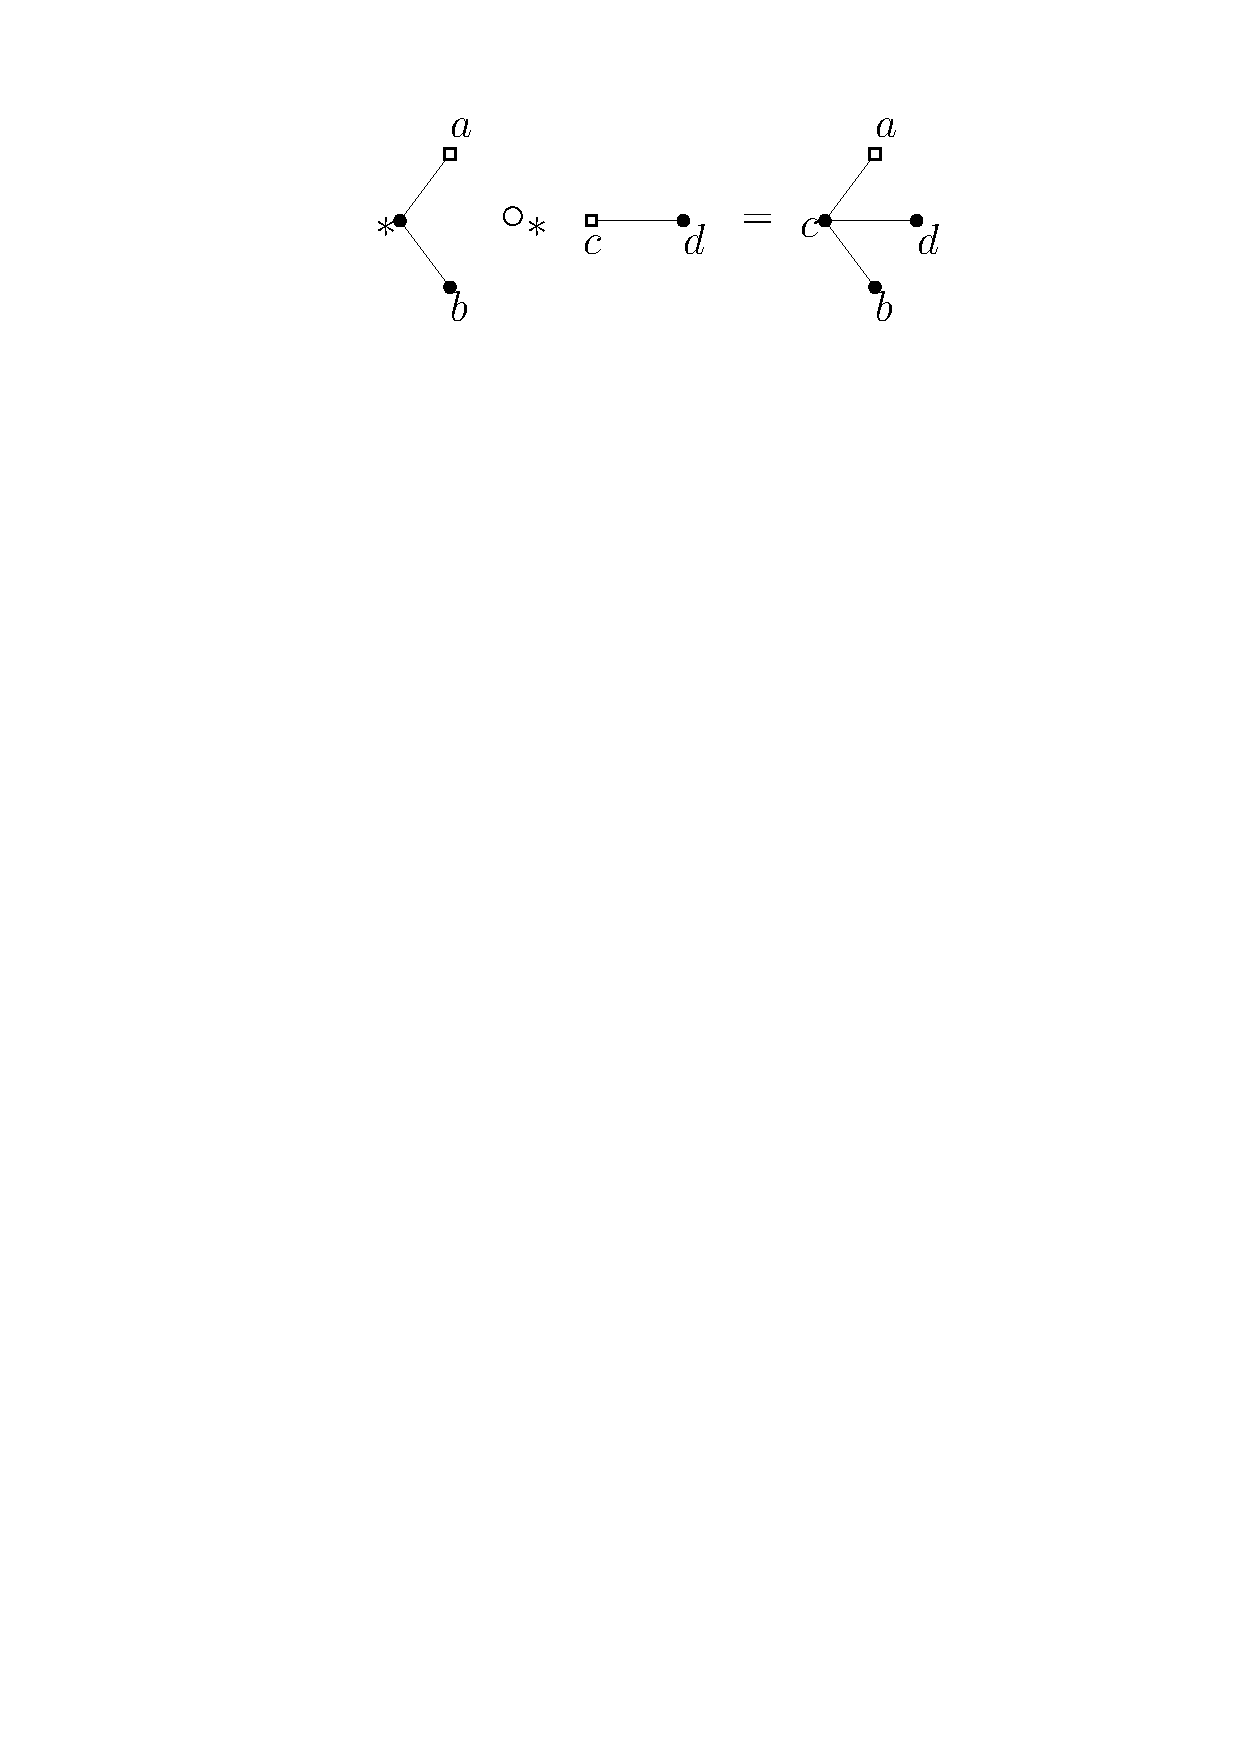
\includegraphics[scale=0.5]{fig/gcomp1}
\end{center}
\end{figure}

Remark that the set operad NAP~\cite{Liv06} is a set sub-operad of the operad above 
and hence is a graph insertion set operad.
\end{example}


\begin{example}
$G$ has a natural set operad structure given by 
$G\cong G\times E\cong \{0\}\text{-}G\ltimes\mathcal{F}_{\{0\}}^{E}$. 
For $g_1$ and $g_2$ two graphs the partial composition $g_1\circ g_2$ 
is then the graph obtained by adding an edge between each neighbour of 
$\ast$ and each vertex of $g_2$. More formally, for $g_1\in G'[V_1]$ and $g_2\in G[V_2]$:
\begin{equation}\begin{split}
	g_1\circ_{\ast} g_2 &= g_1|_{\ast \leftarrow \oplus_{v\in V_2} v}\oplus g_2\\
	&= g_1\cap V_1^2\oplus\bigoplus_{v\in n(\ast)}v(\bigoplus_{v'\in V_2} v')\oplus g_2 \\
	&= g_1\cap V_1^2\oplus\bigoplus_{v\in n(\ast)}\bigoplus_{v'\in V_2}vv'\oplus g_2,
\end{split}\end{equation}
where $n(\ast)$ is the set of neighbours of $\ast$. Note that we also 
consider $g_1$ as a set of edges here in order to write $g_1\cap V_1^2$ 
for the set of edges of $g_1$ not containing $\ast$.
\begin{figure}[htbp]
\begin{center}
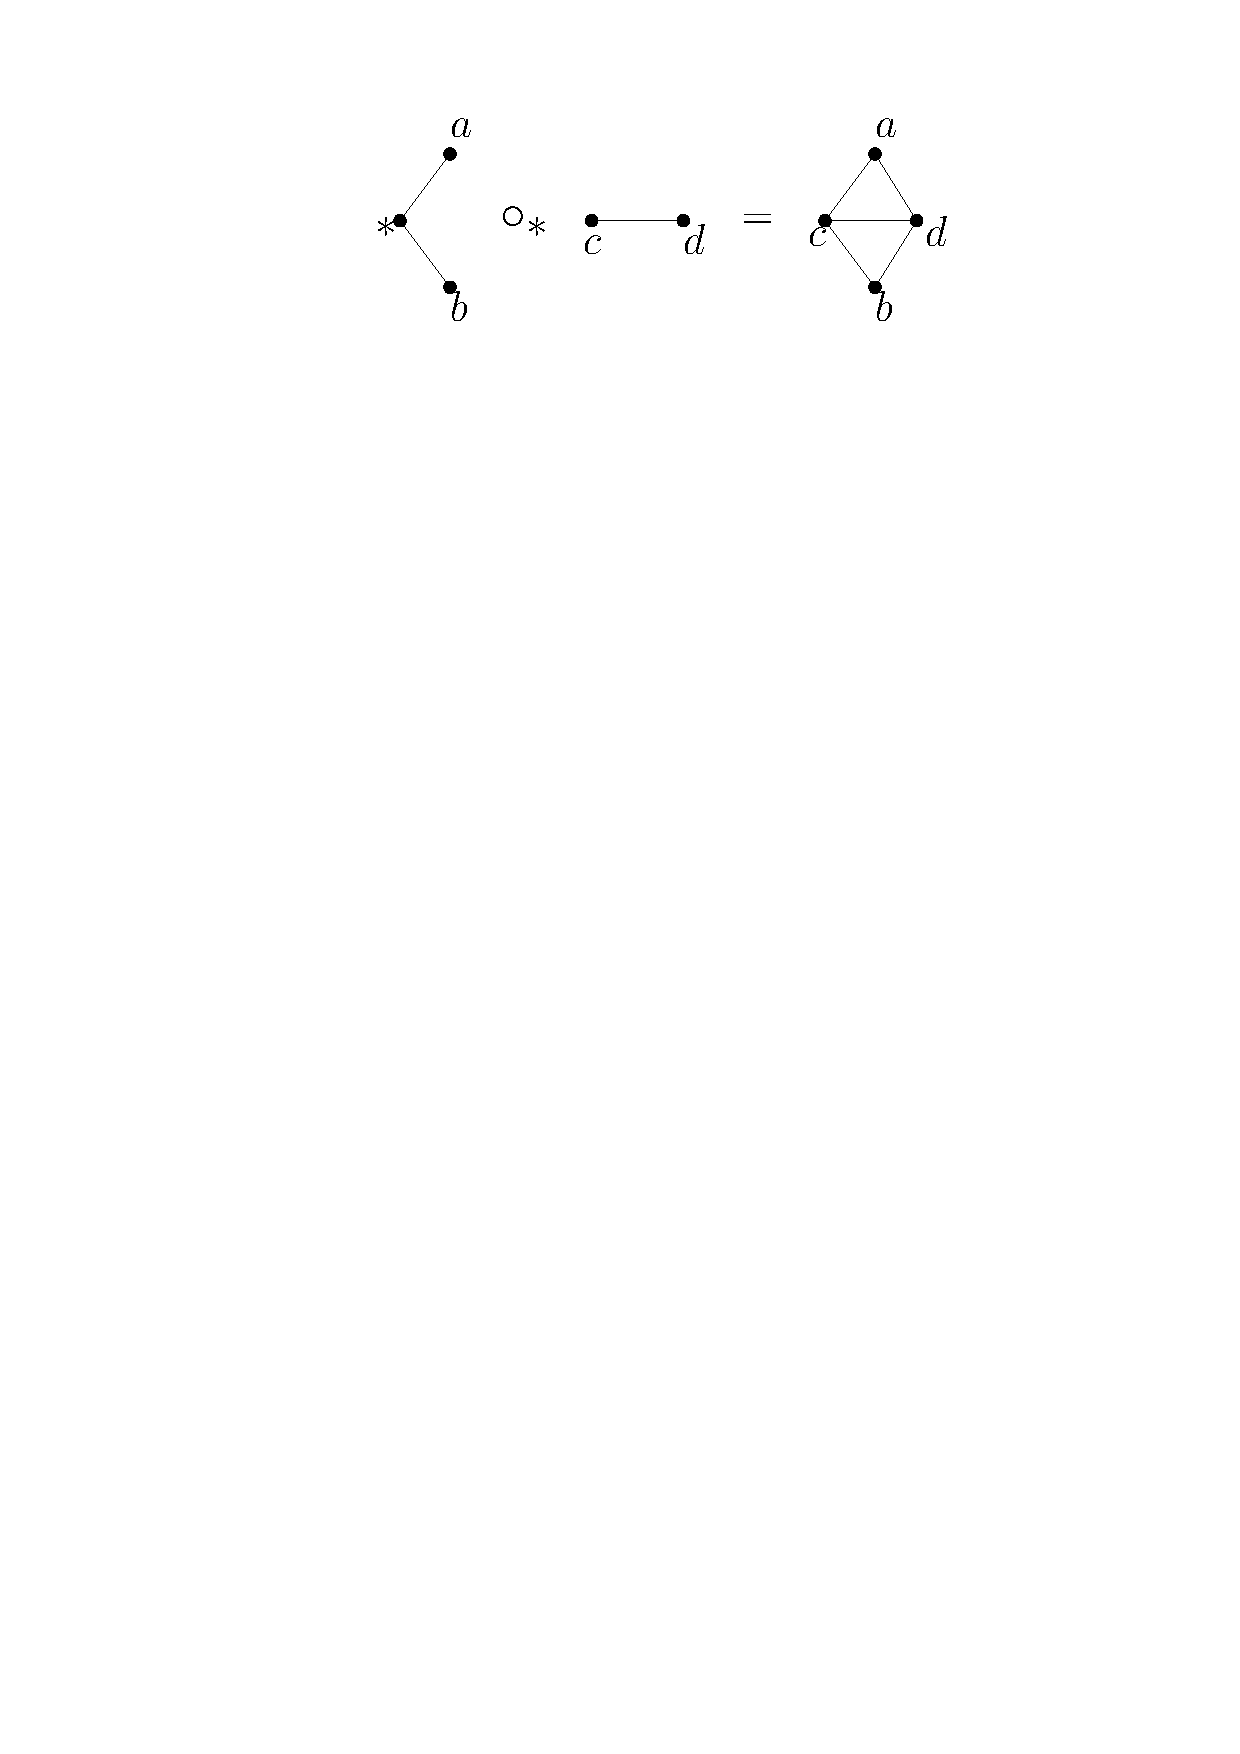
\includegraphics[scale=0.5]{fig/gcomp2}
\end{center}
\end{figure}
\end{example}

Let us now define two operads of interest with the help of Proposition~\ref{propins}

Let $V_1$ and $V_2$ be two disjoint sets.
For any multigraphs $g_1 \in \MG'[V_1]$ and $g_2 \in \MG[V_2]$, define
a partial composition of $g_1$ and $g_2$ as the sum of all the multigraphs
of $\MG[V_1 \setminus \sqcup V_2]$ obtained by the following process:
\begin{enumerate}
    \item Do the disjoint union of $g_1$ and $g_2$;
    \item Remove the vertex $\ast$. We then have some edges with one (or
    two if $\ast$ has loops) loose end(s);
    \item Connect each loose end to any vertex in $V_2$.
\end{enumerate}
For instance,
\begin{equation}\begin{split}
    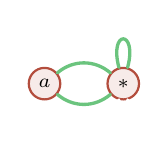
\begin{tikzpicture}[Centering,scale=1]
        \tikzset{every loop/.style={}}
        \node[NodeGraph](a)at(0,0){$a$};
        \node[NodeGraph](s)at(1,0){$\ast$};
        \draw[EdgeGraph](a)edge[bend left=40](s);
        \draw[EdgeGraph](a)edge[bend right=40](s);
        \draw[EdgeGraph](s)edge[loop above](s);
        \draw[EdgeGraph,draw=ColWhite](s)edge[loop below](s);
    \end{tikzpicture}
    \enspace \circ_\ast \enspace
    \begin{tikzpicture}[Centering,scale=1]
        \tikzset{every loop/.style={}}
        \node[NodeGraph](b)at(0,0){$b$};
        \node[NodeGraph](c)at(1,0){$c$};
        \draw[EdgeGraph](b)--(c);
        \draw[EdgeGraph](c)edge[loop above](c);
        \draw[EdgeGraph,draw=ColWhite](s)edge[loop below](s);
    \end{tikzpicture}
    & \enspace = \enspace
    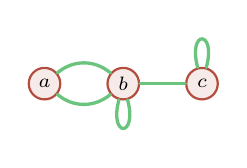
\begin{tikzpicture}[Centering,scale=1]
        \tikzset{every loop/.style={}}
        \node[NodeGraph](a)at(0,0){$a$};
        \node[NodeGraph](b)at(1,0){$b$};
        \node[NodeGraph](c)at(2,0){$c$}; 
        \draw[EdgeGraph](a)edge[bend left=40](b);
        \draw[EdgeGraph](a)edge[bend right=40](b);
        \draw[EdgeGraph](b)edge[loop below](b);
        \draw[EdgeGraph](b)--(c);
        \draw[EdgeGraph](c)edge[loop above](c);
    \end{tikzpicture}
    \enspace + \enspace
    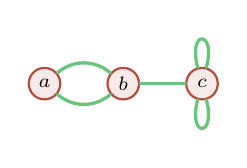
\begin{tikzpicture}[Centering,scale=1]
        \tikzset{every loop/.style={}}
        \node[NodeGraph](a)at(0,0){$a$};
        \node[NodeGraph](b)at(1,0){$b$};
        \node[NodeGraph](c)at(2,0){$c$};
        \draw[EdgeGraph](a)edge[bend left=40](b);
        \draw[EdgeGraph](a)edge[bend right=40](b);
        \draw[EdgeGraph](c)edge[loop below](c);
        \draw[EdgeGraph](b)--(c);
        \draw[EdgeGraph](c)edge[loop above](c);
    \end{tikzpicture}
    \enspace + \enspace
    2\,
    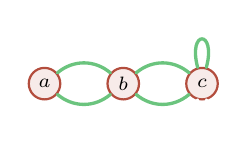
\begin{tikzpicture}[Centering,scale=1]
        \tikzset{every loop/.style={}}
        \node[NodeGraph](a)at(0,0){$a$};
        \node[NodeGraph](b)at(1,0){$b$};
        \node[NodeGraph](c)at(2,0){$c$};
        \draw[EdgeGraph](a)edge[bend left=40](b);
        \draw[EdgeGraph](a)edge[bend right=40](b);
        \draw[EdgeGraph](b)edge[bend left=40](c);
        \draw[EdgeGraph](b)edge[bend right=40](c);
        \draw[EdgeGraph](c)edge[loop above](c);
        \draw[EdgeGraph,draw=ColWhite](c)edge[loop below](c);
    \end{tikzpicture}
    \\
    & \quad + \enspace
    2\,
    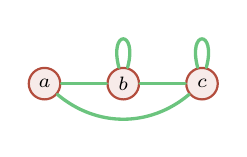
\begin{tikzpicture}[Centering,scale=1]
        \tikzset{every loop/.style={}}
        \node[NodeGraph](a)at(0,0){$a$};
        \node[NodeGraph](b)at(1,0){$b$};
        \node[NodeGraph](c)at(2,0){$c$};
        \draw[EdgeGraph](a)--(b);
        \draw[EdgeGraph](a)edge[bend right=40](c);
        \draw[EdgeGraph](b)edge[loop above](b);
        \draw[EdgeGraph](b)--(c);
        \draw[EdgeGraph](c)edge[loop above](c);
    \end{tikzpicture}
    \enspace + \enspace
    2\,
    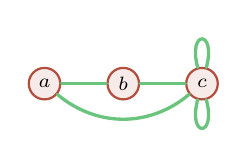
\begin{tikzpicture}[Centering,scale=1]
        \tikzset{every loop/.style={}}
        \node[NodeGraph](a)at(0,0){$a$};
        \node[NodeGraph](b)at(1,0){$b$};
        \node[NodeGraph](c)at(2,0){$c$};
        \draw[EdgeGraph](a)--(b);
        \draw[EdgeGraph](a)edge[bend right=40](c);
        \draw[EdgeGraph](c)edge[loop below](c);
        \draw[EdgeGraph](b)--(c);
        \draw[EdgeGraph](c)edge[loop above](c);
    \end{tikzpicture}
    \enspace + \enspace
    4\,
    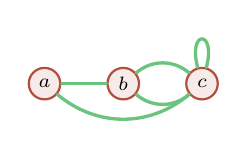
\begin{tikzpicture}[Centering,scale=1]
        \tikzset{every loop/.style={}}
        \node[NodeGraph](a)at(0,0){$a$};
        \node[NodeGraph](b)at(1,0){$b$};
        \node[NodeGraph](c)at(2,0){$c$};
        \draw[EdgeGraph](a)--(b);
        \draw[EdgeGraph](a)edge[bend right=40](c);
        \draw[EdgeGraph](b)edge[bend right=40](c);
        \draw[EdgeGraph](b)edge[bend left=40](c);
        \draw[EdgeGraph](c)edge[loop above](c);
    \end{tikzpicture}
    \\
    & \quad + \enspace
    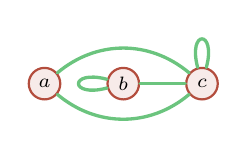
\begin{tikzpicture}[Centering,scale=1]
        \tikzset{every loop/.style={}}
        \node[NodeGraph](a)at(0,0){$a$};
        \node[NodeGraph](b)at(1,0){$b$};
        \node[NodeGraph](c)at(2,0){$c$};
        \draw[EdgeGraph](a)edge[bend right=40](c);
        \draw[EdgeGraph](a)edge[bend left=40](c);
        \draw[EdgeGraph](b)edge[loop left](b);
        \draw[EdgeGraph](b)--(c);
        \draw[EdgeGraph](c)edge[loop above](c);
    \end{tikzpicture}
    \enspace + \enspace
    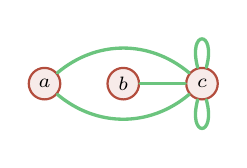
\begin{tikzpicture}[Centering,scale=1]
        \tikzset{every loop/.style={}}
        \node[NodeGraph](a)at(0,0){$a$};
        \node[NodeGraph](b)at(1,0){$b$};
        \node[NodeGraph](c)at(2,0){$c$};
        \draw[EdgeGraph](a)edge[bend right=40](c);
        \draw[EdgeGraph](a)edge[bend left=40](c);
        \draw[EdgeGraph](c)edge[loop below](c);
        \draw[EdgeGraph](b)--(c);
        \draw[EdgeGraph](c)edge[loop above](c);
    \end{tikzpicture}
    \enspace + \enspace
    2\,
    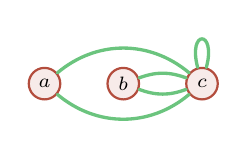
\begin{tikzpicture}[Centering,scale=1]
        \tikzset{every loop/.style={}}
        \node[NodeGraph](a)at(0,0){$a$};
        \node[NodeGraph](b)at(1,0){$b$};
        \node[NodeGraph](c)at(2,0){$c$};
        \draw[EdgeGraph](a)edge[bend right=40](c);
        \draw[EdgeGraph](a)edge[bend left=40](c);
        \draw[EdgeGraph](b)edge[bend left=20](c);
        \draw[EdgeGraph](b)edge[bend right=20](c);
        \draw[EdgeGraph](c)edge[loop above](c);
    \end{tikzpicture}.
\end{split}\end{equation}

\begin{theorem} \label{excano}
    The species $\K \MG$, endowed with the preceeding partial composition, is
    an operad.
\end{theorem}

\begin{proof}
This is the operad structure on $\K MG$ implied by the isomorphism of species 
$\K\MG\to \{0\}\text{-}MG\ltimes \mathcal{F}_{\{0\}}^{\K E}$.
\end{proof}


It is straightforward to observe that the
species $\K \G$ and $\K \MG_c$ are suboperads of $\K \MG$, that $\K \G_c$ a suboperad
of $\K \G$, and that $\K \T$ is a suboperad of $\K \G_c$. In particular, this structure on
$\K \G$ is known as the Kontsevich-Willwacher operad~\cite{MV19}. This partial composition
can be formally written as follows. For any $g_1 \in \MG[V_1]$ and $g_2 \in \MG[V_2]$ such
that $V_1$ and $V_2$ are two disjoint sets and $\ast \in V_1$,
\begin{equation}\begin{split}
	g_1\circ_{\ast} g_2 &= g_1|_{\ast \leftarrow \sum V_2}\oplus g_2\\
	&= g_1\cap V_1 \oplus\bigoplus_{v\in n(\ast)}v(\sum V_2)\oplus((\sum V_2)^2)^{\oplus g_1(\ast\ast)}\oplus g_2 \\
	&= \sum_{f:n(\ast)\to V_2}\sum_{l:[g_1(\ast\ast)]\to V_2V_2} g_1\cap V_1^2\oplus\bigoplus_{v\in n(\ast)}vf(v)\oplus\bigoplus_{i=1}^{g_1(\ast\ast)}l(i) \oplus g_2.
\end{split}\end{equation}
where $n(\ast)$ is the multiset of neighbours of $\ast$ in $g_1$ and $g_1(\ast\ast)$ is
the number of loops on $\ast$ in $g_1$. This partial composition reformulates in
a simpler way in on $\K\G$. For any $g_1 \in \G[V_1]$ and $g_2 \in \G[V_2]$ such
that $V_1$ and $V_2$ are two disjoint sets and $\ast \in V_1$, 
\begin{equation}\begin{split}
	g_1\circ_{\ast} g_2 &= g_1|_{\ast \leftarrow \sum V_2}\oplus g_2\\
	&= g_1\cap V_1 \oplus\bigoplus_{v\in n(\ast)}v(\sum V_2)\oplus g_2 \\
	&= \sum_{f:n(\ast)\rightarrow V_2} g_1\cap V_1^2\oplus\bigoplus_{v\in n(\ast)}vf(v)\oplus g_2.
\end{split}\end{equation}
where $n(\ast)$ is now the set of neighbour of $\ast$ in $g_1$. For instance,
\begin{equation}
    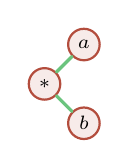
\begin{tikzpicture}[Centering,scale=.5]
        \node[NodeGraph](a)at(1,1){$a$};
        \node[NodeGraph](s)at(0,0){$\ast$};
        \node[NodeGraph](b)at(1,-1){$b$};
        \draw[EdgeGraph](a)--(s);
        \draw[EdgeGraph](s)--(b);
    \end{tikzpicture}
    \enspace \circ_\ast \enspace
    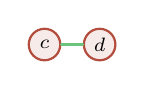
\begin{tikzpicture}[Centering,scale=.7]
        \node[NodeGraph](c)at(0,0){$c$};
        \node[NodeGraph](d)at(1,0){$d$};
        \draw[EdgeGraph](c)--(d);
    \end{tikzpicture}
    \enspace = \enspace
    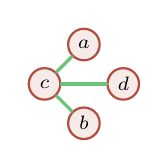
\begin{tikzpicture}[Centering,scale=.5]
        \node[NodeGraph](a)at(1,1){$a$};
        \node[NodeGraph](b)at(1,-1){$b$};
        \node[NodeGraph](c)at(0,0){$c$};
        \node[NodeGraph](d)at(2,0){$d$};
        \draw[EdgeGraph](c)--(a);
        \draw[EdgeGraph](c)--(d);
        \draw[EdgeGraph](c)--(b);
    \end{tikzpicture}
    \enspace + \enspace
    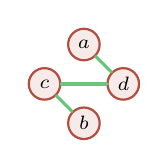
\begin{tikzpicture}[Centering,scale=.5]
        \node[NodeGraph](a)at(1,1){$a$};
        \node[NodeGraph](b)at(1,-1){$b$};
        \node[NodeGraph](c)at(0,0){$c$};
        \node[NodeGraph](d)at(2,0){$d$};
        \draw[EdgeGraph](c)--(d);
        \draw[EdgeGraph](d)--(a);
        \draw[EdgeGraph](c)--(b);
    \end{tikzpicture}
    \enspace + \enspace
    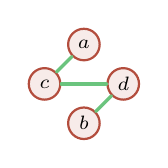
\begin{tikzpicture}[Centering,scale=.5]
        \node[NodeGraph](a)at(1,1){$a$};
        \node[NodeGraph](b)at(1,-1){$b$};
        \node[NodeGraph](c)at(0,0){$c$};
        \node[NodeGraph](d)at(2,0){$d$};
        \draw[EdgeGraph](c)--(d);
        \draw[EdgeGraph](c)--(a);
        \draw[EdgeGraph](d)--(b);
    \end{tikzpicture}
    \enspace + \enspace
    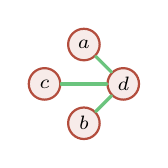
\begin{tikzpicture}[Centering,scale=.5]
        \node[NodeGraph](a)at(1,1){$a$};
        \node[NodeGraph](b)at(1,-1){$b$};
        \node[NodeGraph](c)at(0,0){$c$};
        \node[NodeGraph](d)at(2,0){$d$};
        \draw[EdgeGraph](c)--(d);
        \draw[EdgeGraph](d)--(a);
        \draw[EdgeGraph](d)--(b);
    \end{tikzpicture}.
\end{equation}
It is easy to observe that all graphs appearing $g_1 \circ_\ast g_2$ have $1$ as
coefficient. A formal formulation of the partial composition for multigraphs 
is also possible but the computations to handle the loops on $\ast$ would be too involved.

Let $V_1$ and $V_2$ be two disjoint sets such that $\ast \in V_1$. For any rooted oriented
multigraphs $(g_1, v_1) \in \MG_{or}^\bullet[V_1]$ and $(g_2, v_2) \in
\MG_{or}[V_2]^\bullet$, define a partial composition of $(g_1, v_1)$ and $(g_2, v_2)$ as
the sum of all the rooted multigraphs of $\MG_{or}^\bullet[V_1 \setminus \{\ast\} \sqcup
V_2]$ obtained by the following process:
\begin{enumerate}
    \item Do the disjoint union of $g_1$ and $g_2$;

    \item Remove the vertex $\ast$. We then have some edges with a loose end;

    \item Connect each non labelled loose end to $v_2$;

    \item Connect each labelled loose end to any vertex in $V_2$;

    \item The new root is $v_1$ if $v_1 \ne \ast$ and is $v_2$ otherwise.
\end{enumerate}
For instance, by depicting by squares the roots of the multigraphs,
\begin{equation}
 \label{canoor}
    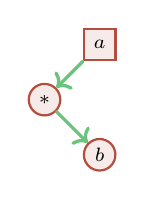
\begin{tikzpicture}[Centering,scale=.7]
        \node[NodeGraph](s)at(0,0){$\ast$};
        \node[RootGraph](a)at(1,1){$a$};
        \node[NodeGraph](b)at(1,-1){$b$};
        \draw[ArcGraph](a)--(s);
        \draw[ArcGraph](s)--(b);
    \end{tikzpicture}
    \enspace \circ_\ast \enspace
    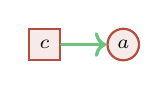
\begin{tikzpicture}[Centering,scale=1]
        \node[RootGraph](c)at(0,0){$c$};
        \node[NodeGraph](d)at(1,0){$a$};
        \draw[ArcGraph](c)--(d);
    \end{tikzpicture}
    \enspace = \enspace
    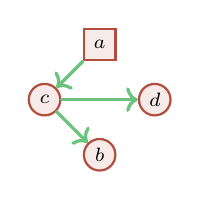
\begin{tikzpicture}[Centering,scale=.7]
        \node[RootGraph](a)at(1,1){$a$};
        \node[NodeGraph](b)at(1,-1){$b$};
        \node[NodeGraph](c)at(0,0){$c$};
        \node[NodeGraph](d)at(2,0){$d$};
        \draw[ArcGraph](a)--(c);
        \draw[ArcGraph](c)--(b);
        \draw[ArcGraph](c)--(d);
    \end{tikzpicture}
    \enspace + \enspace
    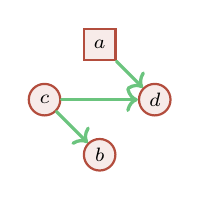
\begin{tikzpicture}[Centering,scale=.7]
        \node[RootGraph](a)at(1,1){$a$};
        \node[NodeGraph](b)at(1,-1){$b$};
        \node[NodeGraph](c)at(0,0){$c$};
        \node[NodeGraph](d)at(2,0){$d$};
        \draw[ArcGraph](a)--(d);
        \draw[ArcGraph](c)--(d);
        \draw[ArcGraph](c)--(b);
    \end{tikzpicture}
\end{equation}

\begin{theorem}
    The species $\K \MG_{orc}^\bullet$, endowed with the preceeding partial
    composition, is an operad.
\end{theorem}

\begin{proof}
This is the operad structure on $\K MG_{or}^{\bullet}$ implied by the monomorphism
$\K G_{or}^{\bullet} \hookrightarrow \{\_,>\} \text{-}G\ltimes\mathcal{F}_{\_}^{\K Id}\uplus\mathcal{F}_{>}^{\K E}$ 
defined by:
\begin{equation}\begin{split}
	\K \G_{or}^{\bullet}[V] &\hookrightarrow \{\_,>\}\text{-}\G\ltimes\mathcal{F}_{\_}^{\K Id}\uplus\mathcal{F}_{>}^{\K E}[V] \\
	(g,r) &\mapsto (g,f:\left\{\begin{array}{l}
	\_ \mapsto r \\
	> \mapsto \sum V\end{array}\right.).
\end{split}\end{equation}
\end{proof}

It is straightforward to observe that the subspecies of connected components $\K \MG^{\bullet}_{orc}$ 
and the species $\K \G^{\bullet}_{or}$ are suboperads of $\K \MG$ and that $\K \G^{\bullet}_{orc}$ is a 
suboperad of $\K \G^{\bullet}_{or}$. 
% For $\K \G_{or}^{\bullet}$, this partial composition 
% reformulates more formally as follows. For any $(g_1,v_1) \in \G_{or}^{\bullet}[V_1]$ 
% and $g_2 \in \G^{\bullet}[V_2]$ such that $V_1$ and $V_2$ are two disjoint sets and $\ast \in V_1$,
% \begin{equation}\begin{split}
% 	(g_1,v_1)\circ_{\ast} (g_2,v_2) 
% 	&= (g_1|_{\ast_{\_}\leftarrow v_{2\_},\, \ast_{>}\leftarrow (\sum V_2)_>}\oplus g_2, r_1|_{\ast\leftarrow r_2}) \\
% 	&= \left(g_1\cap V_1^2\oplus (\bigoplus_{v\in n_{\_}(\ast)}v_>v_{2\_})
% 	\oplus(\bigoplus_{v\in n_{>}(\ast)}v_{\_}(\sum V_2)_>)\oplus g_2, r_1|_{\ast\leftarrow r_2}\right) \\
% 	&= \sum_{f:n_{>}(\ast) \rightarrow V_2} \left(g_1\cap V_1^2\oplus (\bigoplus_{v\in n_{\_}(\ast)}v_>v_{2\_})
% 	\oplus(\bigoplus_{v\in n_{>}(\ast)}v_{\_}f(v)_>)\oplus g_2, r_1|_{\ast\leftarrow r_2}\right),
% \end{split}\end{equation}
% where for a label $a$, $n_{a}(\ast)$ is the set of neighbours $v$ of $\ast$ such that 
% label $a$ is on the $\ast$ end of the edge $v\ast$.

In a rooted tree, each edge has a parent end and a child end. Given a rooted tree $t$ with
root $r$, denote by $t_r$ the oriented tree where each parent end of $t$ is labelled and
each child end is non labelled. Then, the monomorphism $\T^{\bullet}\hookrightarrow
\G_{orc}^{\bullet}$ which sends each ordered pair $(t,r)$, where $t$ is a tree and $r$ is
its root, on $(t_r,r)$ induces an operad structure on the species of rooted trees which is
exactly the operad $\PLie$. Hence $\PLie$ is a graph insertion operad.

For the sake of completness, let us finish this section by mentioning 
that the notion of graph insertion operad introduced here is different 
than the one in \cite{Kreimer:2000ja}.

% The operad $\PLie$ is a graph insertion operad. More precisely, in a rooted tree each edge has a parent end and a child end. Given a tree $t$, denote by $t_{p,c}$ the $\{p,c\}$-augmented tree where each parent end of $t$ is labelled by $p$ and each child end is labelled by $c$. Then the following monomorphism:
% \begin{equation}\begin{split}
% \psi:\K T^{\bullet}[V] &\hookrightarrow \K \{p,c\}\text{-}T\times \mathcal{F}_{\{p\}}^{\K E}\uplus\mathcal{F}_{\{c\}}^{Id}[V] \\
% (t,r) &\mapsto (t_{p,c}, f:\left\{\begin{array}{l}
% p\mapsto \sum_{v\in V} v\\
% c\mapsto r\end{array}\right.),
% \end{split}\end{equation}
% gives $T^{\bullet}$ the $\PLie$ operad structure. More formally, for $(t_1,r_1)\in T^{\bullet}[V_1+\{\ast\}]$ and $(t_2,r_2)\in T^{\bullet}[V_2]$:
% \begin{equation}\begin{split}
% (t_1,r_1)\circ_{\ast} (t_2,r_2) &= (t_1\cap V_1^2\oplus p(\ast)r_2\oplus\bigoplus_{v\in c(\ast)}v(\sum_{v'\in V_2}v')\oplus t_2,r_1|_{\ast\leftarrow r_2}) \\
% &= \sum_{f:c(\ast)\rightarrow V_2} (t_1\cap V_1^2\oplus p(\ast)r_2\oplus\bigoplus_{v\in c(\ast)}vf(v)\oplus t_2,r_1|_{\ast\leftarrow r_2}),
% \end{split}\end{equation}
% where $p(\ast)$ is the parent of $\ast$ and $c(\ast)$ is the set of children of $\ast$. This is exactly the $\PLie$ structure.

% \begin{proposition}
% Let $A$ be a set. The species $\K A\text{-}\MHG\times\mathcal{F}_A^{\MHG}$ has an operad structure given by:
% \begin{itemize}
% \item the units $(\emptyset_{\{v\}},A\mapsto v)$,
% \item the partial composition $(h_1,f_1)\circ_{\ast} (h_2,f_2) = (h_1|_{\{\ast_a \leftarrow f_2(a)\}_{a\in A}}\oplus h_2, f_1\circ_{\ast}f_2)$.
% \end{itemize}
% Where the partial composition on functions was defined previously.
% \end{proposition}

% \begin{proof}
% It is clear that the partial composition is a species morphism. Let us show that it verifies the necessary axioms.

% Let $V_1$, $V_2$ and $V_3$ be three disjoint sets.
% \begin{itemize}
% \item Let be $(h_1,f_1)\in (A\text{-}\MHG\times \mathcal{F}_A)[V_1+\{\ast_1,\ast_2\}]$,  $(h_2,f_2)\in (A\text{-}\MHG\times \mathcal{F}_A)[V_2]$ and $(h_3,f_3)\in(A\text{-}\MHG\times \mathcal{F}_A)[V_3]$. Then:
% \begin{equation}\begin{split}
% ((h_1,f_1)&\circ_{\ast_1}(h_2,f_2))\circ_{\ast_2} (h_3,f_3) \\
% &= (h_1|_{\{\ast_{1a}\leftarrow f_2(a)\}_{a\in A}}\oplus h_2, f_1\circ_{\ast_1}f_2)\circ_{\ast_2}(h_3,f_3) \\
% &= (h_1|_{\{\ast_{1a}\leftarrow f_2(a)\}_{a\in A}}|_{\{\ast_{2a}\leftarrow f_3(a)\}_{a\in A}}\oplus h_2|_{\{\ast_{2a}\leftarrow f_3(a)\}_{a\in A}}\oplus h_3, (f_1\circ_{\ast_1}f_2)\circ_{\ast_2}f_3) \\
% &= (h_1|_{\{\ast_{2a}\leftarrow f_3(a)\}_{a\in A}}|_{\{\ast_{1a}\leftarrow f_2(a)\}_{a\in A}}\oplus h_3|_{\{\ast_{1a}\leftarrow f_2(a)\}_{a\in A}}\oplus h_2, (f_1\circ_{\ast_2}f_3)\circ_{\ast_1}f_2) \\
% &= (h_1|_{\{\ast_{2a}\leftarrow f_3(a)\}_{a\in A}}\oplus h_3, f_1\circ_{\ast_2}f_3)\circ_{\ast_1}(h_2,f_2) \\
% &= ((h_1,f_1)\circ_{\ast_2}(h_3,f_3))\circ_{\ast_1} (h_2,f_2),\end{split}\end{equation}
% \item Let be $(h_1,f_1)\in (A\text{-}\MHG\times \mathcal{F}_A)[V_1+\{\ast_1\}]$,  $(h_2,f_2)\in (A\text{-}\MHG\times \mathcal{F}_A)[V_2+\{\ast_2\}]$ and $(h_3,f_3)\in(A\text{-}\MHG\times \mathcal{F}_A)[V_3]$. Then:
% \begin{equation}\begin{split}
% ((h_1,f_1)&\circ_{\ast_1}(h_2,f_2))\circ_{\ast_2} (h_3,f_3) \\
% &= (h_1|_{\{\ast_{1a}\leftarrow f_2(a)\}_{a\in A}}\oplus h_2, f_1\circ_{\ast_1}f_2)\circ_{\ast_2}(h_3,f_3) \\
% &= (h_1|_{\{\ast_{1a}\leftarrow f_2(a)\}_{a\in A}}|_{\{\ast_{2a}\leftarrow f_3(a)\}_{a\in A}}\oplus h_2|_{\{\ast_{2a}\leftarrow f_3(a)\}_{a\in A}}\oplus h_3, (f_1\circ_{\ast_1}f_2)\circ_{\ast_2}f_3) \\
% &= (h_1|_{\{\ast_{1a}\leftarrow f_2\circ_{\ast_2} f_3(a)\}_{a\in A}}\oplus h_2|_{\{\ast_{2a}\leftarrow f_3(a)\}_{a\in A}}\oplus h_3, f_1\circ_{\ast_1}(f_2\circ_{\ast_2}f_3)) \\
% &= (h_1,f_1)\circ_{\ast_1}((h_2, f_2)\circ_{\ast_2}(h_3,f_3)),
% \end{split}\end{equation}
% \item Let $v\not\in V_1$ and $(h,f)\in (A\text{-}\MHG\times \mathcal{F}_A)[V_1]$ and $(h',f')\in (A\text{-}\MHG\times \mathcal{F}_A)[V_1+\{\ast\}]$. Then $(\emptyset_{\{\ast\}},A\mapsto\{\ast\})\circ_{\ast} (h,f) = (h,f)$ and $(h',f')\circ_{\ast}(\emptyset_{\{v\}}, A\mapsto \{v\}) = A\text{-}\MHG[\ast\mapsto v](h',f')$
% \end{itemize}
% \end{proof}



\subsection{Canonical graph operad}
We study here in more details the operad structure on $\K \G$ implied by the one 
on $\K \MG$ given in Theorem \ref{excano}. 
% We consider these operad structures as
%  canonical on $\K G_c$ and $\K G$, and from now on we mention them as the operad 
%  $\K G_c$ and the operad $\K G$. 
We will see that while $\K \G$ itself has an 
 evolved operadic structure, it has many interesting sub-operads.

Before explaining how $\K G$ is complicated, let us first introduce some notations.
Let $S$ be a species, $I$ be a set, $\{V_i\}_{i\in I}$ be a family of finite sets, and
$x_i\in S[V_i]$ for all $i\in I$. We call {\em subspecies of $S$ generated by $\{x_i\}_{i\in I}$}
the smallest subspecies of $S$ containing the family $\{x_i\}_{i\in I}$.
If $S$ is furthermore an operad, we call {\em suboperad of $S$ generated by $\{x_i\}_{i\in I}$}
the smallest suboperad of $S$ containing the family $\{x_i\}_{i\in I}$. We write that {\em $x$ is
generated by $\{x_i\}_{i\in I}$} if $x$ is in the suboperad generated by $\{x_i\}_{i\in I}$.

% \begin{example}
% We have that $\K G = E(G_c) = <\bigcup_{n>0}G_c[[n]] + \{\raisebox{-4pt}{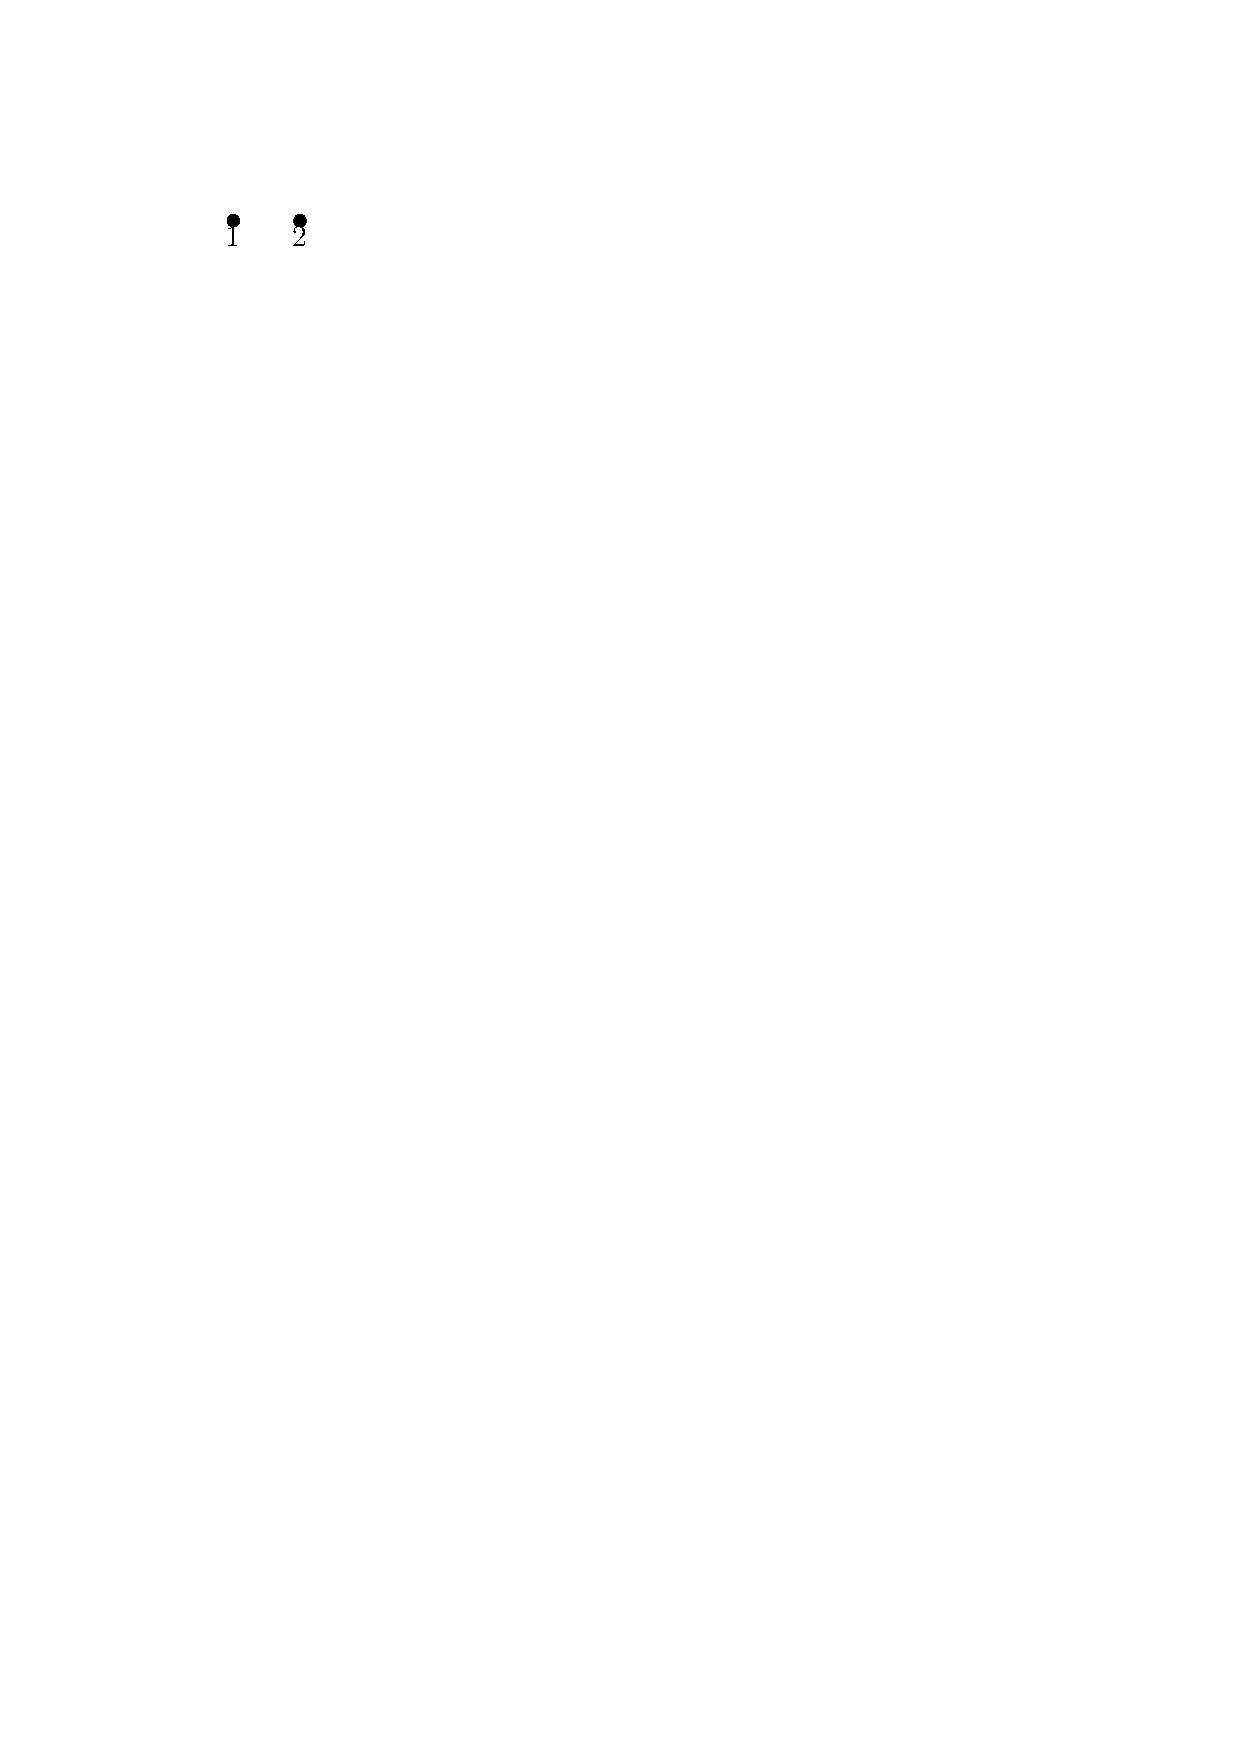
\includegraphics[scale=0.5]{fig/pts}}\}>^{Ope}$ since the disjoint union of any two graphs $g_1$, $g_2$ with disjoint vertex sets can be obtained as $(\raisebox{-4pt}{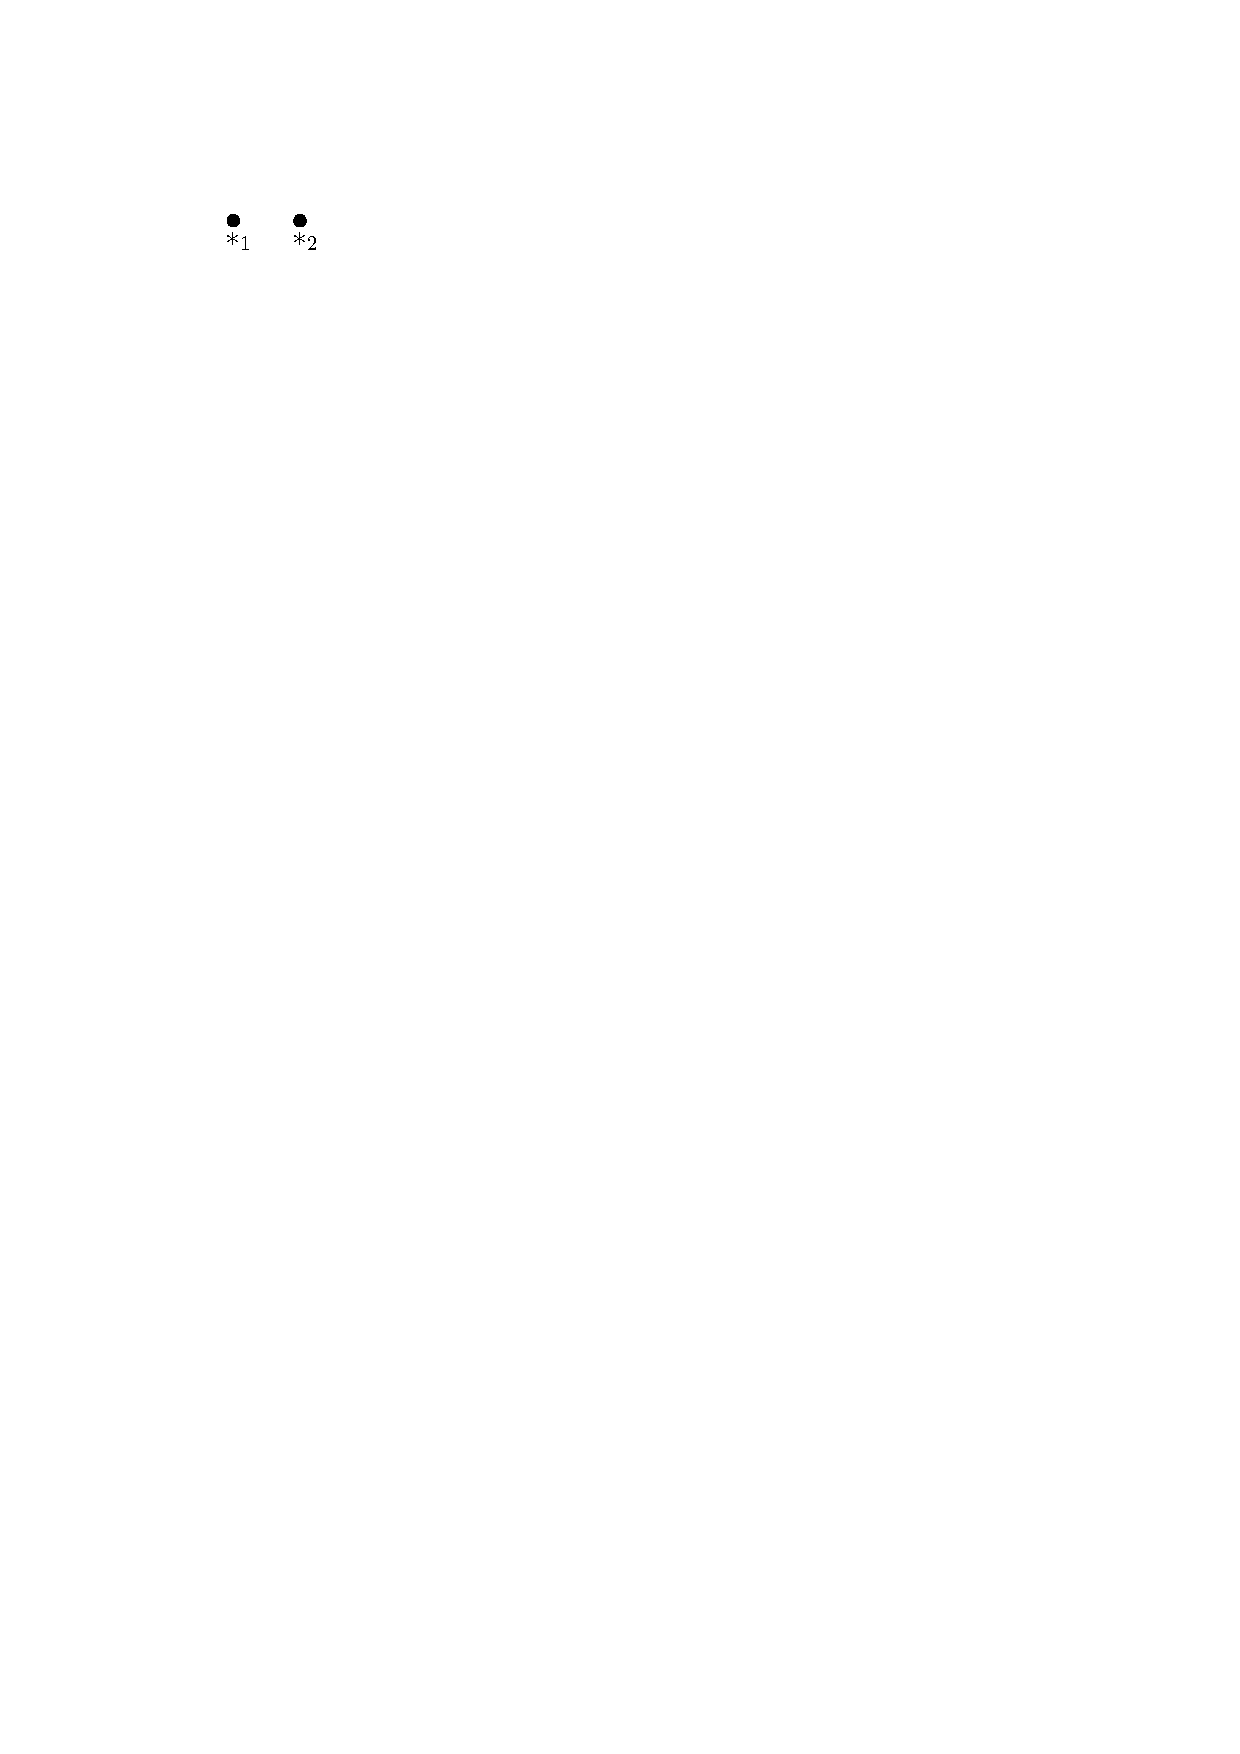
\includegraphics[scale=0.5]{fig/pts2}}\circ_{\ast_1} g_1)\circ_{\ast_2} g_2$.
% \end{example}

These definitions given, it is natural to search for a smallest family of generators of
$\K \G$. The search of such a family is computationally hard. With the help of the computer,
we obtain that the generators of $\K \G$ of arity no more than $5$ are
\begin{equation}\begin{split} \label{equ:generators_G}
    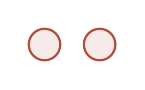
\begin{tikzpicture}[Centering,scale=.7]
        \node[NodeGraph](a)at(0,0){};
        \node[NodeGraph](b)at(1,0){};
    \end{tikzpicture},
    \enspace
    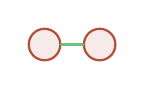
\begin{tikzpicture}[Centering,scale=.7]
        \node[NodeGraph](a)at(0,0){};
        \node[NodeGraph](b)at(1,0){};
        \draw[EdgeGraph](a)--(b);
    \end{tikzpicture},
    \qquad
    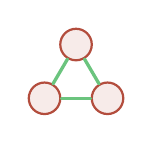
\begin{tikzpicture}[Centering,scale=.4]
        \node[NodeGraph](a)at(-1,-1){};
        \node[NodeGraph](b)at(1,-1){};
        \node[NodeGraph](c)at(0,.707){};
        \draw[EdgeGraph](a)--(b);
        \draw[EdgeGraph](a)--(c);
        \draw[EdgeGraph](b)--(c);
    \end{tikzpicture},
    \qquad
    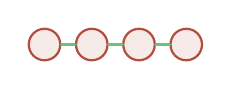
\begin{tikzpicture}[Centering,scale=.6]
        \node[NodeGraph](a)at(0,0){};
        \node[NodeGraph](b)at(1,0){};
        \node[NodeGraph](c)at(2,0){};
        \node[NodeGraph](d)at(3,0){};
        \draw[EdgeGraph](a)--(b);
        \draw[EdgeGraph](b)--(c);
        \draw[EdgeGraph](c)--(d);
    \end{tikzpicture},
    \enspace
    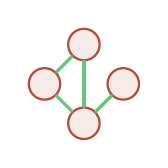
\begin{tikzpicture}[Centering,scale=.5]
        \node[NodeGraph](a)at(-1,-1){};
        \node[NodeGraph](b)at(-1,1){};
        \node[NodeGraph](c)at(0,0){};
        \node[NodeGraph](d)at(-2,0){};
        \draw[EdgeGraph](a)--(b);
        \draw[EdgeGraph](a)--(c);
        \draw[EdgeGraph](a)--(d);
        \draw[EdgeGraph](b)--(d);
    \end{tikzpicture},
    \enspace
    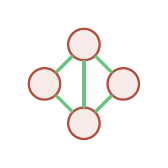
\begin{tikzpicture}[Centering,scale=.5]
        \node[NodeGraph](a)at(-1,-1){};
        \node[NodeGraph](b)at(-1,1){};
        \node[NodeGraph](c)at(0,0){};
        \node[NodeGraph](d)at(-2,0){};
        \draw[EdgeGraph](a)--(b);
        \draw[EdgeGraph](a)--(c);
        \draw[EdgeGraph](a)--(d);
        \draw[EdgeGraph](b)--(c);
        \draw[EdgeGraph](b)--(d);
    \end{tikzpicture},
    \enspace
    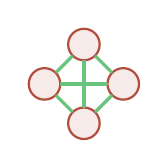
\begin{tikzpicture}[Centering,scale=.5]
        \node[NodeGraph](a)at(-1,-1){};
        \node[NodeGraph](b)at(-1,1){};
        \node[NodeGraph](c)at(0,0){};
        \node[NodeGraph](d)at(-2,0){};
        \draw[EdgeGraph](a)--(b);
        \draw[EdgeGraph](a)--(c);
        \draw[EdgeGraph](a)--(d);
        \draw[EdgeGraph](b)--(c);
        \draw[EdgeGraph](b)--(d);
        \draw[EdgeGraph](c)--(d);
    \end{tikzpicture},
    \\
    \quad
    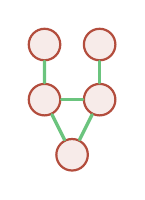
\begin{tikzpicture}[Centering,scale=.35]
        \node[NodeGraph](a)at(-2,0){};
        \node[NodeGraph](b)at(0,0){};
        \node[NodeGraph](c)at(-2,2){};
        \node[NodeGraph](d)at(0,2){};
        \node[NodeGraph](e)at(-1,-2){};
        \draw[EdgeGraph](a)--(b);
        \draw[EdgeGraph](a)--(c);
        \draw[EdgeGraph](a)--(e);
        \draw[EdgeGraph](b)--(d);
        \draw[EdgeGraph](b)--(e);
    \end{tikzpicture},
    \enspace
    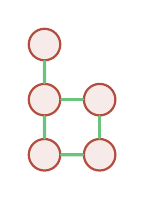
\begin{tikzpicture}[Centering,scale=.35]
        \node[NodeGraph](a)at(-2,0){};
        \node[NodeGraph](b)at(0,-2){};
        \node[NodeGraph](c)at(-2,2){};
        \node[NodeGraph](d)at(0,0){};
        \node[NodeGraph](e)at(-2,-2){};
        \draw[EdgeGraph](a)--(c);
        \draw[EdgeGraph](a)--(d);
        \draw[EdgeGraph](a)--(e);
        \draw[EdgeGraph](b)--(d);
        \draw[EdgeGraph](b)--(e);
    \end{tikzpicture},
    \enspace
    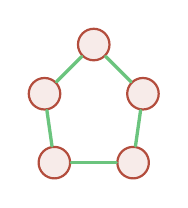
\begin{tikzpicture}[Centering,scale=.5]
        \node[NodeGraph](a)at(-1,-1){};
        \node[NodeGraph](b)at(-1.25,.75){};
        \node[NodeGraph](c)at(0,2){};
        \node[NodeGraph](d)at(1.25,.75){};
        \node[NodeGraph](e)at(1,-1){};
        \draw[EdgeGraph](a)--(b);
        \draw[EdgeGraph](b)--(c);
        \draw[EdgeGraph](c)--(d);
        \draw[EdgeGraph](d)--(e);
        \draw[EdgeGraph](e)--(a);
    \end{tikzpicture},
    \enspace
    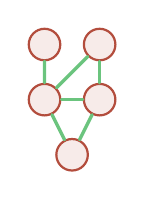
\begin{tikzpicture}[Centering,scale=.35]
        \node[NodeGraph](a)at(-2,0){};
        \node[NodeGraph](b)at(0,0){};
        \node[NodeGraph](c)at(-2,2){};
        \node[NodeGraph](d)at(0,2){};
        \node[NodeGraph](e)at(-1,-2){};
        \draw[EdgeGraph](a)--(b);
        \draw[EdgeGraph](a)--(c);
        \draw[EdgeGraph](a)--(d);
        \draw[EdgeGraph](a)--(e);
        \draw[EdgeGraph](b)--(d);
        \draw[EdgeGraph](b)--(e);
    \end{tikzpicture},
    \enspace
    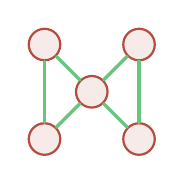
\begin{tikzpicture}[Centering,scale=.6]
        \node[NodeGraph](a)at(0,0){};
        \node[NodeGraph](b)at(1,-1){};
        \node[NodeGraph](c)at(-1,1){};
        \node[NodeGraph](d)at(1,1){};
        \node[NodeGraph](e)at(-1,-1){};
        \draw[EdgeGraph](a)--(b);
        \draw[EdgeGraph](a)--(c);
        \draw[EdgeGraph](a)--(d);
        \draw[EdgeGraph](a)--(e);
        \draw[EdgeGraph](b)--(d);
        \draw[EdgeGraph](c)--(e);
    \end{tikzpicture},
    \enspace
    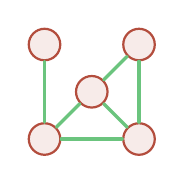
\begin{tikzpicture}[Centering,scale=.6]
        \node[NodeGraph](a)at(0,0){};
        \node[NodeGraph](b)at(1,-1){};
        \node[NodeGraph](c)at(-1,1){};
        \node[NodeGraph](d)at(1,1){};
        \node[NodeGraph](e)at(-1,-1){};
        \draw[EdgeGraph](a)--(b);
        \draw[EdgeGraph](a)--(d);
        \draw[EdgeGraph](a)--(e);
        \draw[EdgeGraph](b)--(d);
        \draw[EdgeGraph](b)--(e);
        \draw[EdgeGraph](c)--(e);
    \end{tikzpicture},
    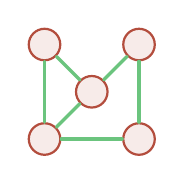
\begin{tikzpicture}[Centering,scale=.6]
        \node[NodeGraph](a)at(0,0){};
        \node[NodeGraph](b)at(1,-1){};
        \node[NodeGraph](c)at(-1,1){};
        \node[NodeGraph](d)at(1,1){};
        \node[NodeGraph](e)at(-1,-1){};
        \draw[EdgeGraph](a)--(c);
        \draw[EdgeGraph](a)--(d);
        \draw[EdgeGraph](a)--(e);
        \draw[EdgeGraph](b)--(d);
        \draw[EdgeGraph](b)--(e);
        \draw[EdgeGraph](c)--(e);
    \end{tikzpicture},
    \\
    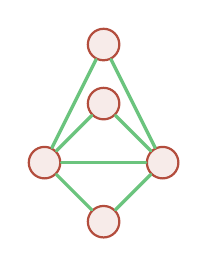
\begin{tikzpicture}[Centering,scale=.5]
        \node[NodeGraph](a)at(0,-1){};
        \node[NodeGraph](b)at(3,-1){};
        \node[NodeGraph](c)at(1.5,2){};
        \node[NodeGraph](d)at(1.5,.5){};
        \node[NodeGraph](e)at(1.5,-2.5){};
        \draw[EdgeGraph](a)--(b);
        \draw[EdgeGraph](a)--(c);
        \draw[EdgeGraph](a)--(d);
        \draw[EdgeGraph](a)--(e);
        \draw[EdgeGraph](b)--(c);
        \draw[EdgeGraph](b)--(d);
        \draw[EdgeGraph](b)--(e);
    \end{tikzpicture},
    \enspace
    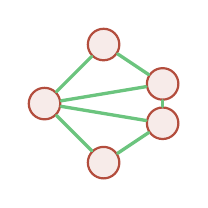
\begin{tikzpicture}[Centering,scale=.5]
        \node[NodeGraph](a)at(0,-1.5){};
        \node[NodeGraph](b)at(3,-1){};
        \node[NodeGraph](c)at(3,-2){};
        \node[NodeGraph](d)at(1.5,0){};
        \node[NodeGraph](e)at(1.5,-3){};
        \draw[EdgeGraph](a)--(b);
        \draw[EdgeGraph](a)--(c);
        \draw[EdgeGraph](a)--(d);
        \draw[EdgeGraph](a)--(e);
        \draw[EdgeGraph](b)--(c);
        \draw[EdgeGraph](b)--(d);
        \draw[EdgeGraph](c)--(e);
    \end{tikzpicture},
    \enspace
    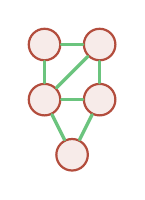
\begin{tikzpicture}[Centering,scale=.7]
        \node[NodeGraph](a)at(0,0){};
        \node[NodeGraph](b)at(1,1){};
        \node[NodeGraph](c)at(.5,-1){};
        \node[NodeGraph](d)at(0,1){};
        \node[NodeGraph](e)at(1,0){};
        \draw[EdgeGraph](a)--(b);
        \draw[EdgeGraph](a)--(c);
        \draw[EdgeGraph](a)--(d);
        \draw[EdgeGraph](a)--(e);
        \draw[EdgeGraph](b)--(d);
        \draw[EdgeGraph](b)--(e);
        \draw[EdgeGraph](c)--(e);
    \end{tikzpicture},
    \enspace
    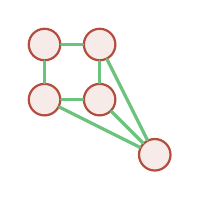
\begin{tikzpicture}[Centering,scale=.7]
        \node[NodeGraph](a)at(0,0){};
        \node[NodeGraph](b)at(1,1){};
        \node[NodeGraph](c)at(2,-1){};
        \node[NodeGraph](d)at(0,1){};
        \node[NodeGraph](e)at(1,0){};
        \draw[EdgeGraph](a)--(c);
        \draw[EdgeGraph](a)--(d);
        \draw[EdgeGraph](a)--(e);
        \draw[EdgeGraph](b)--(c);
        \draw[EdgeGraph](b)--(d);
        \draw[EdgeGraph](b)--(e);
        \draw[EdgeGraph](c)--(e);
    \end{tikzpicture},
    \enspace
    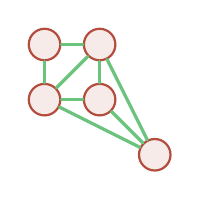
\begin{tikzpicture}[Centering,scale=.7]
        \node[NodeGraph](a)at(0,0){};
        \node[NodeGraph](b)at(1,1){};
        \node[NodeGraph](c)at(2,-1){};
        \node[NodeGraph](d)at(0,1){};
        \node[NodeGraph](e)at(1,0){};
        \draw[EdgeGraph](a)--(b);
        \draw[EdgeGraph](a)--(c);
        \draw[EdgeGraph](a)--(d);
        \draw[EdgeGraph](a)--(e);
        \draw[EdgeGraph](b)--(c);
        \draw[EdgeGraph](b)--(d);
        \draw[EdgeGraph](b)--(e);
        \draw[EdgeGraph](c)--(e);
    \end{tikzpicture},
    \enspace
    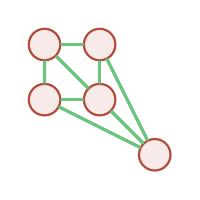
\begin{tikzpicture}[Centering,scale=.7,rotate=90]
        \node[NodeGraph](a)at(0,0){};
        \node[NodeGraph](b)at(1,1){};
        \node[NodeGraph](c)at(-1,-1){};
        \node[NodeGraph](d)at(0,1){};
        \node[NodeGraph](e)at(1,0){};
        \draw[EdgeGraph](a)--(b);
        \draw[EdgeGraph](a)--(c);
        \draw[EdgeGraph](a)--(d);
        \draw[EdgeGraph](a)--(e);
        \draw[EdgeGraph](b)--(d);
        \draw[EdgeGraph](b)--(e);
        \draw[EdgeGraph](c)--(d);
        \draw[EdgeGraph](c)--(e);
    \end{tikzpicture},
    \enspace
    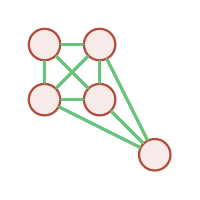
\begin{tikzpicture}[Centering,scale=.7,rotate=90]
        \node[NodeGraph](a)at(0,0){};
        \node[NodeGraph](b)at(1,1){};
        \node[NodeGraph](c)at(-1,-1){};
        \node[NodeGraph](d)at(0,1){};
        \node[NodeGraph](e)at(1,0){};
        \draw[EdgeGraph](a)--(b);
        \draw[EdgeGraph](a)--(c);
        \draw[EdgeGraph](a)--(d);
        \draw[EdgeGraph](a)--(e);
        \draw[EdgeGraph](b)--(d);
        \draw[EdgeGraph](b)--(e);
        \draw[EdgeGraph](c)--(d);
        \draw[EdgeGraph](c)--(e);
        \draw[EdgeGraph](d)--(e);
    \end{tikzpicture},
    \enspace
    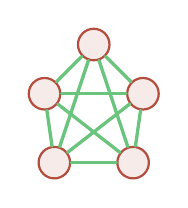
\begin{tikzpicture}[Centering,scale=.5]
        \node[NodeGraph](a)at(-1,-1){};
        \node[NodeGraph](b)at(-1.25,.75){};
        \node[NodeGraph](c)at(0,2){};
        \node[NodeGraph](d)at(1.25,.75){};
        \node[NodeGraph](e)at(1,-1){};
        \draw[EdgeGraph](a)--(b);
        \draw[EdgeGraph](a)--(c);
        \draw[EdgeGraph](a)--(d);
        \draw[EdgeGraph](a)--(e);
        \draw[EdgeGraph](b)--(c);
        \draw[EdgeGraph](b)--(d);
        \draw[EdgeGraph](b)--(e);
        \draw[EdgeGraph](c)--(d);
        \draw[EdgeGraph](c)--(e);
        \draw[EdgeGraph](d)--(e);
    \end{tikzpicture}.
\end{split}\end{equation}
Due to the symmetric group action on $\K \G$, only the knowledge of the shapes of the graphs
is significant. While~\eqref{equ:generators_G} does not provide to us any particular
insight on a possible characterisation of the generators, it does suggest that any graph
with enough edges must be a generator. This is confirmed by the following lemma.

\begin{lemma} \label{lem:infinite_number_generators_G}
Let $\{V_i\}_{i\in I}$ be a family of non empty finite sets, $\{g_i\}_{i \in I}$ be a family
of graphs such that $g_i \in\G[V_i]$, and let $g$ be a graph in $\G[V]$ with at least
$\binom{n-1}{2} +1$ edges, where $n = |V|$. Then $g$ is generated by $\{g_i\}_{i\in I}$ if
and only if $g=g_i$ for some $i\in I$.
\end{lemma}

\begin{proof}
Suppose that $g\not\in\{g_i\}_{i\in I}$. It is sufficient to show that $g$ can not appear 
in the support of any vector of the form $g_1\circ_{\ast} g_2$ for any $g_1$ and $g_2$ 
different from $g$. Hence let $V_1$ and $V_2$ be two disjoint finite sets such that 
$V_1\sqcup V_2 = V$, $g_1\in G'[V_1]$ and $g_2\in G[V_2]$, and denote by $e_1$ the number 
of edges of $g_1$ and by $e_2$ the number of edges of $g_2$. Then the graphs in the support 
of $g_1\circ_{\ast} g_2$ have $e_1+e_2$ edges. This is maximal when $g_1$ and $g_2$ are 
both complete graphs and is then equal to $\binom{x}{2}+\binom{n-x}{2} = x^2-nx+\binom{n}{2}$ 
where $0\leq x=|V_1|\leq n-1$.

If $x = 0$ then necessarily $g_1 =\emptyset_{\ast}$ and $g\in \text{Supp}(g_1\circ_{\ast}g_2) 
= \text{Supp}(g_2)$ if and only if $g=g_2$. This is impossible, hence $x\not = 0$. The expression 
$x^2-nx+\binom{n}{2}$ is then maximal for $x=1$ or $x=n-1$ and is equal in both cases to 
$\binom{n-1}{2}<\binom{n-1}{2} +1$. This implies that $g$ can not be in the support of $g_1\circ_{\ast} g_2$.
\end{proof}

\begin{proposition} \label{gc}
    The operad $\K \G$ is not free and has an infinite number of generators.
\end{proposition}
\begin{proof}
The fact that $\K \G$ has an infinite number of generators is a direct consequence of
Lemma~\ref{lem:infinite_number_generators_G}. Moreover, the relation
\begin{equation}\begin{split} \label{nf}
    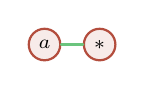
\begin{tikzpicture}[Centering,scale=.7]
        \node[NodeGraph](a)at(0,0){$a$};
        \node[NodeGraph](s)at(1,0){$\ast$};
        \draw[EdgeGraph](a)--(s);
    \end{tikzpicture}
    &
    \circ_\ast
    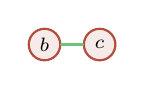
\begin{tikzpicture}[Centering,scale=.7]
        \node[NodeGraph](b)at(0,0){$b$};
        \node[NodeGraph](c)at(1,0){$c$};
        \draw[EdgeGraph](b)--(c);
    \end{tikzpicture}
    \enspace + \enspace
    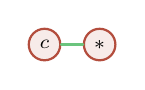
\begin{tikzpicture}[Centering,scale=.7]
        \node[NodeGraph](c)at(0,0){$c$};
        \node[NodeGraph](s)at(1,0){$\ast$};
        \draw[EdgeGraph](c)--(s);
    \end{tikzpicture}
    \circ_\ast
    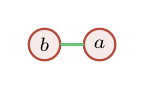
\begin{tikzpicture}[Centering,scale=.7]
        \node[NodeGraph](b)at(0,0){$b$};
        \node[NodeGraph](a)at(1,0){$a$};
        \draw[EdgeGraph](b)--(a);
    \end{tikzpicture}
    \enspace - \enspace
    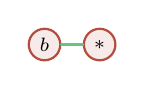
\begin{tikzpicture}[Centering,scale=.7]
        \node[NodeGraph](b)at(0,0){$b$};
        \node[NodeGraph](s)at(1,0){$\ast$};
        \draw[EdgeGraph](b)--(s);
    \end{tikzpicture}
    \circ_\ast
    \begin{tikzpicture}[Centering,scale=.7]
        \node[NodeGraph](a)at(0,0){$a$};
        \node[NodeGraph](c)at(1,0){$c$};
        \draw[EdgeGraph](a)--(c);
    \end{tikzpicture}
    \enspace
    - 2 \,
    \begin{tikzpicture}[Centering,scale=.7]
        \node[NodeGraph](a)at(0,0){$a$};
        \node[NodeGraph](b)at(1,0){$b$};
        \node[NodeGraph](c)at(2,0){$c$};
        \draw[EdgeGraph](a)--(b);
        \draw[EdgeGraph](b)--(c);
    \end{tikzpicture}
    \\[.5em]
    & =
    \begin{tikzpicture}[Centering,scale=.7]
        \node[NodeGraph](a)at(0,0){$a$};
        \node[NodeGraph](b)at(1,0){$b$};
        \node[NodeGraph](c)at(2,0){$c$};
        \draw[EdgeGraph](a)--(b);
        \draw[EdgeGraph](b)--(c);
    \end{tikzpicture}
    \enspace + \enspace
    \begin{tikzpicture}[Centering,scale=.7]
        \node[NodeGraph](b)at(0,0){$b$};
        \node[NodeGraph](c)at(1,0){$c$};
        \node[NodeGraph](a)at(2,0){$a$};
        \draw[EdgeGraph](b)--(c);
        \draw[EdgeGraph](c)--(a);
    \end{tikzpicture}
    \enspace + \enspace
    \begin{tikzpicture}[Centering,scale=.7]
        \node[NodeGraph](c)at(0,0){$c$};
        \node[NodeGraph](b)at(1,0){$b$};
        \node[NodeGraph](a)at(2,0){$a$};
        \draw[EdgeGraph](c)--(b);
        \draw[EdgeGraph](b)--(a);
    \end{tikzpicture}
    \enspace + \enspace
    \begin{tikzpicture}[Centering,scale=.7]
        \node[NodeGraph](b)at(0,0){$b$};
        \node[NodeGraph](a)at(1,0){$a$};
        \node[NodeGraph](c)at(2,0){$c$};
        \draw[EdgeGraph](b)--(a);
        \draw[EdgeGraph](a)--(c);
    \end{tikzpicture}
    \\[.5em]
    & \qquad - \enspace
    \begin{tikzpicture}[Centering,scale=.7]
        \node[NodeGraph](b)at(0,0){$b$};
        \node[NodeGraph](a)at(1,0){$a$};
        \node[NodeGraph](c)at(2,0){$c$};
        \draw[EdgeGraph](b)--(a);
        \draw[EdgeGraph](a)--(c);
    \end{tikzpicture}
    \enspace - \enspace
    \begin{tikzpicture}[Centering,scale=.7]
        \node[NodeGraph](a)at(0,0){$a$};
        \node[NodeGraph](c)at(1,0){$c$};
        \node[NodeGraph](b)at(2,0){$b$};
        \draw[EdgeGraph](a)--(c);
        \draw[EdgeGraph](c)--(b);
    \end{tikzpicture}
    - 2 \,
    \begin{tikzpicture}[Centering,scale=.7]
        \node[NodeGraph](a)at(0,0){$a$};
        \node[NodeGraph](b)at(1,0){$b$};
        \node[NodeGraph](c)at(2,0){$c$};
        \draw[EdgeGraph](a)--(b);
        \draw[EdgeGraph](b)--(c);
    \end{tikzpicture}
    \\[.5em]
    & = 0
\end{split}\end{equation}
shows that $\K \G$ is not free.
\end{proof}

As a consequence of Proposition~\ref{gc}, it seems particularly hard to further
investigate the structure of $\K \G$. Let us restrict further to its suboperad $\K \T$ of
trees. The generators of $\K \T$ until arity $6$ are
\begin{equation}\begin{split}
    \begin{tikzpicture}[Centering,scale=.7]
        \node[NodeGraph](a)at(0,0){};
        \node[NodeGraph](b)at(1,0){};
        \draw[EdgeGraph](a)--(b);
    \end{tikzpicture},
    \qquad
    \begin{tikzpicture}[Centering,scale=.6]
        \node[NodeGraph](a)at(0,0){};
        \node[NodeGraph](b)at(1,0){};
        \node[NodeGraph](c)at(2,0){};
        \node[NodeGraph](d)at(3,0){};
        \draw[EdgeGraph](a)--(b);
        \draw[EdgeGraph](b)--(c);
        \draw[EdgeGraph](c)--(d);
    \end{tikzpicture},
    \qquad
    \begin{tikzpicture}[Centering,scale=.6]
        \node[NodeGraph](a)at(0,0){};
        \node[NodeGraph](b)at(-1,0){};
        \node[NodeGraph](c)at(0,1){};
        \node[NodeGraph](d)at(1,0){};
        \node[NodeGraph](e)at(-2,0){};
        \draw[EdgeGraph](a)--(b);
        \draw[EdgeGraph](a)--(c);
        \draw[EdgeGraph](a)--(d);
        \draw[EdgeGraph](b)--(e);
    \end{tikzpicture},
    \qquad
    \begin{tikzpicture}[Centering,scale=.6]
        \node[NodeGraph](a)at(0,0){};
        \node[NodeGraph](b)at(-1,0){};
        \node[NodeGraph](c)at(0,1){};
        \node[NodeGraph](d)at(1,0){};
        \node[NodeGraph](e)at(0,-1){};
        \node[NodeGraph](f)at(-2,0){};
        \draw[EdgeGraph](a)--(b);
        \draw[EdgeGraph](a)--(c);
        \draw[EdgeGraph](a)--(d);
        \draw[EdgeGraph](a)--(e);
        \draw[EdgeGraph](b)--(f);
    \end{tikzpicture},
    \enspace
    \begin{tikzpicture}[Centering,scale=.6]
        \node[NodeGraph](a)at(0,0){};
        \node[NodeGraph](b)at(-1,0){};
        \node[NodeGraph](c)at(1,-1){};
        \node[NodeGraph](d)at(1,1){};
        \node[NodeGraph](e)at(-2,-1){};
        \node[NodeGraph](f)at(-2,1){};
        \draw[EdgeGraph](a)--(b);
        \draw[EdgeGraph](a)--(c);
        \draw[EdgeGraph](a)--(d);
        \draw[EdgeGraph](b)--(e);
        \draw[EdgeGraph](b)--(f);
    \end{tikzpicture},
    \enspace
    \begin{tikzpicture}[Centering,scale=.6]
        \node[NodeGraph](a)at(0,0){};
        \node[NodeGraph](b)at(1,0){};
        \node[NodeGraph](c)at(2,0){};
        \node[NodeGraph](d)at(3,0){};
        \node[NodeGraph](e)at(4,0){};
        \node[NodeGraph](f)at(2,1){};
        \draw[EdgeGraph](a)--(b);
        \draw[EdgeGraph](b)--(c);
        \draw[EdgeGraph](c)--(d);
        \draw[EdgeGraph](d)--(e);
        \draw[EdgeGraph](c)--(f);
    \end{tikzpicture}.
\end{split}\end{equation}
%In the same way as before, one can show that $\K \T$ has an infinite number of generators.
This operad $\K \T$ has a non trivial link with the pre-Lie operad $\PLie$~\cite{CL01}.
Recall that $\PLie$ can be seen as an operad structure on $\K T^{\bullet}$.
\begin{proposition} \label{prelie}
	The monomorphism of species $\psi : \K \T \to \K \T^{\bullet}$ defined, for any tree
	$t \in \T[V]$ by
	\begin{equation}
	    \psi(t) =  \sum_{r \in V} (t, r),
	\end{equation}
	is a monomorphism of operads from $\K \T$ to $\PLie$.
\end{proposition}

\begin{proof}
Let $t\in T[V]$ be a tree and $r,v\in V$. Denote by $n_t(v)$ the set of neighbours of 
$v$ in $t$ and denote by $c_{t,r}(v)$ the set of children of $v$ when $t$ is rooted 
on $r$, i.e $c_{t,r}(v)= n_{>}(v)$ in $t_r$. If $r\not = v$, further denote by 
$p_{t,r}(v)$ the parent of $v$ in $t$ when $t$ is rooted on $r$ i.e 
$\{p_{t,r}(v)\} = n_{\_}(v)$ in $t_r$.

Let $V_1$ and $V_2$ be two disjoint sets and $t_1\in T'[V_1]$ and $t_2\in T[V_2]$. We have:
\begin{equation}\begin{split}
	\psi_{V_1}(t_1)\circ_{\ast} \psi_{V_2}(t_2) 
	&= \sum_{r_1\in V_1+\{\ast\}} (t_1,r_1) \circ_{\ast} \sum_{r_2\in V_2}(t_2,r_2) \\
	&= \sum_{r_1\in V_1+\{\ast\}}\sum_{r_2\in V_2} (t_1,r_1)\circ_{\ast} (t_2,r_2) \\ 
	&= \sum_{r_1\in V_1}\sum_{r_2\in V_2} \left(t_1\cap V_1^2\oplus p_{t_1,r_1}(\ast)r_2
	\oplus t_2 \oplus \bigoplus_{v\in c_{t_1,r_1}(\ast)} \left(\sum V_2\right)v, r_1\right) \\
	&\quad + \sum_{r_2\in V_2}\left(t_1\cap V_1^2\oplus t_2 \oplus \bigoplus_{v\in c_{t_1,\ast}(\ast)} 
	\left(\sum V_2\right)v,r_2\right) \\
	&= \sum_{r_1\in V_1} \left(t_1\cap V_1^2\oplus p_{t_1,r_1}(\ast)\left(\sum V_2\right) 
	\oplus t_2 \oplus \bigoplus_{v\in c_{t_1,r_1}(\ast)} \left(\sum V_2\right)v, r_1\right) \\
	&\quad+ \sum_{r_2\in V_2} \left(t_1\cap V_1^2\oplus t_2 \oplus \bigoplus_{v\in c_{t_1,\ast}(\ast)} 
	\left(\sum V_2\right)v,r_2\right) \\
	&= \sum_{r\in V_1+V_2}\left(t_1\cap V_1^2\oplus\bigoplus_{v\in n_{t_1}(\ast)}\left(\sum V_2\right)v
	\oplus t_2,r\right) \\
	&= \sum_{r\in V_1+V_2} \left(t_1|_{\ast \leftarrow \sum V_2}\oplus t_2,r\right) \\
	&= \psi_{V_1+V_2}(t_1\circ_{\ast} t_2)
\end{split}\end{equation}
\end{proof}

% Given this morphism we have the following diagram.
% \begin{center}\label{diag}
% \begin{tikzcd}
% 	\PLie \arrow[r, hook, dashed] & ? \\
% 	\K T \arrow[u, hook, "\psi"] \arrow[r, hook] & \K G_c \arrow[u, hook, "\psi ?"]
% \end{tikzcd}
% \end{center}

A natural question to ask is how to extend this morphism to $\K \G_c$ and $\K \MG_c$. Let us
introduce some notations in order to answer this question. For $g\in \MG_c[V]$, $r\in V$,
and $t\in \T[V]$ a spanning tree of $g$, let $\overrightarrow{g}^{(t,r)}\in \MG_{orc}$ be
the oriented multigraph obtained by labelling the edges of $g$ in $t$ in the same way as the
edges of $t_r$, and by labelling both ends of the edges in $g$ not in $t$. More formally, we
have: $\overrightarrow{g}^{(t,r)}=t_{r}\oplus\iota_{\G}(g\setminus t)$, where $\iota: \K
\MG\rightarrow \K \MG_{or}$ sends a multigraph to the oriented multigraph obtained by
labelling all the edges ends.


Define $\K \Operad_2\subset \K\Operad_1\subset\K \ST$ three subspecies of $\K
\MG_{orc}^{\bullet}$ by
\begin{equation}
    \ST[V]=\left\{
        (\overrightarrow{g}^{(t,r)},r) : g\in \MG_c[V], r\in V \text{ and $t$ a
    spanning tree of $g$}\right\},
\end{equation}
\begin{equation}
    \Operad_1[V] = \left\{\sum_{r\in V} (\overrightarrow{g}^{(t(r),r)},r) : g\in
    \MG_c[V]\text{ and for each $r$, $t(r)$ a spanning tree of $g$}\right\},
\end{equation}
\begin{multline}
    \Operad_2[V]=
    \left\{(\overrightarrow{g}^{(t_1,r)},r)-(\overrightarrow{g}^{(t_2,r)},r) : g\in
    \MG_c[V],r\in V,
    \right. \\ \left.
    \text{ and $t_1$ and $t_2$ two spanning trees of $g$}\right\}.
\end{multline}


\begin{lemma} \label{lemmfond}
The following properties hold:
\begin{itemize}
	\item $\K \ST$ is a suboperad of $\K \MG_{orc}^{\bullet}$ isomorphic to $\K\MG\times\PLie$,
	\item $\K \Operad_1$ is a suboperad of $\K \ST$, 
	\item $\K\Operad_2$ is an ideal of $\K\Operad_1$.
\end{itemize}
\end{lemma}

\begin{proof}
\begin{itemize}
	\item The species morphism $\K \MG\times \PLie \hookrightarrow \K \MG^{\bullet}_{orc}$ given by 
	$(g,(t,r)) \mapsto (\overrightarrow{g}^{(t,r)}, r)$ is an operad morphism and hence its image $\ST$ 
	is a suboperad of $ \K MG^{\bullet}_{orc}$.
\end{itemize}
In order to prove the two next items we first prove give equalities. Let $U:\K MG_{or} \rightarrow \K MG$ 
be the forgetful functor which sends an oriented graph on the graph obtained by forgetting the 
orientation (i.e the labels). Let $V_1$ and $V_2$ be two disjoint sets, $g_1\in \MG_c'[V_1]$ 
and $g_2\in \MG_c[V_2]$ be two connected multigraphs, $t$ a spanning tree of $g_1$ and 
for each $v\in V_2$, $t(v)$ a spanning tree of $g_2$. Then, for $r\in V_2$
\begin{equation} \begin{split}\label{eq1}
	U\times\id&\left((\overrightarrow{g_1}^{(t,\ast)},\ast)\circ_{\ast}(\overrightarrow{g_2}^{(t(r),r)},r)\right) \\
	&= \left(g_1\cap V_1 \oplus\bigoplus_{v\in n(\ast)}v(\sum V_2)\oplus((\sum V_2)^2)^{\oplus g_1(\ast\ast)}\oplus g_2, r\right) \\
	&= (g_1\circ_{\ast}g_2, r).
\end{split} \end{equation}
Let now $r$ be a vertex in $V_1$. Denote by $p$ the parent of $\ast$ in $t_r$, by $c(\ast)$ 
the children of $\ast$ in $t_r$, by $n_{g_1\setminus t}(\ast)$ the multiset of neighbours
of $\ast$ in $g_1\setminus t$ and by $n(\ast)$ the multiset of neighbours of $\ast$ in 
$g_1$, so that $n(\ast)=n_{g_1\setminus t}(\ast)\cup c(\ast)\cup \{p\}$. Then
\begin{equation} \begin{split}\label{eq2}
	U\times\id&\left((\overrightarrow{g_1}^{(t,r)},r)\circ_{\ast}\sum_{v\in V_2}(\overrightarrow{g_2}^{(t(v),v)},v) \right) \\
	&= \sum_{v\in V_2} U\times\id\left((\overrightarrow{g_1}^{(t,r)},r)\circ_{\ast}\sum_{v\in V_2}(\overrightarrow{g_2}^{(t(v),v)},v) \right) \\
	&= \sum_{v\in V_2}\left(g_1\cap V_1^2\oplus pv \oplus \bigoplus_{v'\in c(\ast)} v'\left(\sum V_2\right)
		\oplus\bigoplus_{v'\in n_{g_1\setminus t}(\ast)}v'\left(\sum V_2\right) \oplus ((\sum V_2)^2)^{\oplus g_1(\ast\ast)}\oplus g_2, r\right)\\
	&=\left(g_1\cap V_1^2\oplus p\left(\sum V_2\right) \oplus \bigoplus_{v'\in c(\ast)} v'\left(\sum V_2\right)
		\oplus\bigoplus_{v'\in n_{g_1\setminus t}(\ast)}v'\left(\sum V_2\right) \oplus ((\sum V_2)^2)^{\oplus g_1(\ast\ast)}\oplus g_2, r\right) \\
	&= \left(g_1\cap V_1^2\oplus \bigoplus_{v\in n(\ast)} v\left(\sum V_2\right)\oplus ((\sum V_2)^2)^{\oplus g_1(\ast\ast)}\oplus g_2, r\right) \\
	&= (g_1\circ_{\ast} g_2, r).
\end{split} \end{equation}
\begin{itemize}
	%The species $\ST$ is then the intersection of this sub-operad with the sub-operad $\K G^{\bullet}_{orc}$ and hence is an operad (since the intersection of two sub-operads is a sub-operad).
	%\item We have a species isomorphism $\phi:\text{\PLie}\times\K MG\stackrel{\sim}\longrightarrow\K \ST$ given by $\phi_V((t,r),g) = (\overrightarrow{t\oplus g}^{(t,r)},r)$ and $\phi_V^{-1}((\overrightarrow{g}^{(t,r)},r)) = ((t,r),g\setminus t)$. Since $\iota_{\text{\PLie}}$ and $\iota_{MG}$ are both morphisms of operads, this is a morphism of operad, hence the result.
	\item Let $V_1$ and $V_2$ be two disjoint sets, $g_1\in \MG'_c[V_1]$ and $g_2\in \MG_c[V_2]$ 
	be two connected multigraphs and for each $v\in V_1+\{\ast\}$, $t(v)$ a spanning tree of $g_1$ 
	and for each $v\in V_2$, $t(v)$ a spanning tree of $g_2$. We have
	\begin{equation}\begin{split}
		\sum_{r_1\in V_1+\{\ast\}} \overrightarrow{g_1}^{(t(r_1),r_1)} &\circ_{\ast} \sum_{r_2\in V_2} \overrightarrow{g_2}^{(t(r_2),r_2)} 
		= \sum_{r_1\in V_1+\{\ast\}}\sum_{r_2\in V_2} \overrightarrow{g_1}^{(t(r_1),r_1)}\circ_{\ast} \overrightarrow{g_2}^{(t(r_2),r_2)} \\
		&= \sum_{r_1\in V_1+\{\ast\}}\sum_{r_2\in V_2} \left(\overrightarrow{g_1}^{(t(r_1),r_1)}|_{\ast_{\_}\leftarrow r_{2\_},\, \ast_{>}\leftarrow(\sum V_2)_{>}}
		\oplus \overrightarrow{g_2}^{(t(r_2),r_2)}, r_1|_{\ast\leftarrow r_2}\right).
	\end{split}\end{equation}
	Then from \ref{eq1} and \ref{eq2} we know that applying $U\times\id$ to the preceeding sum gives us:
	\begin{equation}
		\sum_{r\in V_1+V_2} (g_1\circ_{\ast}g_2,r).
	\end{equation}
	To conclude remark that $\K\op_1[V]$ can be defined as the reciprocal image of 
	$\K\{\sum_{v\in V}(g,v)\,|\,g\in \MG_c[V]\}$ by $U\times\id: \K \ST\rightarrow \K \MG_c^{\bullet}$.
	\item It is easy to see that $\K\op_2$ is a left ideal of $\K \ST$ and hence of $\K\op_1$. 
	Let $V_1$ and $V_2$ be two disjoint finite sets, $g_1\in \MG'_c[V_1]$ and 
	$g_2\in \MG_c[V_2]$, $r\in V_1$, $t$ a spanning tree of $g_1$ and for every $v\in V_2$, $t(v)$ 
	a spanning tree of $g_2$. Then from \ref{eq1} and \ref{eq2} we know that 
	$U\times\id(\overrightarrow{g_1}^{(t,r)}\circ_{\ast}\sum_{v\in V_2} \overrightarrow{g_2}^{(t(v),v))}$ 
	is of the form $(g_1\circ_{\ast} g_2, r)$ if $r\not = \ast$, and of the form 
	$\sum_{v\in V_2} (g_1\circ_{\ast} g_2, v)$ otherwise. In both cases it does not depend on $t$.
	 This concludes this proof since $\K \op_2[V]$ is the kernel of $(U\times\id)_V: \K \ST[V]\rightarrow \K G_c^{\bullet}[V]$.
\end{itemize}
\end{proof}

We can see $\PLie$ as a suboperad of $\ST$ by the monomorphism
$(t,r)\mapsto (t_r,r)$. The image of the operad morphism $\psi$ of Proposition~\ref{prelie} is
then $\K\Operad_1\cap \PLie$ and we have that $\K\Operad_2\cap \PLie = \{0\}$ and hence
$\K\Operad_1\cap \PLie/\K\Operad_2\cap \PLie = \K\Operad_1\cap \PLie$.


\begin{proposition}
The operad isomorphism $\psi: \K \T \to \PLie$
extends into an operad isomorphism $\psi: \K \MG_c \to \K\Operad_1/\K\Operad_2$ satisfying,
for any $g \in \MG_c[V]$,
\begin{equation}
    \psi(g) = \sum_{r\in V}\overrightarrow{g}^{(t(r),r)},
\end{equation}
where for each $r\in V$, $t(r)$ is a spanning tree of $g$. Furthermore, this isomorphism
restricts itself to an isomorphism $\K\G_C \to \K\Operad_1\cap\K\G_c/\K\Operad_2\cap\K\G_c$.
\end{proposition}

\begin{proof}
This statement is a direct consequence of Lemma \ref{lemmfond} and its proof.
\end{proof}

The last results are summarized in the following commutative diagram of operad morphisms.
\begin{equation}
\begin{tikzcd}
    \K \T \arrow[r, "\sim"] \arrow[d, hook]
    & \PLie\cap\K\Operad_1/\K\Operad_2 \arrow[r, equal] \arrow[d, hook]
    & \PLie\cap\K\Operad_1 \arrow[d,hook] \arrow[r, hook]
    & \PLie \arrow[d,hook]\\
    \K \G_c \arrow[r, "\sim"] \arrow[d, hook]
    & \K\Operad_1\cap\K\G_c/\K\Operad_2\cap\K\G_c \arrow[d, hook]
    & \K\G_{orc}^{\bullet}\cap\K\Operad_1 \arrow[l, two heads] \arrow[r, hook] \arrow[d, hook]
    & \K\G_{orc}^{\bullet}\cap\K \ST \arrow[d, hook] \\
    \K\MG_c \arrow[r, "\sim"]
    & \K\Operad_1/\Operad_2
    & \K\Operad_1 \arrow[l, two heads] \arrow[r, hook]
    & \K\MG\times\PLie
\end{tikzcd}
\end{equation}


\section{Finitely generated suboperads} \label{sec:suboperads}
Let us now focus on finitely generated suboperads of $\K \G$.  First remark that the 
suboperad of $\K \G$ generated by
\begin{math}
    \left\{
    \begin{tikzpicture}[Centering,scale=.6]
        \node[NodeGraph](a)at(0,0){$a$};
        \node[NodeGraph](b)at(1,0){$b$};
    \end{tikzpicture}
    \right\}
\end{math}
is isomorphic to the associative operad $\K \As$. Indeed,
\begin{equation}
    \begin{tikzpicture}[Centering,scale=.7]
        \node[NodeGraph](a)at(0,0){$a$};
        \node[NodeGraph](s)at(1,0){$\ast$};
    \end{tikzpicture}
    \enspace \circ_\ast \enspace
    \begin{tikzpicture}[Centering,scale=.7]
        \node[NodeGraph](b)at(0,0){$b$};
        \node[NodeGraph](c)at(1,0){$c$};
    \end{tikzpicture}
    \enspace = \enspace
    \begin{tikzpicture}[Centering,scale=.7]
        \node[NodeGraph](a)at(0,0){$a$};
        \node[NodeGraph](b)at(1,0){$b$};
        \node[NodeGraph](c)at(2,0){$c$};
    \end{tikzpicture}
    \enspace = \enspace
    \begin{tikzpicture}[Centering,scale=.7]
        \node[NodeGraph](s)at(0,0){$\ast$};
        \node[NodeGraph](c)at(1,0){$c$};
    \end{tikzpicture}
    \enspace \circ_\ast \enspace
    \begin{tikzpicture}[Centering,scale=.7]
        \node[NodeGraph](a)at(0,0){$a$};
        \node[NodeGraph](b)at(1,0){$b$};
    \end{tikzpicture}
\end{equation}

Recall that the set operad $\ComMag$~\cite{BL11} is the free set operad generated by one binary
and symmetric element. More formally, $\ComMag[V]$ is the set of all nonplanar binary trees
with set of leaves equal to $V$. Let $s$ be the connected set species defined by $|s[V]| = 1$ if
$|V|=2$, $|s[V]|=0$ otherwise. The action of transposition on the sole element of
$s[\{a,b\}]$ is trivial. Then $\ComMag = \FreeOp_{s}$.
\begin{proposition} \label{commag}
    The suboperad of $\K \G$ generated by
    \begin{math}
        \left\{
        \begin{tikzpicture}[Centering,scale=.6]
            \node[NodeGraph](a)at(0,0){$a$};
            \node[NodeGraph](b)at(1,0){$b$};
            \draw[EdgeGraph](a)--(b);
        \end{tikzpicture}
        \right\}
    \end{math}
    is isomorphic to $\K \ComMag$.
\end{proposition}

\begin{proof}
We know from Proposition~\ref{prelie} that the operad of the statement
is isomorphic to the
suboperad of $\PLie$ generated by 
\begin{equation}
    \left\{
    \begin{tikzpicture}[Centering,scale=.6]
        \node[RootGraph](a)at(0,0){$a$};
        \node[NodeGraph](b)at(0,-1){$b$};
        \draw[EdgeGraph](a)--(b);
    \end{tikzpicture}
    +
    \begin{tikzpicture}[Centering,scale=.6]
        \node[RootGraph](a)at(0,0){$b$};
        \node[NodeGraph](b)at(0,-1){$a$};
        \draw[EdgeGraph](a)--(b);
    \end{tikzpicture}
    \right\}
\end{equation}
Then~\cite{BL11} gives us that this suboperad is isomorphic to $\K \ComMag$. This concludes
the proof
\end{proof}


The fact that we can see both $\K \As$ and $\K \ComMag$ as suboperads of $\K \G$ gives us
natural way to define the smallest operad containing these two as suboperads. Denote by $G$
the subspecies of $\K\G$ generated by
\begin{math}
    \left\{
    \begin{tikzpicture}[Centering,scale=.6]
        \node[NodeGraph](a)at(0,0){$a$};
        \node[NodeGraph](b)at(1,0){$b$};
    \end{tikzpicture},
    \begin{tikzpicture}[Centering,scale=.6]
        \node[NodeGraph](a)at(0,0){$a$};
        \node[NodeGraph](b)at(1,0){$b$};
        \draw[EdgeGraph](a)--(b);
    \end{tikzpicture}
    \right\}
\end{math}
and $\SP$ the suboperad generated by $G$. This operad has some nice properties.

Given $n$ an integer and a set of rewritting rules $\{v_i\rightarrow w_i\}_{1\leq i\leq n}$ 
the {\em rewriting system generated by these rules} is the rewriting system $(R,S,\phi)$ 
where $R$ is the species generated by the family $\{v_i\}_{1\leq i \leq n}$, $S$ is the 
species generated by $\{w_i\}_{1\leq i \leq n}$ and $\phi$ is the morphism defined by
$\phi(v_i) = w_i$.

\begin{proposition}
    The operad $\SP$ is isomorphic to the operad $\Operad_r$ with $r$ the rewriting
    system over $G$ generated by
     \begin{subequations}
    \begin{equation} \label{equ:rel_1}
        \Points{\ast}{c} \circ^{\xi}_\ast \Points{a}{b}
        \enspace \rightarrow \enspace
        \Points{a}{\ast} \circ^{\xi}_\ast \Points{b}{c},
    \end{equation}
    \begin{center}
    	and
    \end{center}
    \begin{equation} \label{equ:rel_2}
        \Segment{a}{\ast} \circ^{\xi}_\ast \Points{b}{c}
        \enspace \rightarrow \enspace
        \Points{b}{\ast} \circ^{\xi}_\ast \Segment{a}{c}
        \enspace + \enspace
        \Points{c}{\ast} \circ^{\xi}_\ast \Segment{a}{b}.
    \end{equation}
    \end{subequations}
    Furthermore, this rewriting system is convergent. Therefore, $\SP$ is Koszul and
    quadratic.
\end{proposition}

\begin{proof}
Let us first show that this rewriting system is convergent
\end{proof}



\begin{proposition}
    The operad $\SP$ admits as Koszul dual the operad $\SP^!$ which is isomorphic to the
    operad $\Ope(G^{\vee}, R)$ where 
    %$G$ is the subspecies of $\K\G$ generated by $\{\Points{a}{b}, \Segment{a}{b}\}$
    $R$ is the subspecies of $\FreeOp_{G^\vee}$ generated by
    \begin{subequations}
    \begin{equation} \label{equ:rel_dual_1}
        \Segment{a}{\ast}^{\vee} \circ_\ast \Segment{b}{c}^{\vee},
    \end{equation}
    \begin{equation} \label{equ:rel_dual_2}
        \Points{a}{\ast}^{\vee} \circ^{\xi}_\ast \Segment{b}{c}^{\vee}
        \enspace - \enspace
        \Segment{b}{\ast}^{\vee} \circ^{\xi}_\ast \Points{a}{c}^{\vee}
        \enspace - \enspace
        \Points{a}{\ast}^{\vee} \circ^{\xi}_\ast \Segment{b}{c}^{\vee},
    \end{equation}
    \begin{equation} \label{equ:rel_dual_3}
        \Points{a}{\ast}^{\vee} \circ^{\xi}_\ast \Points{b}{c}^{\vee}
        +
        \Points{c}{\ast}^{\vee} \circ^{\xi}_\ast \Points{a}{b}^{\vee}
        +
        \Points{b}{\ast}^{\vee} \circ^{\xi}_\ast \Points{a}{c}^{\vee}.
    \end{equation}
    \end{subequations}
\end{proposition}

\begin{proof}
Let us respectively denote by $r_1$ and $r_2$ the vectors induced by the rewriting rules
elements~\eqref{equ:rel_1} and \eqref{equ:rel_2} and $r'_1$, $r'_2$, and $r'_3$ the vectors 
\eqref{equ:rel_dual_1}, \eqref{equ:rel_dual_2}, and~\eqref{equ:rel_dual_3}. Denote by $I$ 
the operad ideal generated by~$r_1$ and~$r_2$. Then as a vector space, $I[[\{a,b,c\}]]$ 
is the linear span of the set
\begin{equation}
    \{r_1, r_1 \cdot (ab), r_2,r_2 \cdot (abc), r_2 \cdot (acb)\},
\end{equation}
where $\cdot$ is the action of the symmetric group, e.g $r_1\cdot (ab) = \FreeOp_{G}[(ab)](r_1)$. 
This space is a sub-space of dimension $5$ of $\FreeOp_G[\{a,b,c\}]$, which is
of dimension $12$. Hence, since as a vector space
\begin{equation}
	\FreeOp_{G^\vee}[\{a,b,c\}]
	\cong \FreeOp_{G^*}[\{a,b,c\}]\cong
	\FreeOp_{G}[\{a,b,c\}],
\end{equation}
$I^{\bot}[\{a,b,c\}]$ must be of dimension 7.

Denote by $J$ the ideal generated by $r_1'$, $r_2'$ and $r_3'$. Then as a vector space
$J[\{a,b,c\}]$ is the linear span of the set
\begin{equation}
    \{ r_1', r_1'\cdot (ab), r_1'\cdot (ac),r_2', r_2'\cdot (abc),r_2'\cdot (acb), r_3'\}.
\end{equation}
This space is of dimension 7. To conclude we need to show that for
any $f\in J[\{a,b,c\}]$ and $x\in I[\{a,b,c\}]$ we have $<f,x>=0$.
Denote by $p_{a,b} = \Points{a}{b}$ and $s_{a,b} = \Segment{a}{b}$.
\begin{equation}\begin{split}
	<r_1',r_1> &=
	<s_{a,\ast}^{\vee}\circ_{\ast} s_{b,c}^{\vee}\,,\, p_{\ast,c}\circ_{\ast}p_{a,b} -
	p_{a,\ast}\circ_{\ast} p_{b,c}> \\
	&= <s_{a,\ast}^{\vee}\circ_{\ast} s_{b,c}^{\vee}\,,\, p_{\ast,c}\circ_{\ast}p_{a,b}> - <s_{a,\ast}^{\vee}\circ_{\ast} s_{b,c}^{\vee}\,,\,p_{a,\ast}\circ_{\ast} p_{b,c}> \\
	&= s_{a,\ast}^{\vee}(p_{\ast,c})s_{b,c}^{\vee}(p_{a,b}) -
	s_{a,\ast}^{\vee}(p_{a,\ast})s_{b,c}^{\vee}(p_{b,c}) = 0.
\end{split}\end{equation}
\begin{equation}\begin{split}
	<r_1',r_1\cdot (ab)> &=
	<s_{a,\ast}^{\vee}\circ_{\ast} s_{b,c}^{\vee}\,,\, p_{\ast,c}\circ_{\ast}p_{a,b} -
	p_{b,\ast}\circ_{\ast} p_{a,c}> \\
	&= s_{a,\ast}^{\vee}(p_{\ast,c})s_{b,c}^{\vee}(p_{a,b}) -
	s_{a,\ast}^{\vee}(p_{b,\ast})s_{b,c}^{\vee}(p_{a,c}) = 0.
\end{split}\end{equation}
% \begin{equation}\begin{split}
% 	<r_1',r_2> &=
% 	<s_{a,\ast}^{\vee}\circ_{\ast} s_{b,c}^{\vee}\,,\, s_{a,\ast}\circ_{\ast}p_{b,c} -
% 	p_{b,\ast}\circ_{\ast} s_{a,c} - p_{c,\ast}\circ_{\ast} s_{a,b}>  \\
% 	&= s_{a,\ast}^{\vee}(p_{\ast,c})s_{b,c}^{\vee}(p_{a,b}) -
% 	s_{a,\ast}^{\vee}(p_{b,\ast})s_{b,c}^{\vee}(p_{a,c}) = 0.
% \end{split}\end{equation}


\end{proof}


\begin{proposition}
    The Hilbert series of $\SP^{!}$ is 
    \begin{equation}
        \mathcal{H}_{\SP^!}(x) = \dfrac{(1-\log(1-x))^2-1}{2}.
    \end{equation}
\end{proposition}

\begin{proof}
The Hilbert series of $\K\ComMag$ is $\mathcal{H}_{\K\ComMag}(x) = 1-\sqrt{1-2x}$ 
hence the Hilbert series of $\SP\cong E(\K\ComMag)$ is $\mathcal{H}_{\SP}(x)=e^{1-\sqrt{1-2x}}-1$, 
where the $-1$ comes from the fact that we consider positive species. 
We deduce the Hilbert series of $\SP^!$ from $\mathcal{H}_{\SP}$ and the identity \ref{hdual}.
\end{proof}
The first dimensions $\dim \SP^![[n]]$ for $n\geq 1$ are
\begin{equation}
    1, 2, 5, 17, 74, 394, 2484, 18108, 149904.
\end{equation}
This is sequence~\OEIS{A000774} of~\cite{Slo}. This sequence is in particular linked to some
pattern avoiding signed permutations and mesh patterns.

Before ending this section let us mention the suboperad $\LP$ of $\K \MG$ generated by
\begin{equation}
    \left\{
    \begin{tikzpicture}[Centering,scale=.6]
        \tikzset{every loop/.style={}}
        \node[NodeGraph](a)at(0,0){$a$};
        \draw[EdgeGraph](a)edge[loop](a);
    \end{tikzpicture},
    \begin{tikzpicture}[Centering,scale=.6]
        \node[NodeGraph](a)at(0,0){$a$};
        \node[NodeGraph](b)at(1,0){$b$};
    \end{tikzpicture}
    \right\}.
\end{equation}
This operad presents a clear interest since its two generators can be considered as minimal
elements in the sense that a partial composition with the two isolated vertices adds exactly
one vertex and no edges, while a partial composition with the loop adds exactly one edge and
no vertex.  A natural question to ask at this point concerns the description of the
multigraphs generated by these two minimal elements.

\begin{proposition}
The following properties hold:
\begin{itemize}
\item the operad $\SP$ is a suboperad of $\LP$;
\item the operad $\LP$ is a strict suboperad of $\K \MG$. In particular, the multigraph
\begin{equation}
    \begin{tikzpicture}[Centering,scale=.8]
        \node[NodeGraph](a)at(0,0){$a$};
        \node[NodeGraph](b)at(1,0){$b$};
        \node[NodeGraph](c)at(2,0){$c$};
        \draw[EdgeGraph](a)--(b);
        \draw[EdgeGraph](b)edge[bend left=40](c);
        \draw[EdgeGraph](b)edge[bend right=40](c);
    \end{tikzpicture}
\end{equation}
is in $\K \MG$ but is not in $\LP$.
\end{itemize}
\end{proposition}

\begin{proof}
\begin{itemize}
	\item The following show that 
	\begin{math}
    \begin{tikzpicture}[Centering,scale=.6]
        \node[NodeGraph](a)at(0,0){$a$};
        \node[NodeGraph](b)at(1,0){$b$};
        \draw[EdgeGraph](a)--(b);
    \end{tikzpicture}
	\end{math}
	is in $\LP[\{a,b\}]$ and hence that $\SP$ is a suboperad of $\LP$.
	\begin{equation}
        \begin{tikzpicture}[Centering,scale=.6]
        	\tikzset{every loop/.style={}}
        	\node[NodeGraph](a)at(0,0){$\ast$};
        	\draw[EdgeGraph](a)edge[loop](a);
    	\end{tikzpicture}
    	\circ_{\ast}
    	\Points{a}{b}
    	 - 
    	\begin{tikzpicture}[Centering,scale=.6]
        	\tikzset{every loop/.style={}}
        	\node[NodeGraph](a)at(0,0){$a$};
        	\draw[EdgeGraph](a)edge[loop](a);
    	\end{tikzpicture}
    	 - 
		\begin{tikzpicture}[Centering,scale=.6]
        	\tikzset{every loop/.style={}}
        	\node[NodeGraph](a)at(0,0){$b$};
        	\draw[EdgeGraph](a)edge[loop](a);
    	\end{tikzpicture}
    	\enspace = \enspace
    	2 \Segment{a}{b}.
    \end{equation}
    \item This was obtained by exhaustive search using a computer.
\end{itemize}
\end{proof}

\bigskip
\noindent{\bf Concluding remarks}
There are two main questions, with reciprocical goals, raised by this paper: the description
of the multigraphs generated contained in $\LP$ and the description of the generators of the
various operads defined here (as $\K\G_{orc}^{\bullet}$, $\K\G_c$, $\K\T$, {\em etc.}).
Another perspective for future work is to study appropriate examples of algebras on $\SP$
and~$\SP^!$.

\bibliographystyle{plain}
\bibliography{redac}

\end{document}







